\documentclass[11pt]{article}

\usepackage{amsmath,amssymb}
\usepackage[margin=1.0in]{geometry}
\usepackage{bm}
\usepackage{booktabs}
\usepackage{array}
\usepackage{graphicx}
\usepackage{float}
\usepackage{enumitem}
\newcolumntype{P}[1]{>{\raggedright\arraybackslash}p{#1}}
\usepackage[colorlinks=true,linkcolor=blue,citecolor=blue,urlcolor=blue]{hyperref}

\input{marcos.inc}

\numberwithin{equation}{section}
\sloppy
\setlength{\emergencystretch}{3em}
\graphicspath{{figures/benchmarks/}}

% --- notation (follows quasi_static_models.tex) -----------------------------
\newcommand{\R}{\mathbb{R}}
\newcommand{\eps}{\varepsilon}
\newcommand{\dS}{\,\mathrm{d}S}
\newcommand{\dV}{\,\mathrm{d}V}
\newcommand{\vu}{\mathbf{u}}
\newcommand{\vx}{\mathbf{x}}
\newcommand{\vy}{\mathbf{y}}
\newcommand{\vb}{\mathbf{b}}
\newcommand{\vm}{\mathbf{m}}
\newcommand{\vn}{\hat{\mathbf{n}}}
\newcommand{\rhat}{\hat{\mathbf{r}}}
\newcommand{\code}[1]{\texttt{#1}}
\newcommand{\Ylm}{Y_{lm}}
\newcommand{\gradone}{\nabla_{1}}
\newcommand{\review}[1]{\textsuperscript{[\ref{#1}]}}

\title{The benchmarks of \texttt{mfemElasticity}:\\
       what each one tests, against what, and what it shows}
\author{Compiled from \code{benchmarks/}, its drivers and scripts, and the
        stored campaign results}
\date{2 October 2026}

\begin{document}
\maketitle

\begin{abstract}
\noindent
This note goes through the benchmark families of \code{benchmarks/} one at
a time: the Love-number family (load and tidal Love numbers of spherically
layered self-gravitating bodies, across formulations, solvers and
core--mantle-boundary treatments, and the response as fields), the
relabelling family (the mapped/aspherical machinery checked with
the spherical physics unchanged), the perturbation family (derivatives of
the response with respect to an interface radius), and the viscoelastic
family (the time integrators: exact box and sphere benchmarks without
gravity, the time-stepping survey, and Maxwell Love-number histories
against a correspondence-principle reference). For each it states what is tested,
the aim, the assumptions, and the mathematics of the comparison, including
how the reference is obtained. The figures are those of the stored runs,
some redrawn with corrected plotting scripts and a few from small reruns
made for this note (\S\ref{sec:provenance}). \S\ref{sec:figures}
reviews the figures and the talk figures, and
\S\ref{sec:review} lists the points that look like mistakes or
inconsistencies, for later review. Superscripts such as
\textsuperscript{[R3]} in the text point to that list. This note
documents the benchmarks and does not re-derive the methods;
\code{doc/quasi\_static\_models.tex} and the method notes it cites hold
the formulations.
\end{abstract}

\tableofcontents

%=============================================================================
\section{Common setting}
\label{sec:common}
%=============================================================================

\subsection{Organisation}

Each family is a directory of \code{benchmarks/} with its own drivers
(C++, MPI), scripts (Python, run in the directory's poetry environment)
and README. The shared parts are in \code{benchmarks/common/}:

\begin{center}
\begin{tabular}{@{}lP{10.5cm}@{}}
\toprule
file & role \\
\midrule
\code{models.py} & the models, as planetmodel \code{Model}s in SI, and their scaling \\
\code{make\_case.py} & one \emph{case}: mesh, fields on it, manifest, and the pyslfp reference \\
\code{benchmark\_case.hpp} & the drivers' common layer: a case set up as a problem, the harmonic analysis, the centre-of-mass correction, JSON output \\
\code{relabelling.hpp} & the relabellings and interface shifts, exact radial profiles \\
\code{reference\_field.hpp} & the reference solution as fields on the mesh \\
\code{costs.py}, \code{drivers.py} & cost bookkeeping; locating the build's drivers \\
\bottomrule
\end{tabular}
\end{center}

The viscoelastic family has four sub-families of its own,
\code{viscoelastic/box}, \code{viscoelastic/sphere},
\code{viscoelastic/love} and \code{viscoelastic/stepping}
(\S\ref{sec:visco}).

\code{campaign.py} runs every family with one command (profiles
\code{local}, eight ranks, about an hour; \code{server}, 100 ranks, an
$h$-ladder at orders 2 and 3, degrees to 16). All output goes to the build
tree. The \code{local} profile uses the models \code{homogeneous},
\code{two\_solid} and \code{fluid\_core} at $h=0.3$, order 2, degrees
$0$--$4$, DtN degree 16.

\subsection{The physical problem}

All families solve the linearised, quasi-static, self-gravitating
response of a body $M$ with background density $\rho$, bulk and shear
moduli $\kappa,\mu$ and background potential $\Phi_0$, to a surface mass
load $\sigma$ on $\partial M$ or an applied potential $\psi$. The sign
convention throughout the code is $\nabla\Phi_0 = g\,\rhat$ (the potential
increases outward, so the potential of a positive mass is negative). The
unknowns are a displacement $\vu$ and a potential perturbation $\phi$
(Eulerian methods) or $\zeta$ (referential methods), on a computational
ball $B\supset M$ whose outer sphere carries a Dirichlet-to-Neumann (DtN)
condition, truncated at the DtN degree. Between $\partial M$ and $\partial B$
there is a \emph{buffer shell}, $1<r<1.2$, where the potential is solved
too. The formulations (Dahlen's Eulerian form with the fluid eliminated,
the gauged fluid, the welded referential form, the slipping interface)
are set out in \code{doc/quasi\_static\_models.tex}; the benchmarks use
them as they stand.

\subsection{Units}
\label{sec:units}

A case is solved in the units of \code{models.scales}: length in units of
the outer radius $a=6371$\,km, density in units of
$\rho_0=5000$\,kg\,m$^{-3}$, and time in units of
$T=(G\rho_0)^{-1/2}=1731$\,s, which makes $G=1$. In these units the
surface gravity of the uniform models is $g(a)\approx 4.6$--$4.7$. Love
numbers are dimensionless and independent of the choice. The viscoelastic
family measures time in units of the Maxwell time, which the quasi-static
problem sees only through the ratio $t/\tau$.

\subsection{The models}
\label{sec:models}

Every model is a planetmodel \code{LayeredIsotropicElastic}: per layer a
constant or a polynomial in $r/a$ for $\rho$, $v_P$ and $v_S$ (SI below,
$x=r/a$). Fluid layers have $v_S=0$. The values are chosen so that
$\rho g a/\mu=O(1)$, as in the Earth.

\begin{center}
\small
\begin{tabular}{@{}lP{2.5cm}P{8.8cm}@{}}
\toprule
model & boundaries (km) & layers: $\rho$ (kg\,m$^{-3}$), $v_P$, $v_S$ (m\,s$^{-1}$) \\
\midrule
\code{homogeneous} & $0, 6371$ & 5500, 10000, 5500 \\
\code{homogeneous\_lithosphere} & $0, 5700, 6371$ & the same body, cut so that the outer shell can stay elastic (viscoelastic family) \\
\code{two\_solid} & $0, 5000, 6371$ & lower 6500, 12000, 6500; upper 3500, 8500, 4500 \\
\code{fluid\_core} & $0, 3500, 6371$ & core (fluid) 11000, 9000, 0; mantle 4500, 11000, 6000 \\
\code{inner\_core} & $0, 1200,\allowbreak\ 3500, 6371$ & 13000, 11000, 3500; fluid 11000, 9000, 0; 4500, 11000, 6000 \\
\code{linear\_solid} & $0, 6371$ & $8000-4500x$, $12500-5000x$, $7000-3000x$ \\
\code{stratified\_core} & $0, 3500, 6371$ & fluid core $12500-4500x$, $10500-4500x$, 0; mantle $7000-3000x$, $15500-6500x$, $8000-3000x$ \\
\code{earth\_like} & $0, 1200,\allowbreak\ 3500, 6371$ & linear in $x$ in each layer (inner core, fluid outer core, mantle) \\
\code{prem\_4}, \code{prem\_6} & PREM's ICB, CMB, 670 (and 400, Moho) & PREM without ocean, isotropic, merged to 4 (6) layers, each parameter the closest cubic within a layer \\
\bottomrule
\end{tabular}
\end{center}

\noindent Two physical properties of these models matter for the
comparisons below.
\begin{enumerate}[leftmargin=*]
\item \emph{Stratification of the fluid.} A uniform-density compressible
  layer has $N^2=-\rho g^2/\kappa<0$ (convectively unstable). The fluid
  cores of \code{fluid\_core} and \code{inner\_core} are of this kind.
  PREM's outer core is close to Adams--Williamson ($N^2\approx 0$).
\item \emph{Shiftable interfaces.} \code{fluid\_core} (its CMB) and
  \code{two\_solid} (its mid-mantle discontinuity) take the interface
  radius as an argument; the perturbation family uses this
  (\code{models.SHIFTABLE}).
\end{enumerate}

\subsection{Cases}
\label{sec:cases}

\code{make\_case.py} turns a model into a \emph{case}: the model is
scaled (\S\ref{sec:units}), the hydrostatic pressure
\begin{equation}
  p_0(r) = \int_r^a \rho(s)\,g(s)\,\mathrm{d}s
  \label{eq:p0}
\end{equation}
is attached to every layer (Gauss--Legendre per layer, a degree-12 fit),
and then
\begin{itemize}[leftmargin=*]
\item \textbf{the mesh} is built by planetmodel/gmsh: tetrahedra of
  geometric order 2, the body and a buffer shell out to $1.2a$. The size
  on every interface is $h$, capped at \code{--angular}\,$\times\,r$
  (default $0.3r$) and at \code{--thin}\,$\times$ the thickness of the
  layers the interface bounds, and grows to $2h$ over a distance $10h$.
  Netgen's optimiser removes slivers (worst quality from 0.02 to above
  0.25). Refinement is by re-meshing: each $h$ is a different mesh.
\item \textbf{the fields} $\rho,\kappa,\mu,p_0$ are written as $L^2$
  grid functions, so a jump at an interface stays a jump.
\item \textbf{the manifest} (\code{case.json}) names the layers and
  interfaces, says which layers are fluid, records the units and $G$,
  and holds the exact one-sided field values on each interface (the
  Dahlen interface terms need the fluid-side density on the solid's
  boundary elements).
\item \textbf{the reference} is written by pyslfp (\S\ref{sec:reference}):
  \code{reference.json} (Love numbers to degree 10 and radial solutions),
  \code{reference\_fields.txt} (the load problem's $U,V,\phi$ at 33
  Chebyshev points per layer, for the field comparisons) and
  \code{radial\_profiles.txt} (the model's own fields at Chebyshev
  points, for composing them with a mapping).
\end{itemize}
One model object feeds both solvers, so the finite-element (FE) solver
and the radial solver are given the same body. Model properties come
from that object and are not re-entered by hand.

\subsection{The reference: pyslfp}
\label{sec:reference}

The radial reference is the Love-number solver of
\href{https://github.com/da380/pyslfp}{pyslfp}. It solves, degree by degree,
the radial ordinary differential equations of the spherically symmetric
problem, for the same planetmodel model. For a spherically symmetric body
the response to the forcing $Y_{lm}$ separates as
\begin{equation}
  \vu = U_l(r)\,Y_{lm}\,\rhat + V_l(r)\,\gradone Y_{lm},
  \qquad \phi = \phi_l(r)\,Y_{lm},
  \label{eq:separation}
\end{equation}
with $\gradone$ the surface gradient on the unit sphere and $Y_{lm}$ the
real orthonormal harmonics (index $l^2+l+m$, Condon--Shortley phase; the
plotting script checks its harmonics against the driver's samples). The
reference provides, per degree, the conventional load numbers
$h'_l,l'_l,k'_l$ and tidal numbers $h_l,l_l,k_l$, the generalised numbers
per unit surface density or potential, a reciprocity residual, and the
radial functions $U_l,V_l,\phi_l$ of each forcing on a radial grid. Two
properties of the reference set what can be compared:
\begin{itemize}[leftmargin=*]
\item \emph{Fluid layers} are pyslfp's static (Dahlen-type, neutrally
  stratified) fluid at $l\ge 1$: $U,V$ are not defined inside them (they
  are written as zero in \code{reference\_fields.txt}). At $l=0$ pyslfp
  solves the fluid with its bulk modulus.
\item \emph{Degree one} is solved in the frame of the centre of mass of
  the body and its load, in which the external potential has no degree-one
  part and $k'_1=-1$.
\end{itemize}

\subsection{Forcings and the Love numbers read from a 3-D solution}
\label{sec:lovedef}

The drivers apply, per degree $l$ (order $m=0$), either the surface load
$\sigma=Y_{l0}$ or, for $l\ge 2$, the tidal potential
$\psi=(r/a)^l\,Y_{l0}$. The solution is analysed into harmonic coefficients
on the surface and on every interface bounding a solid layer
(\code{BoundaryHarmonicCoefficients}): the radial and tangential parts of
$\vu$ and the scalar $\phi$. With $u_l,v_l,\phi_l$ the $(l,0)$ coefficients
on $r=a$, $g=GM/a^2$ ($M$ the mesh integral of $\rho$) and $\phi_\sigma$
the load's own potential on the surface,
\begin{align}
  \text{load:}\quad
    h'_l &= -\frac{g\,u_l}{\phi_\sigma}, &
    l'_l &= -\frac{g\,v_l}{\phi_\sigma}, &
    k'_l &= \frac{\phi_l}{\phi_\sigma}-1, \label{eq:loadlove}\\
  \text{tide:}\quad
    h_l &= -g\,u_l, & l_l &= -g\,v_l, & k_l &= \phi_l .
  \label{eq:tidelove}
\end{align}
For a unit $Y_{l0}$ surface density on a sphere of radius $a$ the exact
load potential at the surface is
\begin{equation}
  \phi_\sigma^{\text{exact}} = -\frac{4\pi G a}{2l+1},
  \label{eq:phisigma}
\end{equation}
but the driver solves for $\phi_\sigma$ on the same mesh, with the load
alone (Laplace plus DtN, with no displacement and no fluid term). The
ratio $\phi_\sigma/\phi_\sigma^{\text{exact}}$ is printed as a check, and
using the discrete value cancels the potential's discretisation error in
$k'$ to leading order. The referential methods solve for
$\zeta = \phi + \vu\cdot\nabla\Phi_0$, so their coefficients are converted
on each interface by
\begin{equation}
  \phi_l = \zeta_l - g(r_k)\,u_l, \qquad g(r_k)=G M(r_k)/r_k^2,
  \label{eq:zeta}
\end{equation}
with $M(r_k)$ the mass within that interface (layer integrals of the mesh
density, or the exact profiles in mapped runs).

\paragraph{Degree one: the centre-of-mass frame.}
At $l=1$ the FE solution is fixed up to a rigid translation by the
solver's own projection, which is not the reference's frame. A
translation $\mathbf{d}$ with $\mathbf{d}\cdot\rhat=\sum_m d_m Y_{1m}$ adds
$d_m$ to $U_1$ and $V_1$ and $-g(r)d_m$ to $\phi_1$. The driver chooses
$d_m=\phi_{1m}(a)/g$, which removes the degree-one external potential, and
applies the shift on every interface and to every radial profile. As a
consequence $k'_1=-1$ identically, and $k'_1$ is never compared.

\paragraph{Degree zero with a fluid layer.}
Dahlen's elimination of the fluid discards its bulk modulus, so at $l=0$
the Dahlen path differs from pyslfp by design. Its $l=0$ numbers are left
out of every comparison. The gauged, referential and slipping
formulations keep the fluid's compressibility, are comparable at $l=0$,
and are compared there.

\paragraph{Spurious coefficients.}
A load of one harmonic excites others on an unstructured mesh. The
driver records the largest coefficient of an unforced harmonic relative
to the forced one ($\max$ over $\vu$ and $\phi$ on the surface) as
\code{spurious}. In a mapped run it also measures lateral leakage through
the mapping.

\paragraph{Radial functions of a 3-D solution.}
For plotting, a solution's radial functions in each layer are the
least-squares fits
\begin{equation}
  \min_{a\in\mathcal{P}_7}\int_{\text{layer}}\bigl(f - a(r)Y_i\bigr)^2\dV
  \quad\text{(scalar; radial part with } f=\vu\cdot\rhat\text{)},\qquad
  \min_{a}\int\bigl|\vu_\perp - a(r)\gradone Y_i\bigr|^2\dV,
  \label{eq:radialfit}
\end{equation}
with $a$ expanded in eight Chebyshev polynomials over the layer. For a
field of the form \eqref{eq:separation} this recovers the radial function
exactly.

\paragraph{Combined solves.}
With \code{-combined}, one load solve is made for
$\sigma=\sum_{l=l_{\min}}^{l_{\max}}Y_{l0}$ and one tidal solve for the sum of
the tidal potentials, and every degree is read off the one solution. The
discrete operator is not exactly rotationally invariant, so each degree
picks up what the others leak into it. The README measures this at
$2\times10^{-5}$--$4.5\times10^{-3}$ relative on \code{fluid\_core}, below
the error against the reference in all entries but one.

\subsection{Error measures}
\label{sec:metrics}

\begin{itemize}[leftmargin=*]
\item \emph{Relative error of a Love number}: $|x_{\text{FE}}-x_{\text{ref}}|/|x_{\text{ref}}|$,
  by degree and number. \emph{Small references inflate it}: $l'_2$ on
  \code{fluid\_core} is $-0.0175$, so an absolute error of $3\times10^{-3}$
  appears as 17\,\%. The summaries' ``worst error at degree 2'' takes the
  maximum over the six numbers and is usually set by $l'_2$\review{r:worst}.
\item \emph{Relative $L^2$ field errors} (field benchmark): $\|\vu-\vu_{\text{ref}}\|/\|\vu_{\text{ref}}\|$
  over the displacement region and $\|\phi-\phi_{\text{ref}}\|/\|\phi_{\text{ref}}\|$
  over body and buffer.
\item \emph{Cost}: wall seconds and outer Krylov iterations of the load
  solve, and setup seconds. These are taken on eight ranks of one
  workstation, so only the ratios mean anything.
\end{itemize}

\subsection{Provenance of the figures}
\label{sec:provenance}

\begin{center}
\small
\begin{tabular}{@{}P{5.0cm}P{9.6cm}@{}}
\toprule
source (under \code{build\_parallel/benchmarks/}) & content, date \\
\midrule
\code{love\_numbers/runs/} & all-model sweep at $h=0.2$, orders 2 and 3, $l\le 5$ (28 Sep 2026); \code{fluid\_core} $h$-ladder $0.3$--$0.12$ at orders 2, 3; geometry-order-3 ladder; \code{prem\_4\_cmb} (29 Sep) \\
\code{love\_numbers/runs\_methods/} & cross-method sweep on \code{fluid\_core} $h=0.3$, Schur variants, shift runs before the 1 Oct fix (30 Sep) \\
\code{runs\_campaign/} & \code{campaign --profile local}, all stages (1 Oct 2026) \\
\code{viscoelastic\_survey/} & the stepper survey \\
\code{talk\_data/} & the aspherical runs; \textbf{new for this note}: the amplitude sweep $\eps=0,0.02,0.08$ (2 Oct) \\
\code{viscoelastic\_series/} & \textbf{new for this note}: dense-in-time Maxwell histories, \code{fluid\_core} and \code{homogeneous\_lithosphere}, 48 output times $0.25$--$12\tau$ (2 Oct) \\
\bottomrule
\end{tabular}
\end{center}
\noindent The figures are copied into \code{doc/figures/benchmarks/} so that
this note compiles on its own. Those named \code{talk\_*} come from
\code{talk\_figures.py}, the others from the family scripts.

%=============================================================================
\section{The Love-number family}
\label{sec:love}
%=============================================================================

\subsection{What is tested, and the aim}

The Love-number family checks the elastic, self-gravitating solvers
against an independent radial solution for the physics the library is
built for: layered bodies with solid and fluid layers, smooth and
discontinuous parameters, inner cores, and Earth-like (PREM) structure.
It has three aims:
\begin{enumerate}[leftmargin=*]
\item \emph{correctness} of each formulation: agreement with pyslfp at the
  discretisation level, and convergence under $h$-refinement at the
  expected rate;
\item \emph{a cross-method comparison} of the five formulations on one
  mesh, in accuracy and cost, and of the solver variants;
\item \emph{the CMB approximations} used by the GIA codes: what they
  save and what they cost in accuracy, with the mesh bias cancelled by
  comparing against the full treatment on the same mesh.
\end{enumerate}
The drivers are \code{love\_benchmark} (Love numbers and radial profiles)
and \code{field\_benchmark} (fields under a cap load). \code{run.py}
makes the cases and runs the sweeps; \code{plot.py} and
\code{cmb\_report.py} collate them.

\subsection{The formulations compared}

\begin{center}
\small
\begin{tabular}{@{}lP{11.5cm}@{}}
\toprule
\code{--method} & formulation \\
\midrule
\code{dahlen} & Eulerian, fluid eliminated. The fluid enters through the interface terms (F2), (F3) and the fluid mass term (F1) of the potential equation; \code{-cmb} selects the interface treatment (\S\ref{sec:cmb}). \\
\code{gauged} & Eulerian, the fluid in the displacement space with its bulk modulus and a gauge shear penalty $\eps\,2\mu_g\,\mathrm{dev}\,e(\vu):\mathrm{dev}\,e(\vu')$, $\eps=10^{-2}$, three iterated-Tikhonov refinements per solve. \\
\code{referential} & welded gauged referential formulation: bare moduli from $p_0$, equilibrium stress $\mathbf{S}_e=-p_0\mathbf{I}$, the same gauge penalty, prescribed vacuum extension in the buffer. \\
\code{slip} & slipping fluid--solid interface: broken displacement pair, normal-jump constraint by penalty ($\theta=100$) and augmented Lagrangian (8 sweeps), single-valued potential. \\
\code{slip\_broken} & the same with the potential broken per region too. \\
\bottomrule
\end{tabular}
\end{center}
\noindent Restrictions recorded in the code: the referential family solves
load problems only, so no tidal numbers and no radial profiles. The
slipping methods support one fluid core inside a solid shell, so no
inner core. The Eulerian pair have two linear solvers, block MINRES
(\code{-s 1}) and Schur-complement CG (\code{-s 0}); the referential
family uses its own projected MINRES.

\paragraph{Assumption: what ``agreement'' means for a non-neutral fluid.}
The gauged and referential formulations treat the fluid as a compressible
solid without shear. They reproduce Dahlen's (and pyslfp's) static-fluid
response only when the fluid is neutrally stratified ($N^2=0$,
Adams--Williamson). Otherwise the static $\kappa$-response differs from
the secular one by $O(N^2)$ at every degree (\code{doc/gauged\_fluid.md}).
\code{fluid\_core}'s uniform core has $N^2<0$, so its converged ladders
for these methods must split from pyslfp at $l\ge 1$. At $h=0.3$ the split
lies below the mesh error, and the cross-method agreement there is still
a real check. The PREM cores are near neutral but carry inner cores,
which the slipping methods do not support yet.

\subsection{The CMB treatments}
\label{sec:cmb}

The Dahlen bilinear form adds, for fluid regions $M_F$ with interfaces
$\Sigma_F$ (solid's outward normal $\vm$, fluid-side density $\rho_F$),
\begin{align}
 &(F1)\quad \int_{M_F}\rho'_F\,\phi\,\phi'\dV, \qquad \rho'_F = \frac{\mathrm{d}\rho}{\mathrm{d}\Phi_0}
   = g^{-1}\partial_r\rho, \\
 &(F2)\quad -\int_{\Sigma_F}\rho_F\,(\vm\cdot\nabla\Phi_0)(\vm\cdot\vu)(\vm\cdot\vu')\dS, \\
 &(F3)\quad -\int_{\Sigma_F}\rho_F\,\bigl[\phi\,(\vm\cdot\vu') + \phi'\,(\vm\cdot\vu)\bigr]\dS .
\end{align}
The approximations of the GIA literature (\code{doc/BenchmarkPapers/cmb\_conditions.md})
form a ladder:
\begin{center}
\small
\begin{tabular}{@{}lP{11cm}@{}}
\toprule
\code{-cmb} & treatment \\
\midrule
\code{full} & (F1)+(F2)+(F3), the model's fluid-side density on each interface \\
\code{nomass} & drop (F1): no interior density perturbation in the core \\
\code{uniform} & \code{nomass} with $\rho_F$ a constant, the fluid's value at its outermost interface (core-top density): the standard unmeshed-core condition of the GIA codes \\
\code{winkler} & \code{uniform} without (F3): buoyancy alone \\
\bottomrule
\end{tabular}
\end{center}
\noindent The core stays meshed in every treatment, so the potential
unknowns do not change and any gain is on the solver side. On a uniform
core (\code{fluid\_core}) $\rho'_F=0$, and \code{nomass} and \code{uniform}
coincide with \code{full}: the measured difference is $4\times10^{-11}$,
which checks the implementation. The treatments separate only on
stratified cores, which is why \code{prem\_4\_cmb} exists.

\subsection{The field benchmark}

\code{field\_benchmark} applies a smooth cap,
\begin{equation}
  \sigma(\vx) = \cos^2\!\Bigl(\frac{\pi\gamma}{2\alpha}\Bigr)\ \ (\gamma<\alpha),
  \qquad 0\ \ (\gamma\ge\alpha),
  \label{eq:cap}
\end{equation}
with $\gamma$ the angular distance from a centre at latitude $35^\circ$,
longitude $25^\circ$ (off the axes, so that every order is excited) and
$\alpha=30^\circ$. The cap's coefficients $c_i$ are computed on the
surface of the mesh, truncated to $l_{\min}\le l\le l_{\max}$ (by default
$1$--$8$ with a fluid, $0$--$8$ without), and the load applied is
$\sum_i c_iY_i$. The reference is then exactly the response to that load:
\begin{equation}
  \vu_{\text{ref}} = \sum_i c_i\bigl[U_{l}(r)Y_i\rhat + V_l(r)\gradone Y_i\bigr],
  \qquad
  \phi_{\text{ref}} = \sum_i c_i\,\phi_l(r)\,Y_i,
  \label{eq:fieldref}
\end{equation}
evaluated by barycentric interpolation on each layer's Chebyshev nodes,
with the layer taken from the element attribute so that the two sides of
an interface keep their own values, and $\phi_l$ continued as
$\phi_l(a)(a/r)^{l+1}$ in the buffer. The FE solution is moved to the
centre-of-mass frame by the translation that removes the degree-one
surface potential (\S\ref{sec:lovedef}), using the reference's $g(r)$
inside the body. Outputs are the relative $L^2$ errors of $\vu$ and
$\phi$, the surface coefficients against the reference, and optionally
ParaView fields.

\subsection{Resolution and the $h$-ladder}

The observed rate $p$ in $\text{error}\sim h^p$ is the least-squares
slope of $\log\text{error}$ against $\log h$ over a ladder. Two features
of the ladder affect how it reads:
\begin{itemize}[leftmargin=*]
\item every rung is a different unstructured mesh, so errors that are
  sums of signed contributions need not decrease monotonically, and a
  single fortunate cancellation can dominate a two-point fit;
\item the \emph{angular cap} limits the CMB element size to $0.3r_{\text{CMB}}=0.165$
  on \code{fluid\_core}. Every rung with $h\ge 0.165$ therefore has the
  same CMB resolution, and only the surface and the far field refine
  there\review{r:ladder}.
\end{itemize}

\subsection{Results}

\paragraph{Every model, orders 2 and 3 (Figure~\ref{fig:models}).}
At $h=0.2$ the median relative error over the load and tidal numbers of
degrees 1--5 is $5\times10^{-3}$--$1.3\times10^{-2}$ at order 2 and
$6\times10^{-5}$--$8\times10^{-4}$ at order 3, for every model from
\code{homogeneous} to \code{prem\_4}. The worst entries, almost always an
$l'$ at degree 4--5, are about ten times the median. Models with a fluid
layer are the least accurate at order 3. A displacement of order three
converges markedly faster than order two on the same geometry.

\begin{figure}[H]
\centering
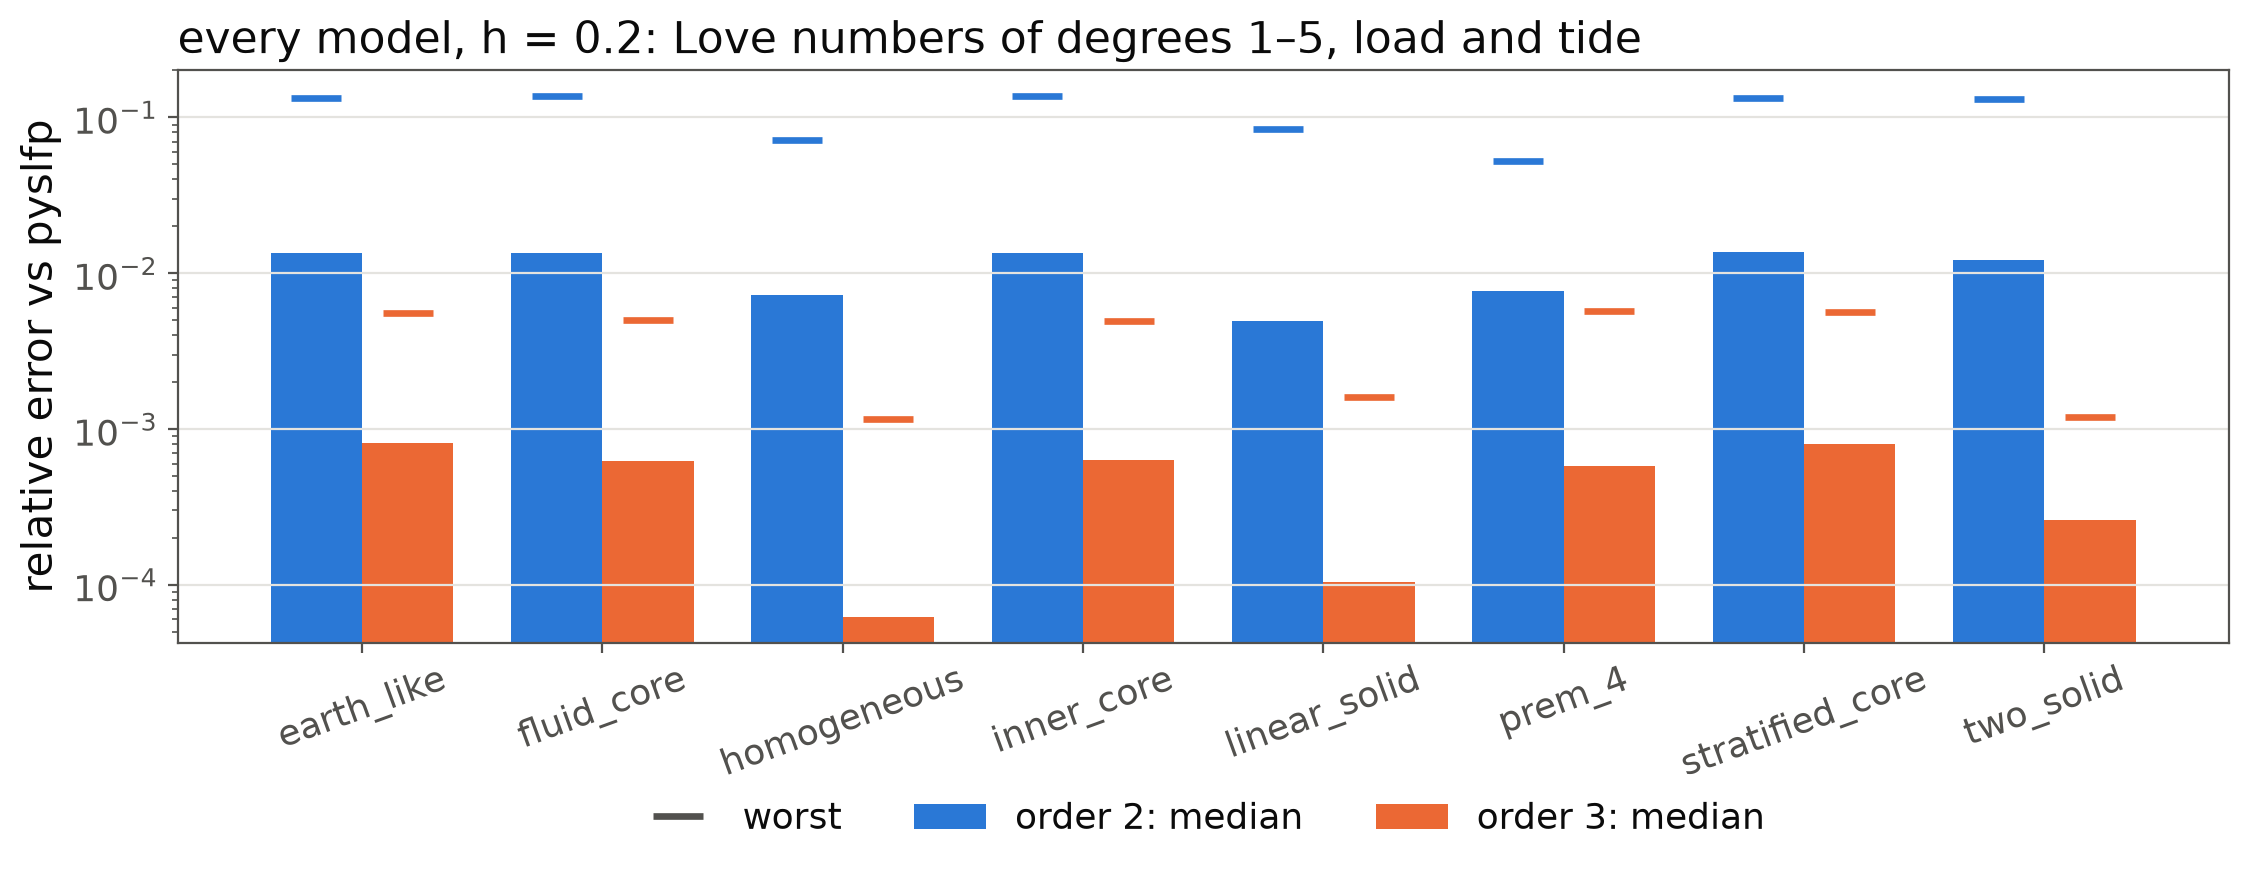
\includegraphics[width=0.92\textwidth]{talk_models.png}
\caption{All-model sweep, $h=0.2$: the median (bar) and the worst
(tick) relative error of the Love numbers of degrees 1--5, load and tide,
at orders 2 and 3. Dahlen path, full CMB treatment. Data of 28 Sep 2026.}
\label{fig:models}
\end{figure}

\paragraph{The $h$-ladder on \code{fluid\_core} (Figures~\ref{fig:ladder}, \ref{fig:conv}).}
Order 2 decreases, irregularly, from 1--2\,\% to 0.2--0.7\,\% between
$h=0.3$ and $0.12$. The fitted rates are 0.6--2.6 depending on the
number, well below the $h^{3}$ one might hope for in a surface functional.
Order 3 is 10--100 times more accurate at every $h$, but between $h=0.3$
and $0.15$ it is flat, sitting on a plateau of a few $10^{-4}$ in most
numbers, and then drops by one to two orders of magnitude at $h=0.12$
alone. The field errors (Figure~\ref{fig:fieldconv}) show the same
plateau-and-noise pattern. The ladder is therefore not in its asymptotic
regime, and its fitted rates should not be read as convergence
orders\review{r:ladder}. The geometry-order-3 ladder
(\code{fluid\_core\_geom3}), which is not plotted, is \emph{less} accurate
at order 3 than geometry order 2 at the same $h$ and shows no drop at
$0.12$, which deserves a look.

\begin{figure}[H]
\centering
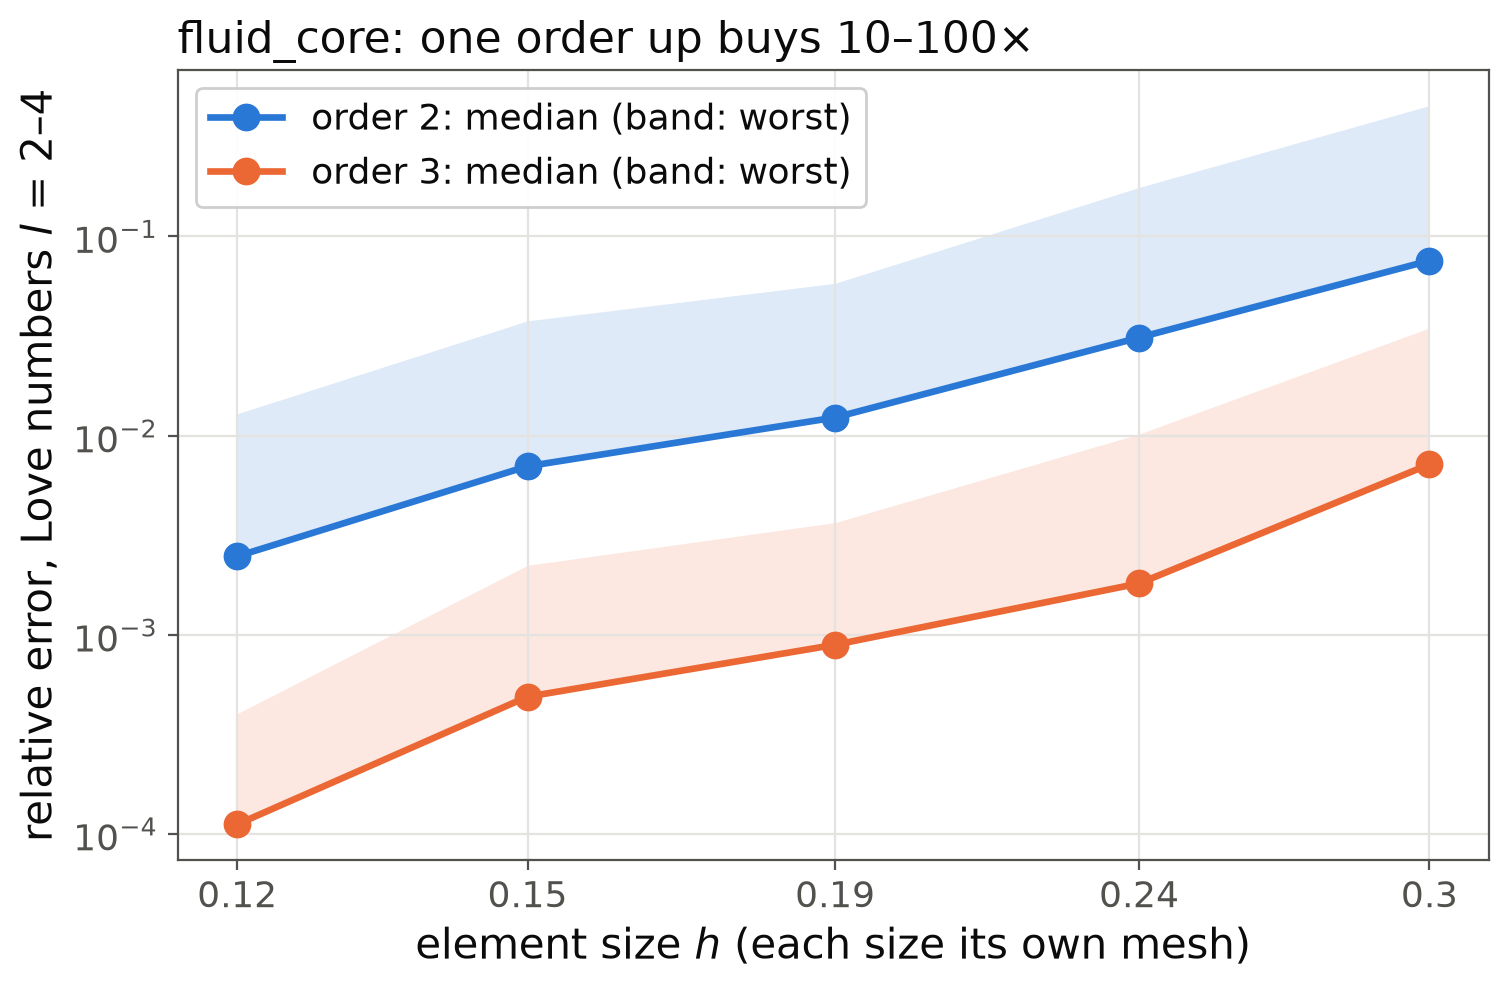
\includegraphics[width=0.6\textwidth]{talk_ladder.png}
\caption{$h$-ladder, \code{fluid\_core}, Dahlen: the median (line) and the
worst (band) relative error of the Love numbers of degrees 2--4.}
\label{fig:ladder}
\end{figure}

\begin{figure}[H]
\centering
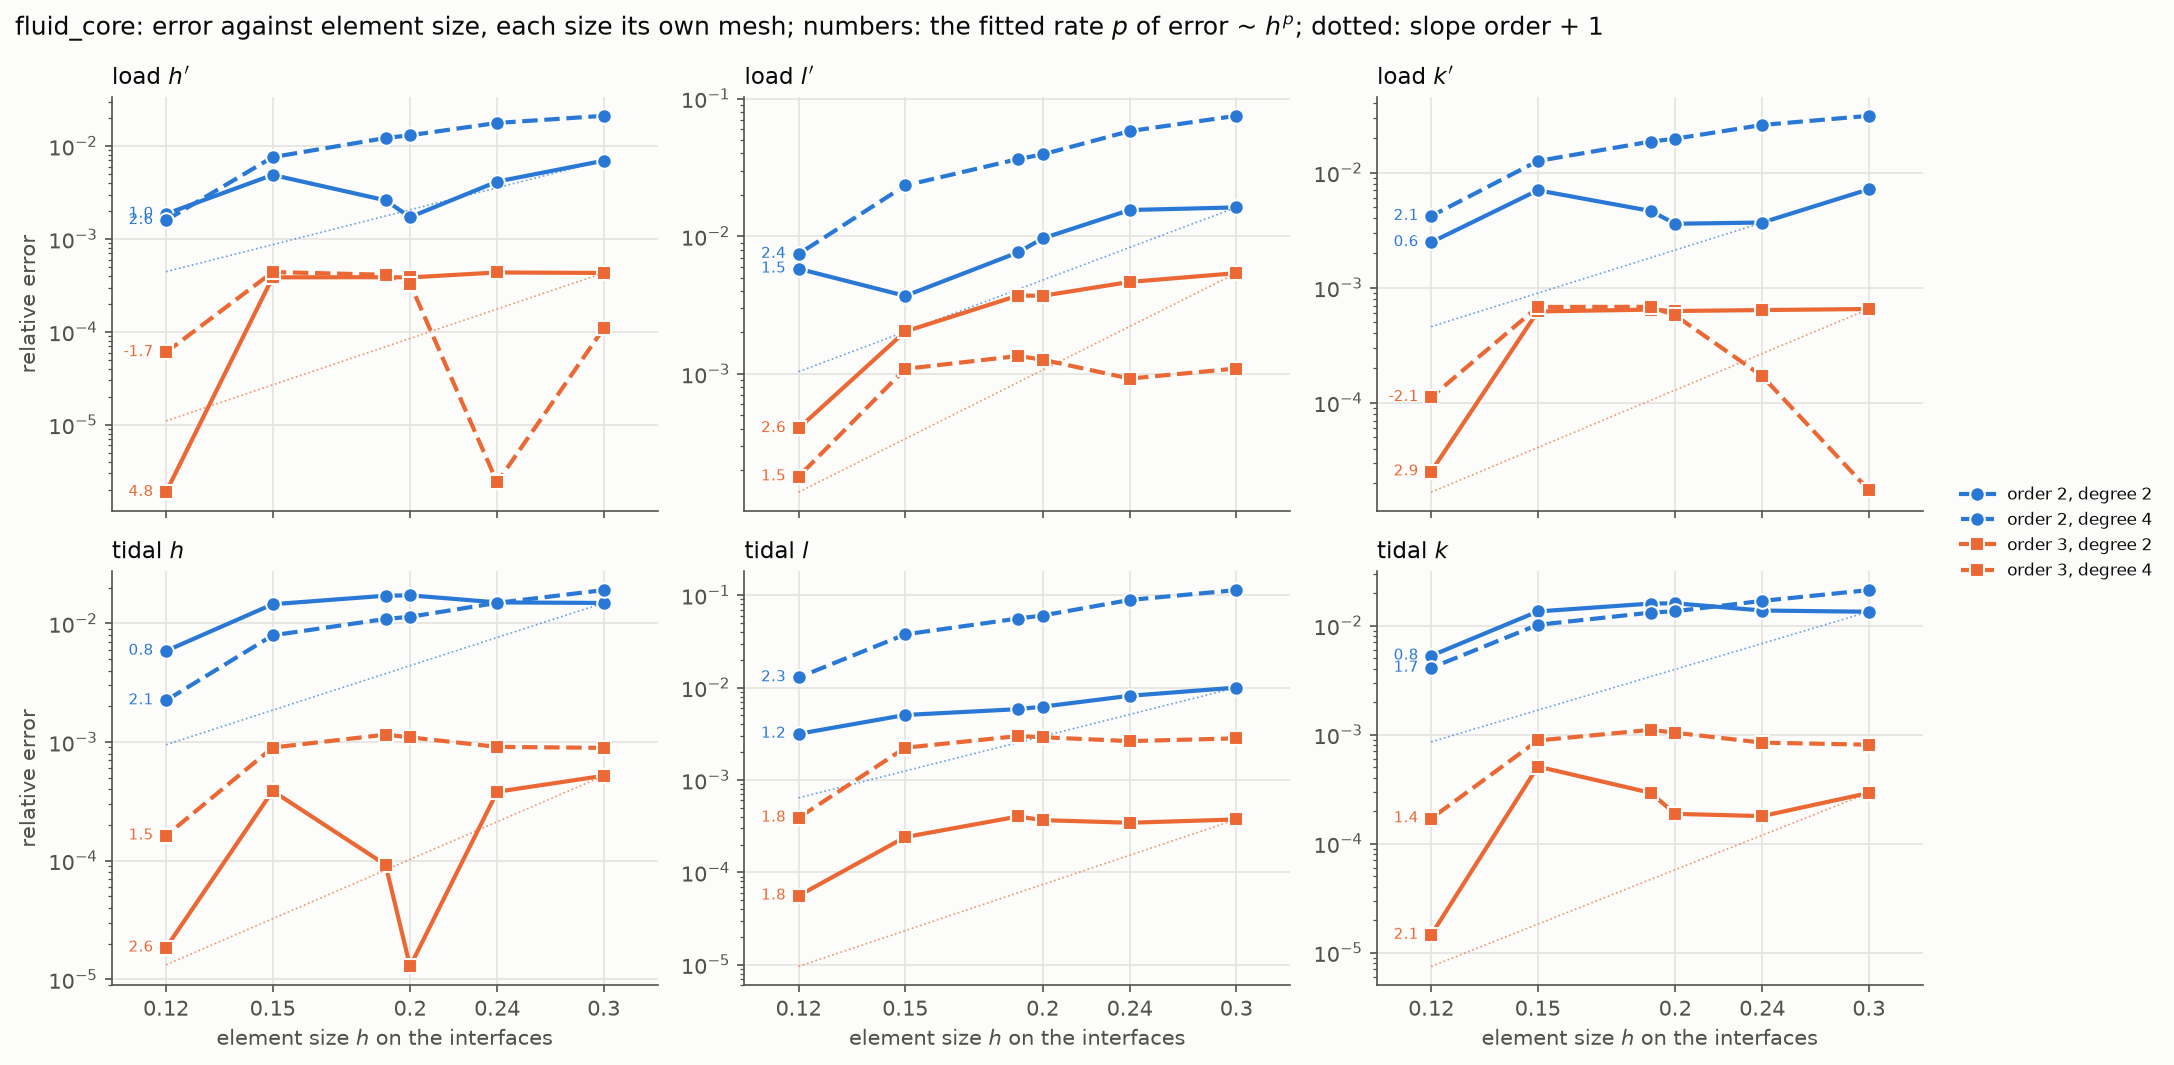
\includegraphics[width=\textwidth]{fc_convergence.png}
\caption{The same ladder number by number: degree 2 solid, degree 4
dashed, the fitted rate beside the finest point, and a guide of slope
$\text{order}+1$ (dotted). Redrawn with the corrected \code{plot.py}.}
\label{fig:conv}
\end{figure}

\begin{figure}[H]
\centering
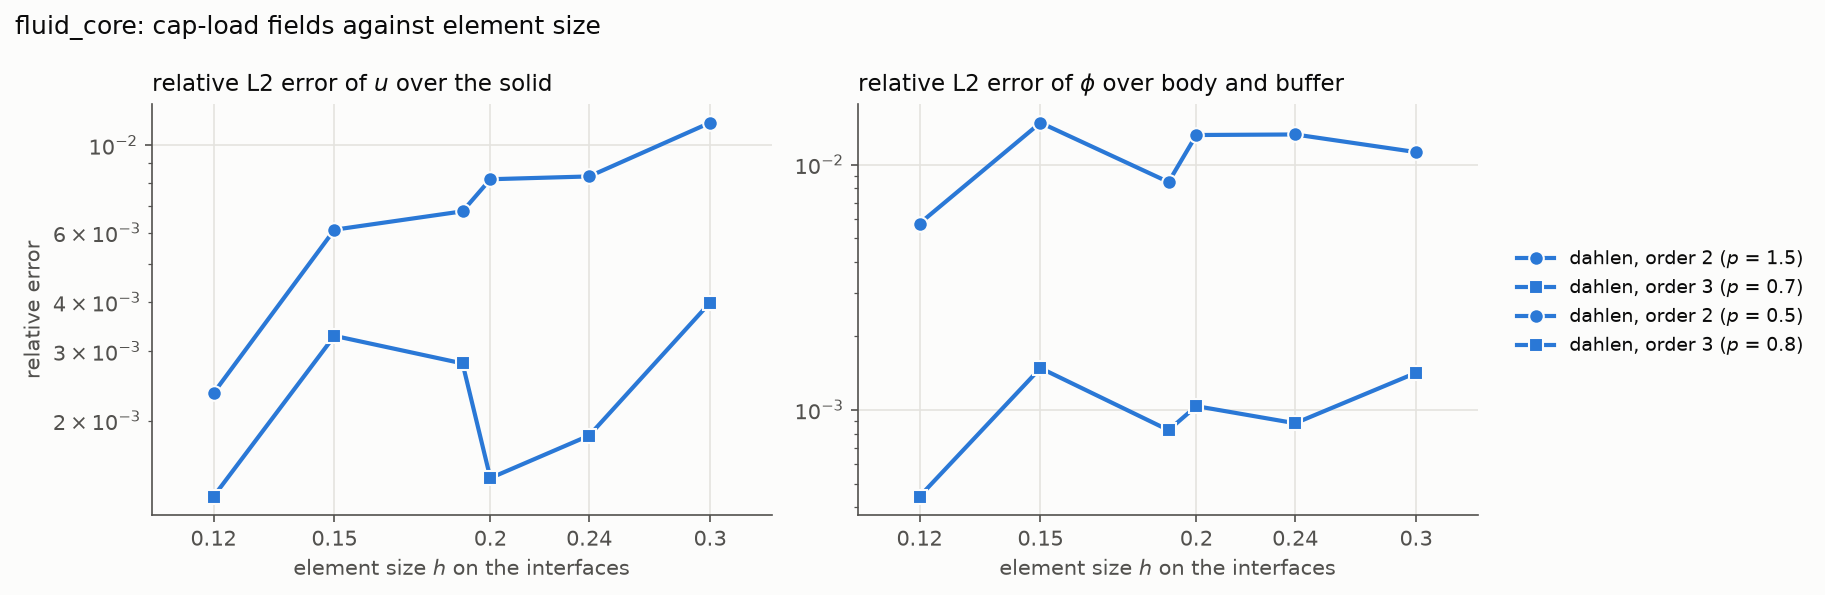
\includegraphics[width=0.75\textwidth]{fc_field_convergence.png}
\caption{The cap-load fields against $h$ on the same ladder.}
\label{fig:fieldconv}
\end{figure}

\begin{figure}[H]
\centering
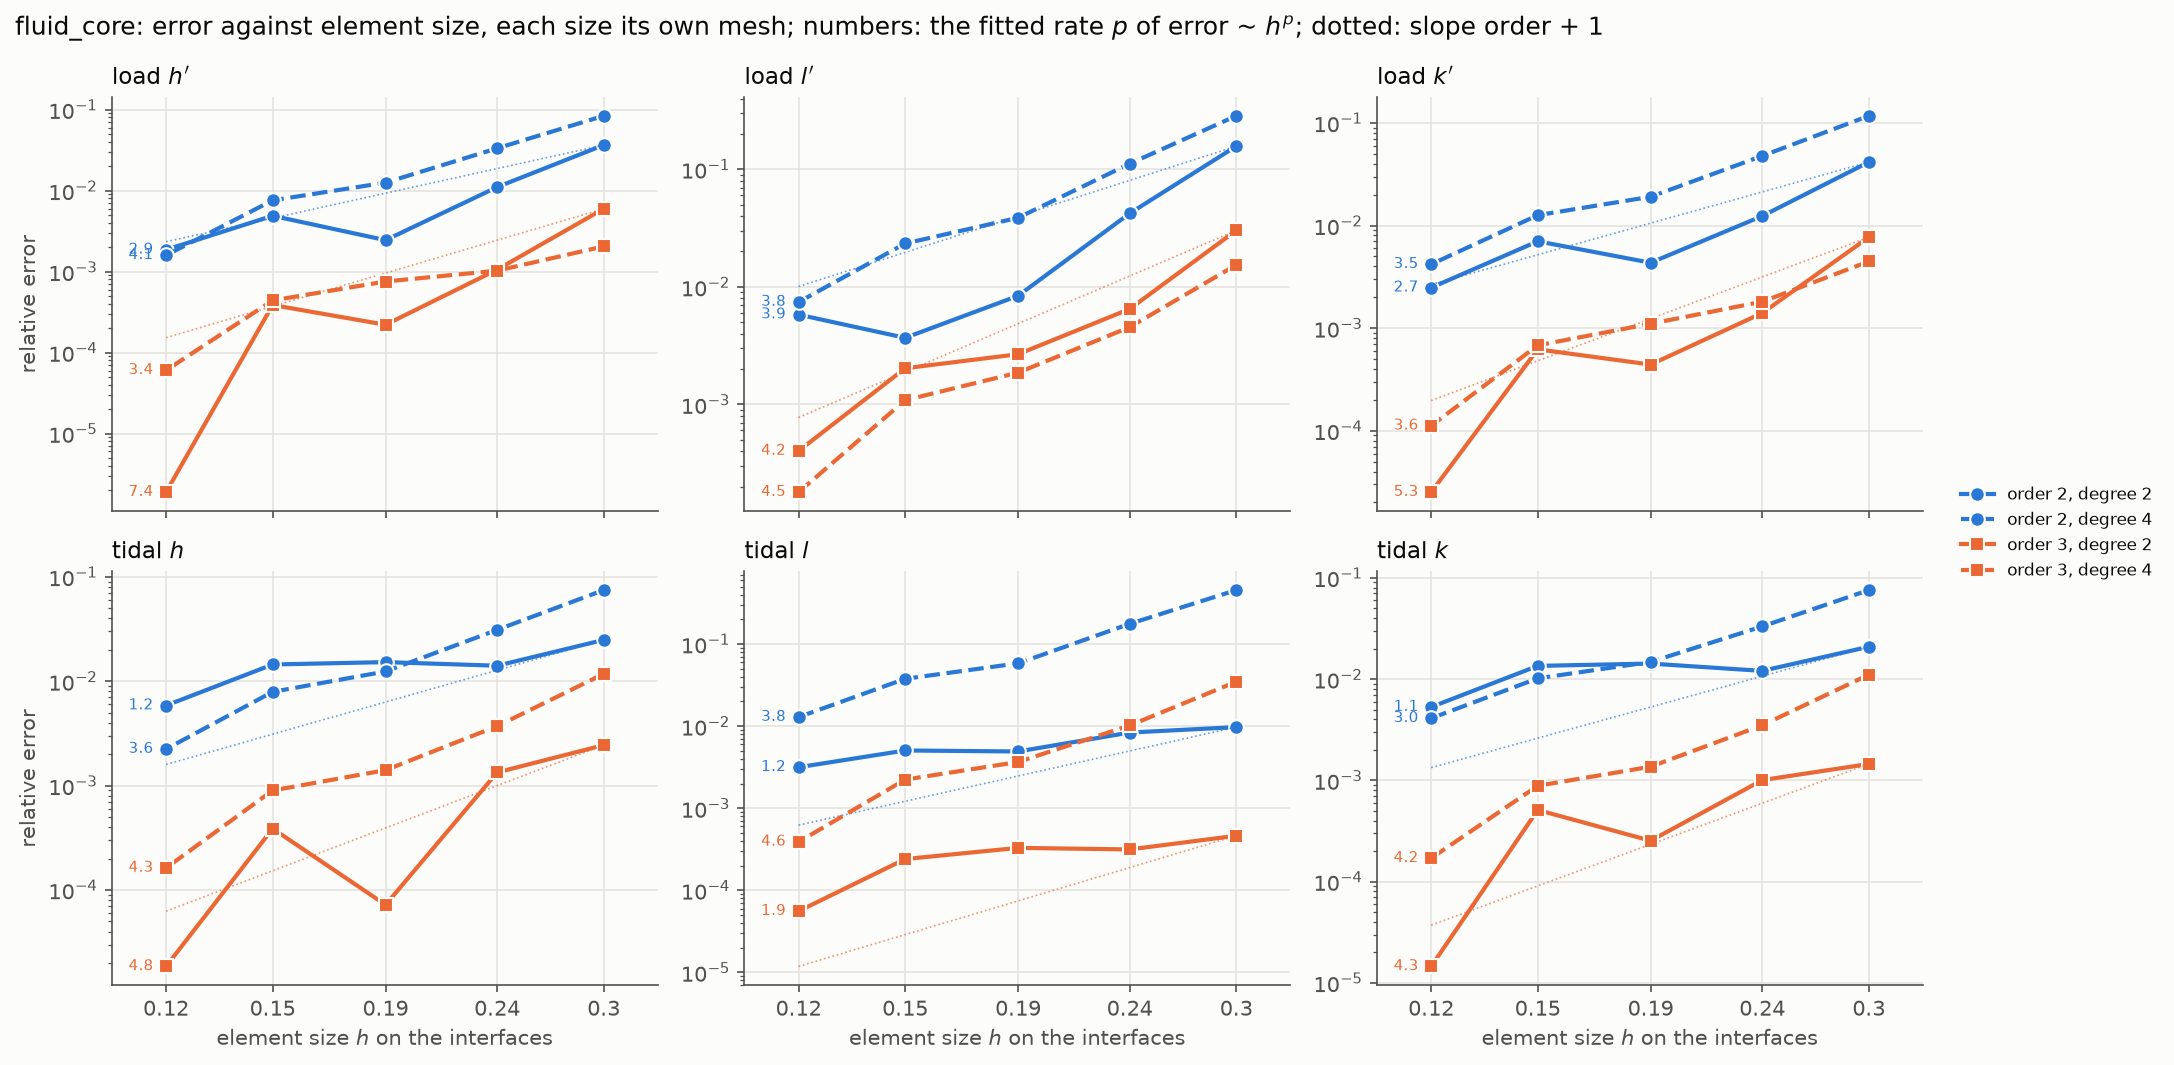
\includegraphics[width=\textwidth]{fc_convergence_uncapped.png}
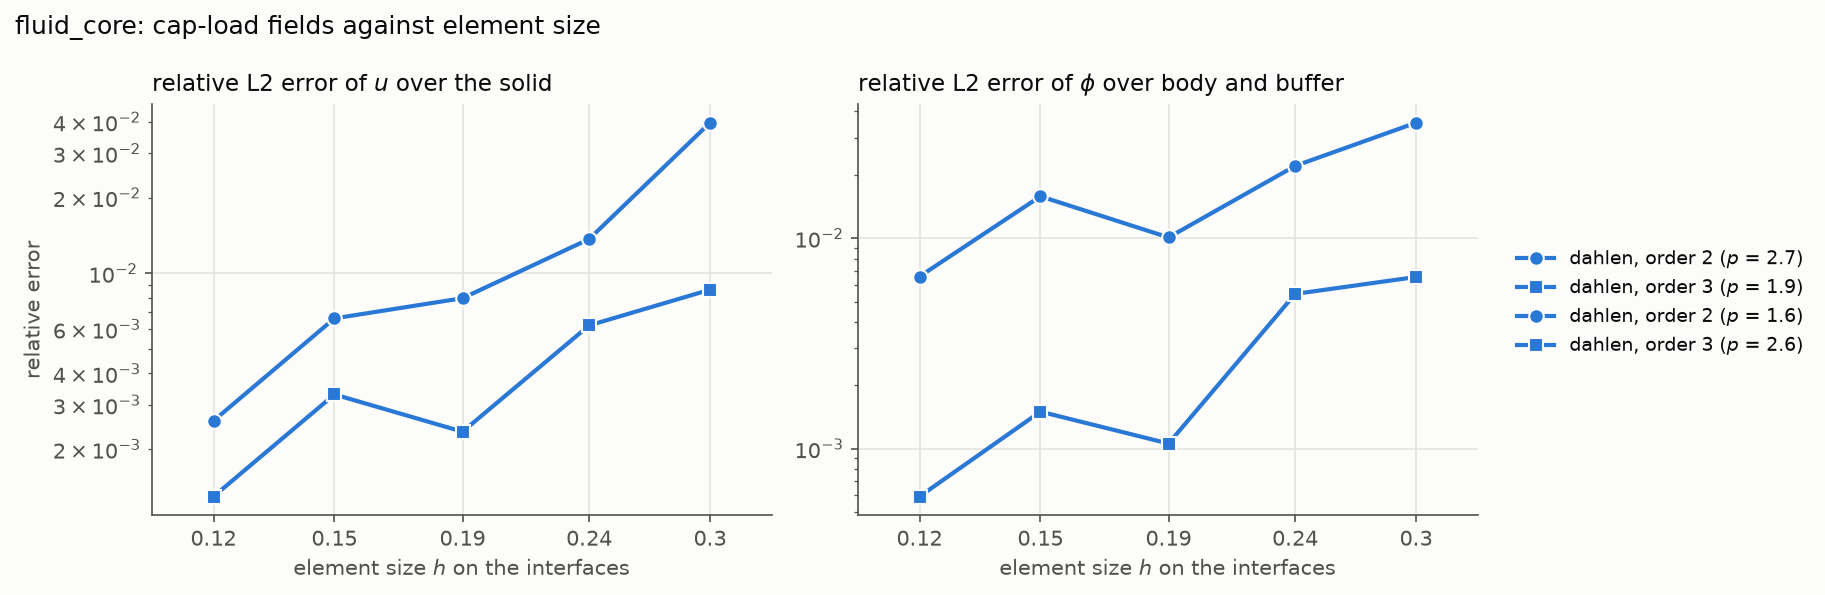
\includegraphics[width=0.75\textwidth]{fc_field_convergence_uncapped.png}
\caption{The UNCAPPED ladder (2 Oct, \ref{r:ladder}'s rerun:
\code{--angular 1.0}, so every rung refines the CMB; current code,
\code{runs\_campaign/ladder}). The order-3 flat-then-cliff of
Figure~\ref{fig:conv} is gone and the field errors fall throughout;
the Love-number columns still carry cancellation (the implied degree-2
rate is superconvergent), so the field rates are the quotable ones.}
\label{fig:convuncapped}
\end{figure}

\paragraph{Cross-method comparison (Figures~\ref{fig:methods}--\ref{fig:timing}).}
On \code{fluid\_core}, $h=0.3$, order 2, every formulation agrees with
pyslfp to 0.2--4\,\% in $h'$ and $k'$ at degrees 0--4, which is the
discretisation level at this resolution. The gauged and compressible
formulations also agree at $l=0$, where Dahlen does not by design. The
spread between methods is mesh error, not a difference in physics. The
$l'$ column is larger in relative terms ($l'_2$ is small), and
\code{winkler} is the outlier (\S\ref{sec:cmbresults}). Cost differs much
more than accuracy: per load solve, Dahlen takes about 1\,s (117
iterations), gauged about 5--9\,s (780), referential about 7--12\,s (810),
slip 40--75\,s (2300--3000) and slip\_broken 45--110\,s (4700--6300),
depending on the run (Figure~\ref{fig:timing}; the talk figure uses the
30 Sep sweep).

\begin{figure}[H]
\centering
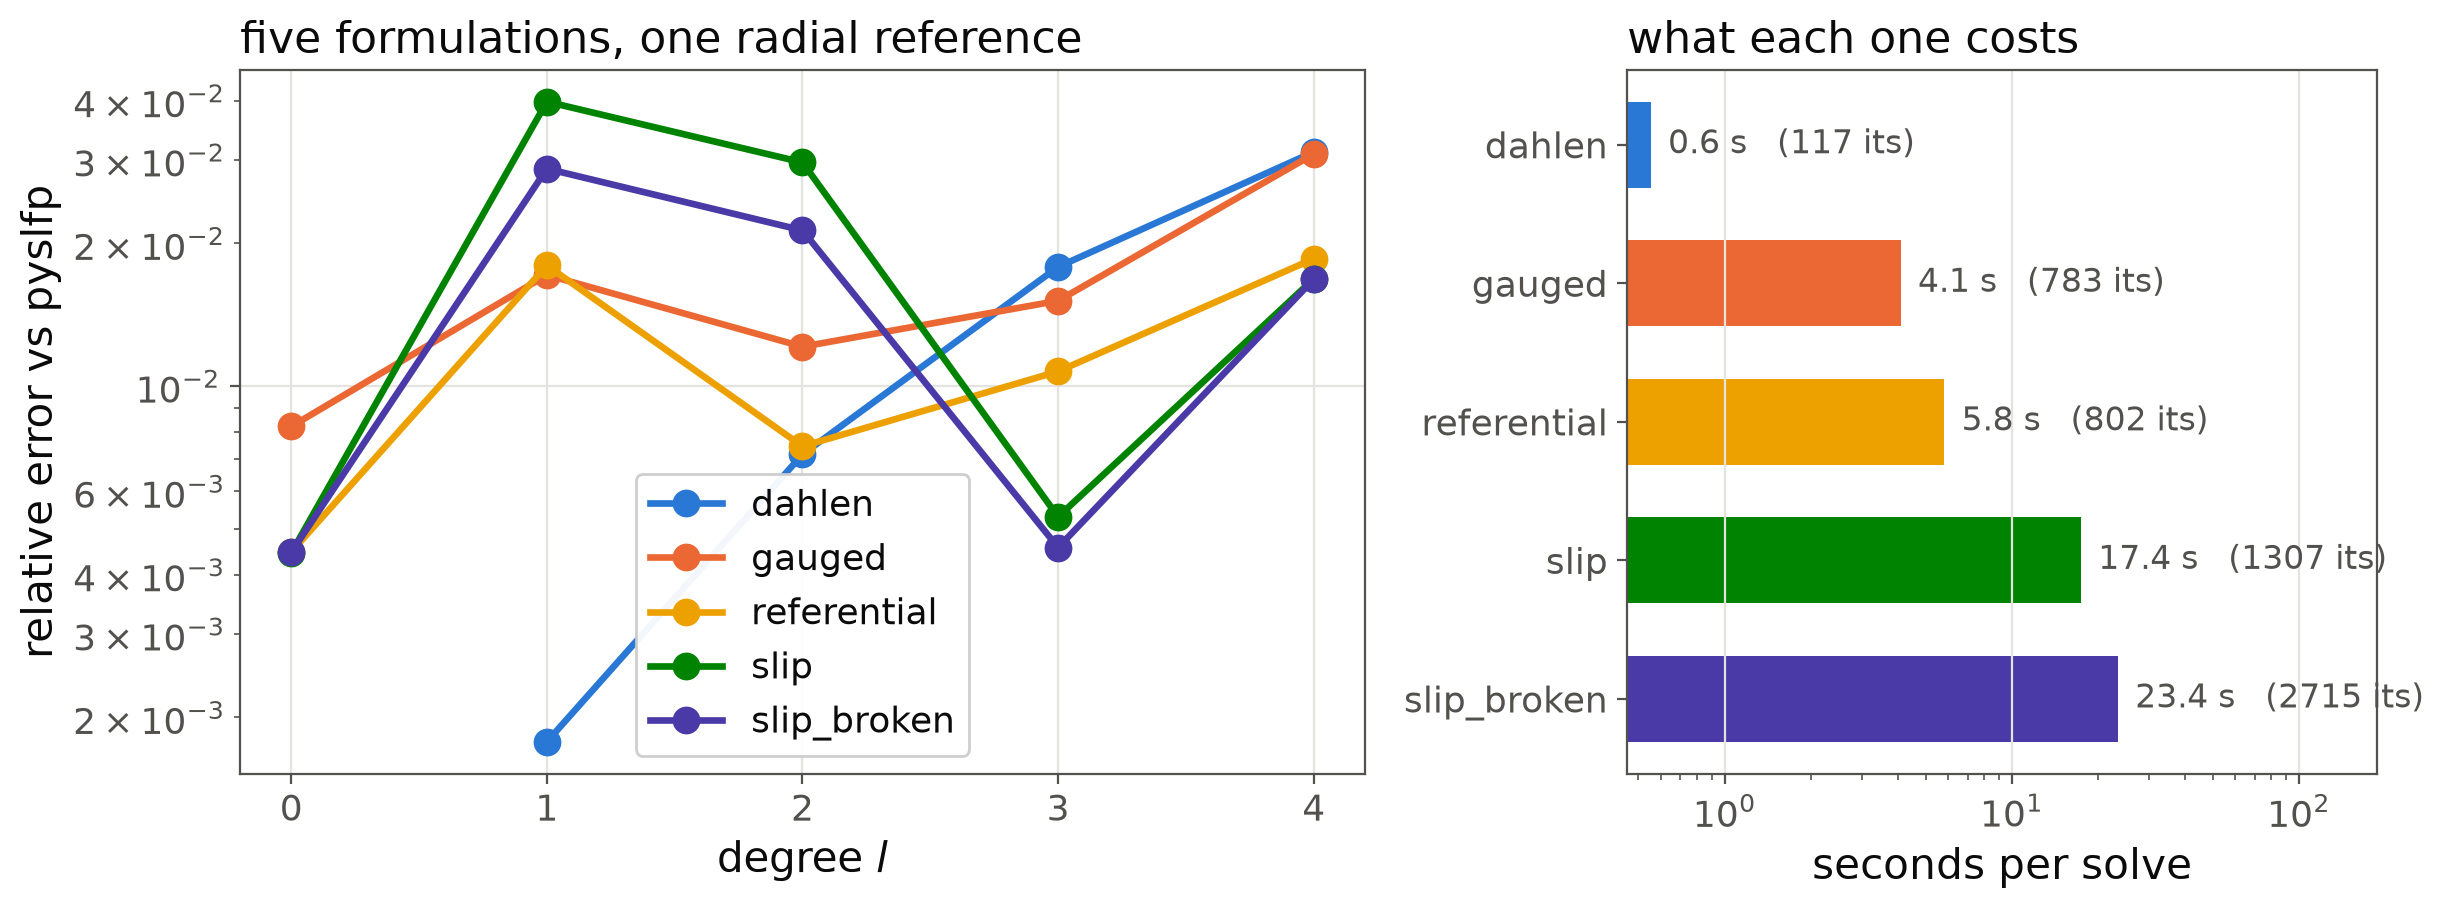
\includegraphics[width=0.95\textwidth]{talk_methods.png}
\caption{Talk figure: the five formulations on one case
(\code{fluid\_core}, $h=0.3$, order 2), worst of $h'$, $k'$ per degree, and
the mean cost per load solve.}
\label{fig:methods}
\end{figure}

\begin{figure}[H]
\centering
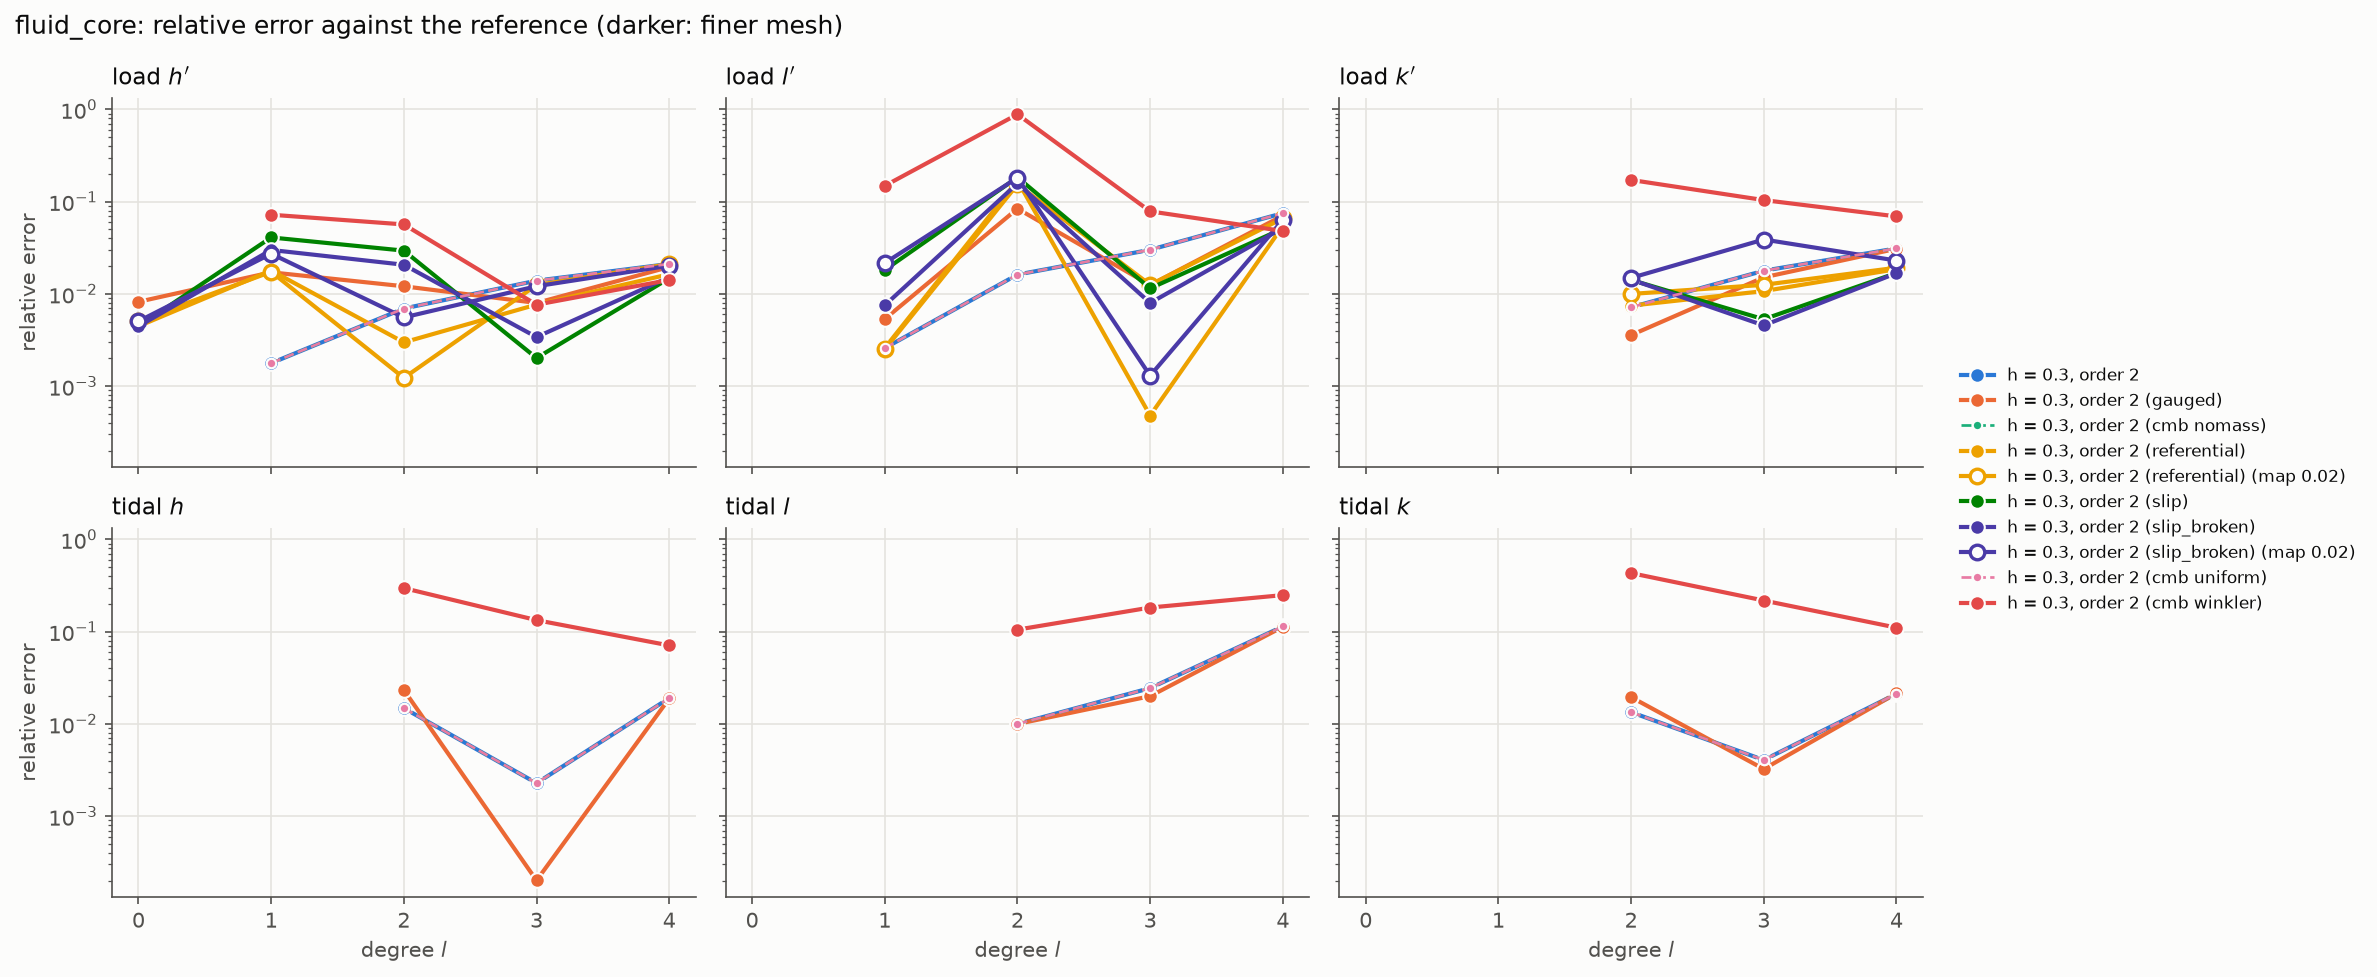
\includegraphics[width=\textwidth]{fc_errors.png}
\caption{Every variant run on \code{fluid\_core}, $h=0.3$, order 2
(1 Oct campaign). One colour per formulation or CMB treatment, the same
in every figure. Mapped runs are hollow. \code{nomass} and \code{uniform}
are drawn thin and dashed, since on this uniform core they lie on top
of the full treatment.}
\label{fig:errors}
\end{figure}

\begin{figure}[H]
\centering
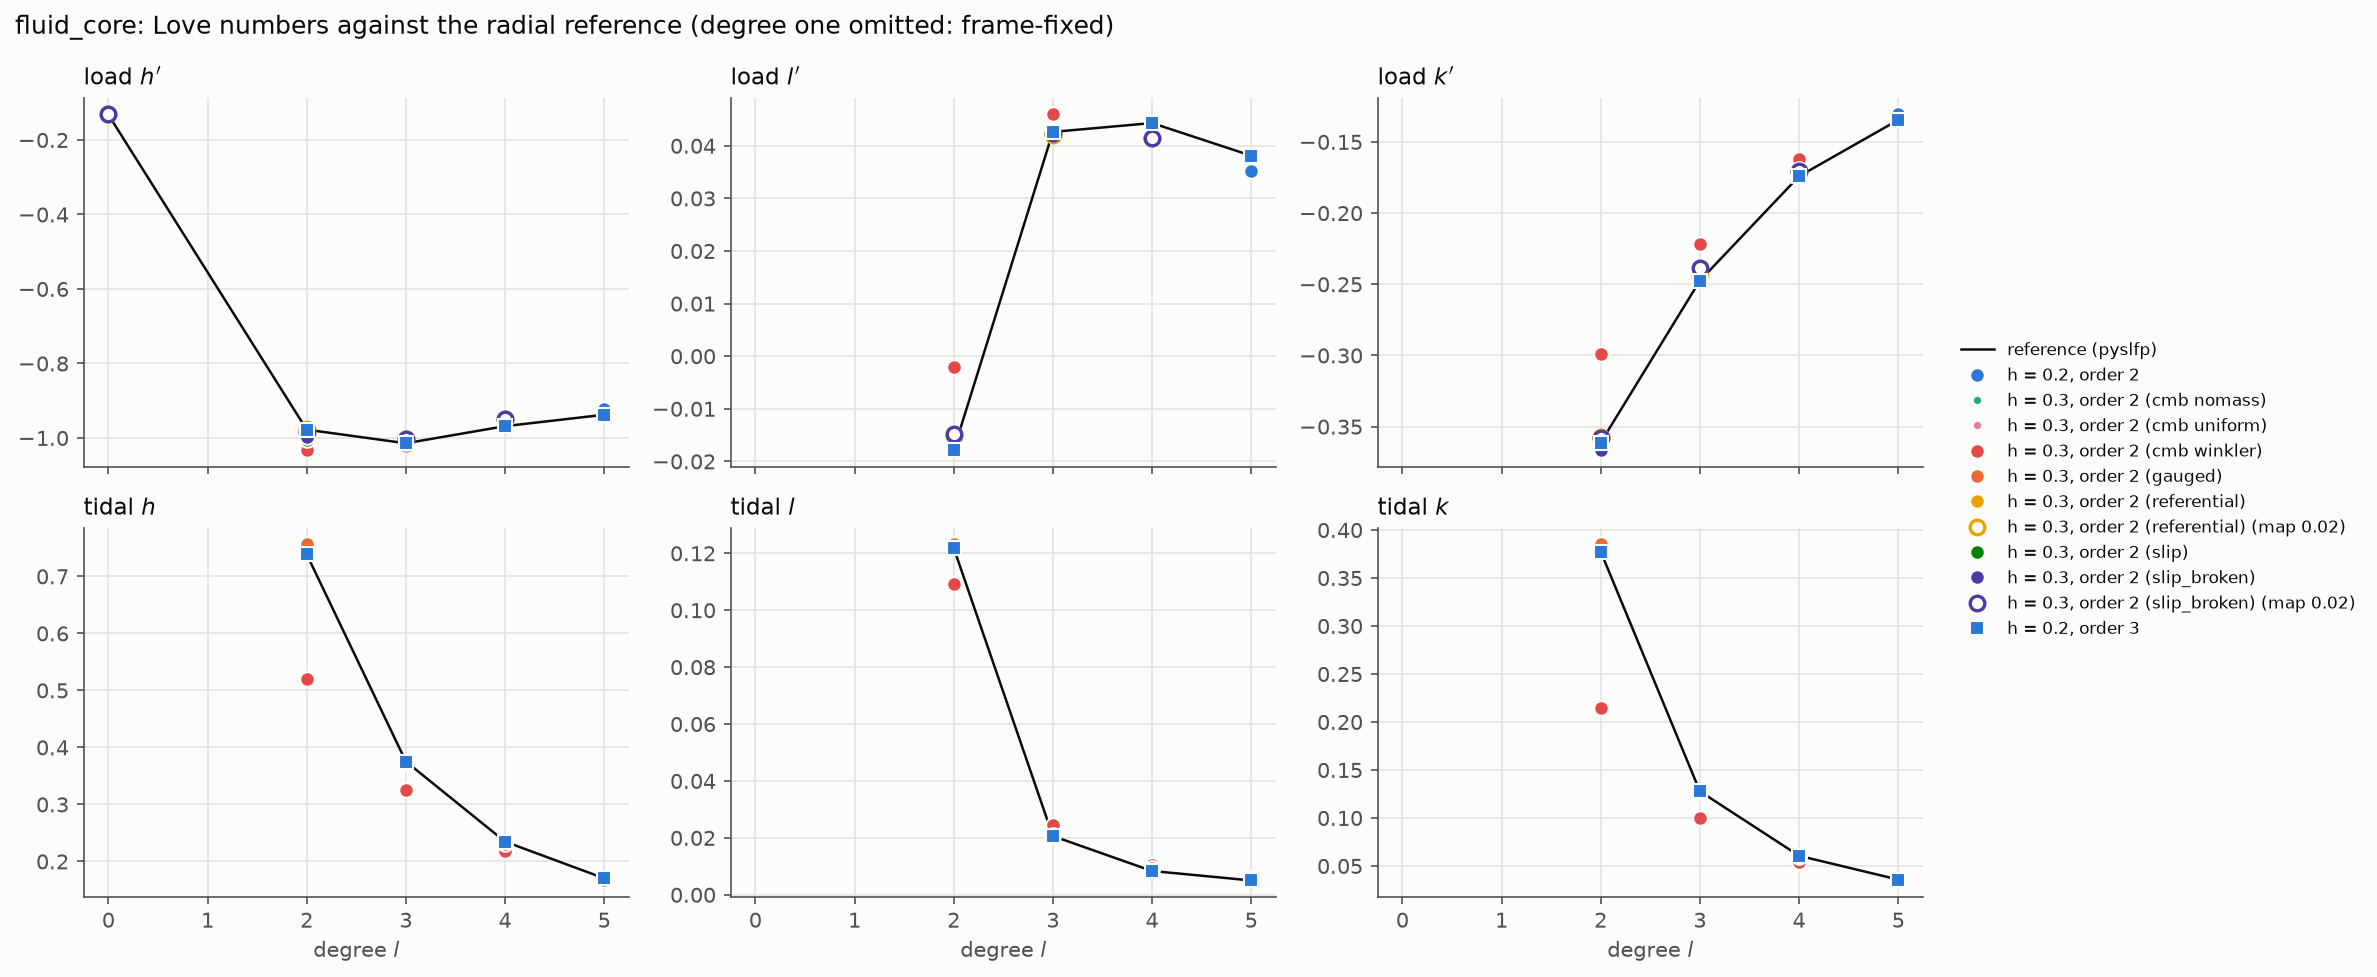
\includegraphics[width=\textwidth]{fc_love_numbers.png}
\caption{The Love numbers themselves against the reference.}
\label{fig:lovenumbers}
\end{figure}

\begin{figure}[H]
\centering
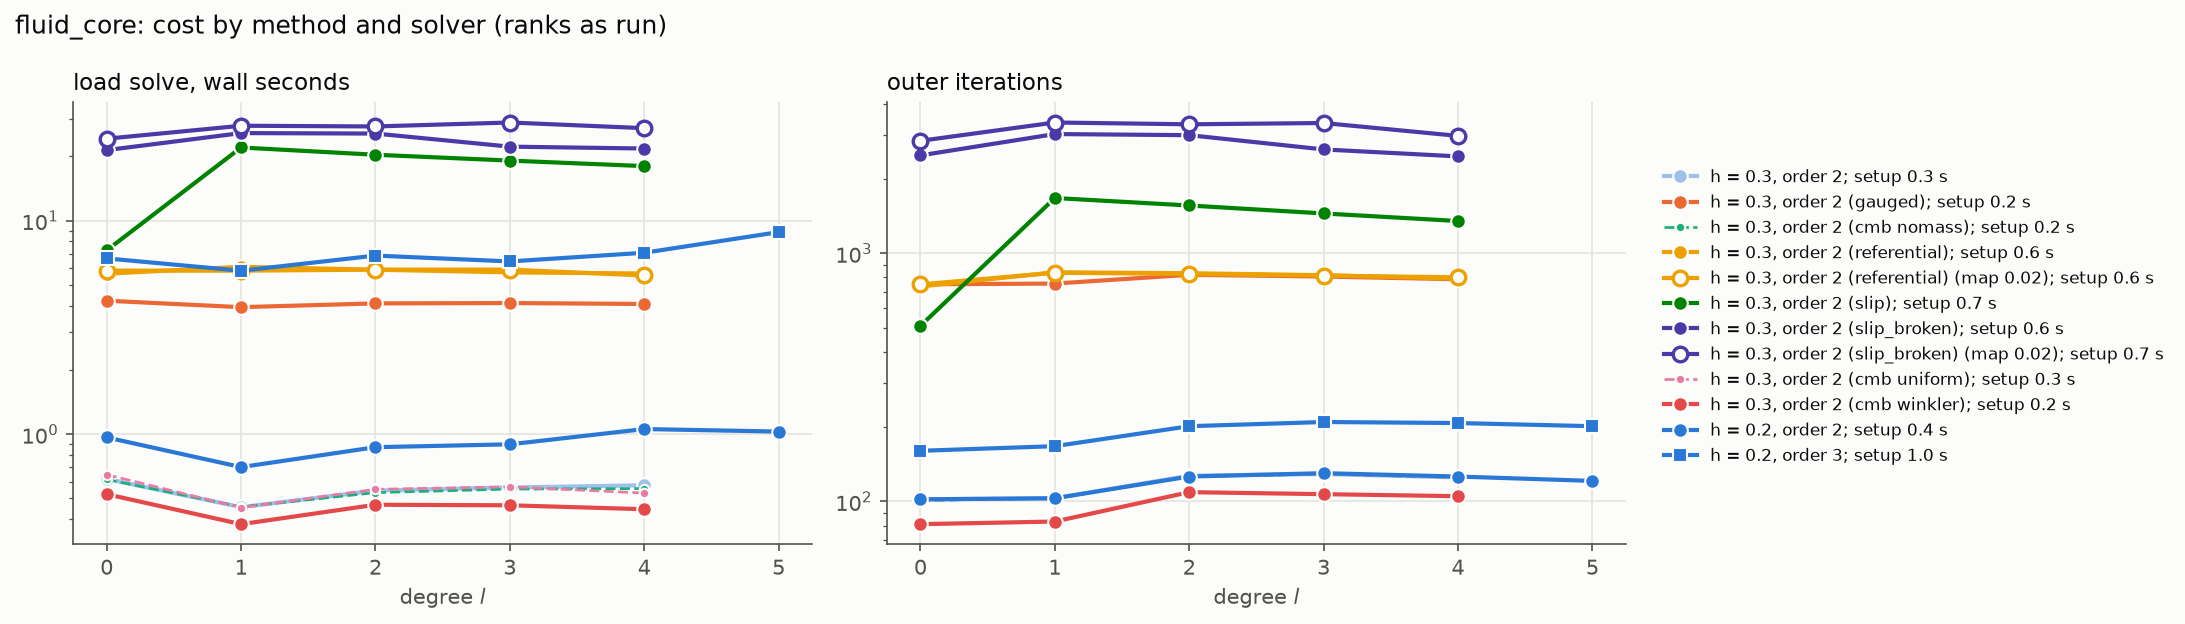
\includegraphics[width=0.95\textwidth]{fc_timing.png}
\caption{Cost per load solve by degree: wall seconds and outer
iterations (logarithmic).}
\label{fig:timing}
\end{figure}

\paragraph{Radial profiles (Figure~\ref{fig:profiles}).}
The fitted radial functions \eqref{eq:radialfit} of the Eulerian runs lie
on pyslfp's in every layer and continue harmonically into the buffer.
Two departures are visible: \code{winkler}, by design, and the gauged
$\phi_1$ inside the fluid core, which bends away from the reference
below $r\approx 0.5$ while matching at the interfaces. The second may be
a frame or gauge effect in the profile fit rather than an error of the
solution, but it is not explained anywhere\review{r:gaugedprofile}.

\begin{figure}[H]
\centering
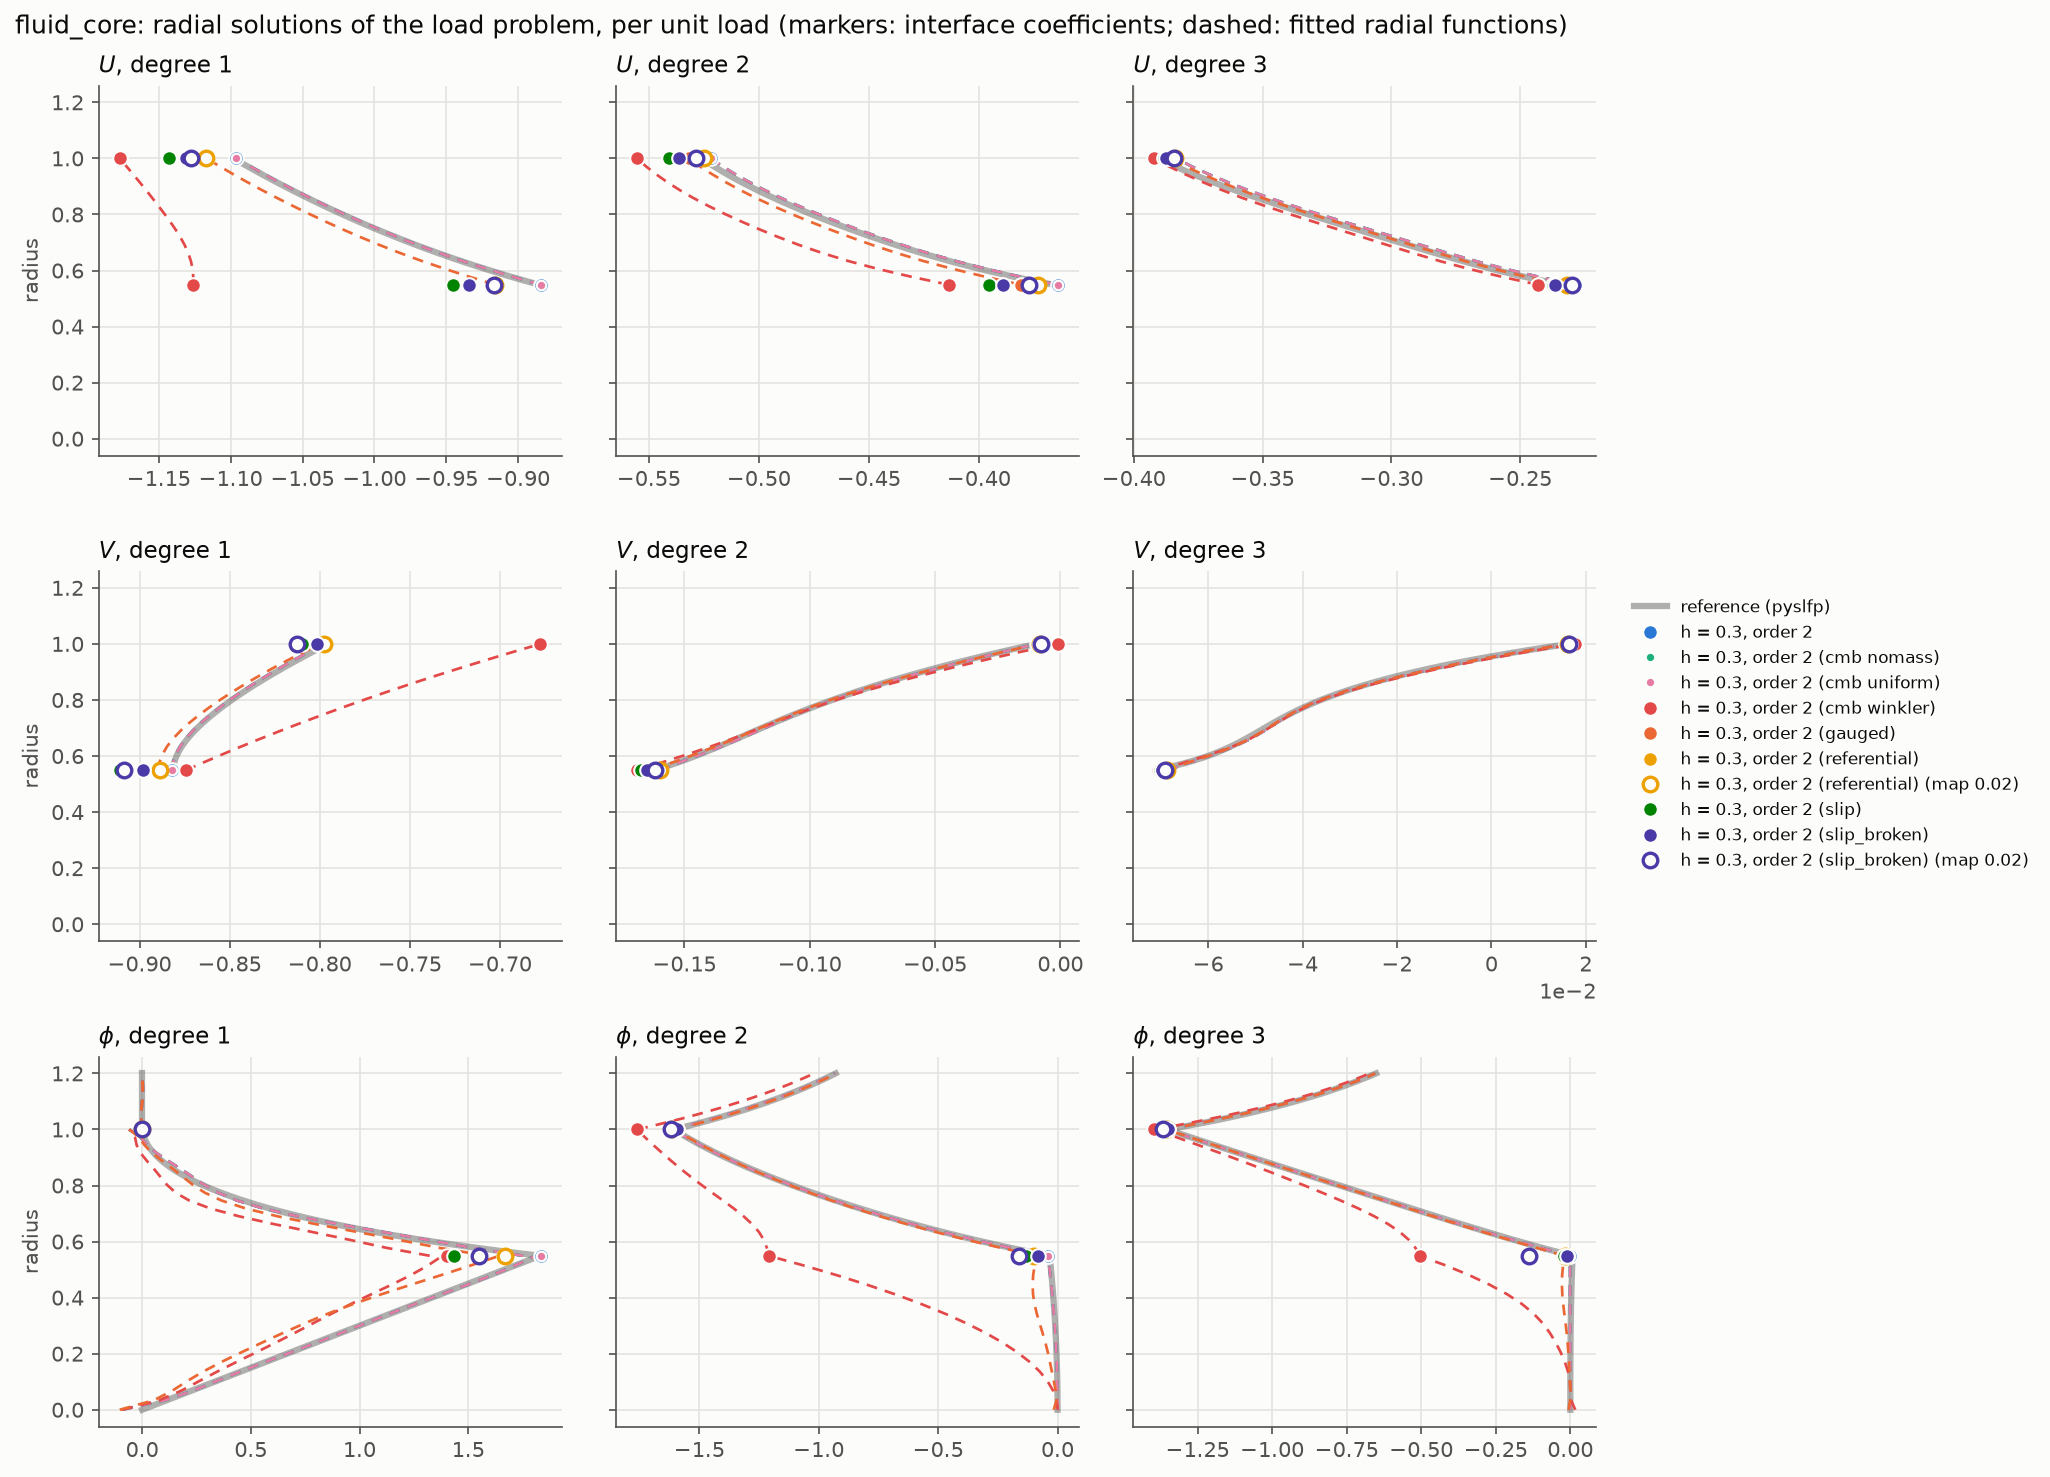
\includegraphics[width=0.9\textwidth]{fc_profiles.png}
\caption{Radial functions of the load problem, degrees 1--3: reference
(grey), fitted FE radial functions (dashed) and interface coefficients
(markers). Only the Eulerian methods write profiles.}
\label{fig:profiles}
\end{figure}

\paragraph{Fields (Figures~\ref{fig:fieldmap}, \ref{fig:spectrum}).}
On \code{fluid\_core}, $h=0.3$, order 2, Dahlen, the relative $L^2$ errors
are $1.3\times10^{-2}$ ($\vu$) and $1.4\times10^{-2}$ ($\phi$). The
pointwise difference of the radial displacement on the surface is at most
2.7\,\% of the signal and concentrates under the cap edge. By degree, the
surface error grows steadily from about $10^{-2}$ at $l=2$ to $10^{-1}$
($U$) and $5\times10^{-1}$ ($V$) at $l=8$. That is the resolution limit
of $h=0.3$, about 1/8 of a degree-8 wavelength per element. The gauged
run's $\vu$ error of 0.40 is not a property of the solution: the norm
includes the fluid core, where the reference displacement is set to zero
\review{r:gaugedfield}.

\begin{figure}[H]
\centering
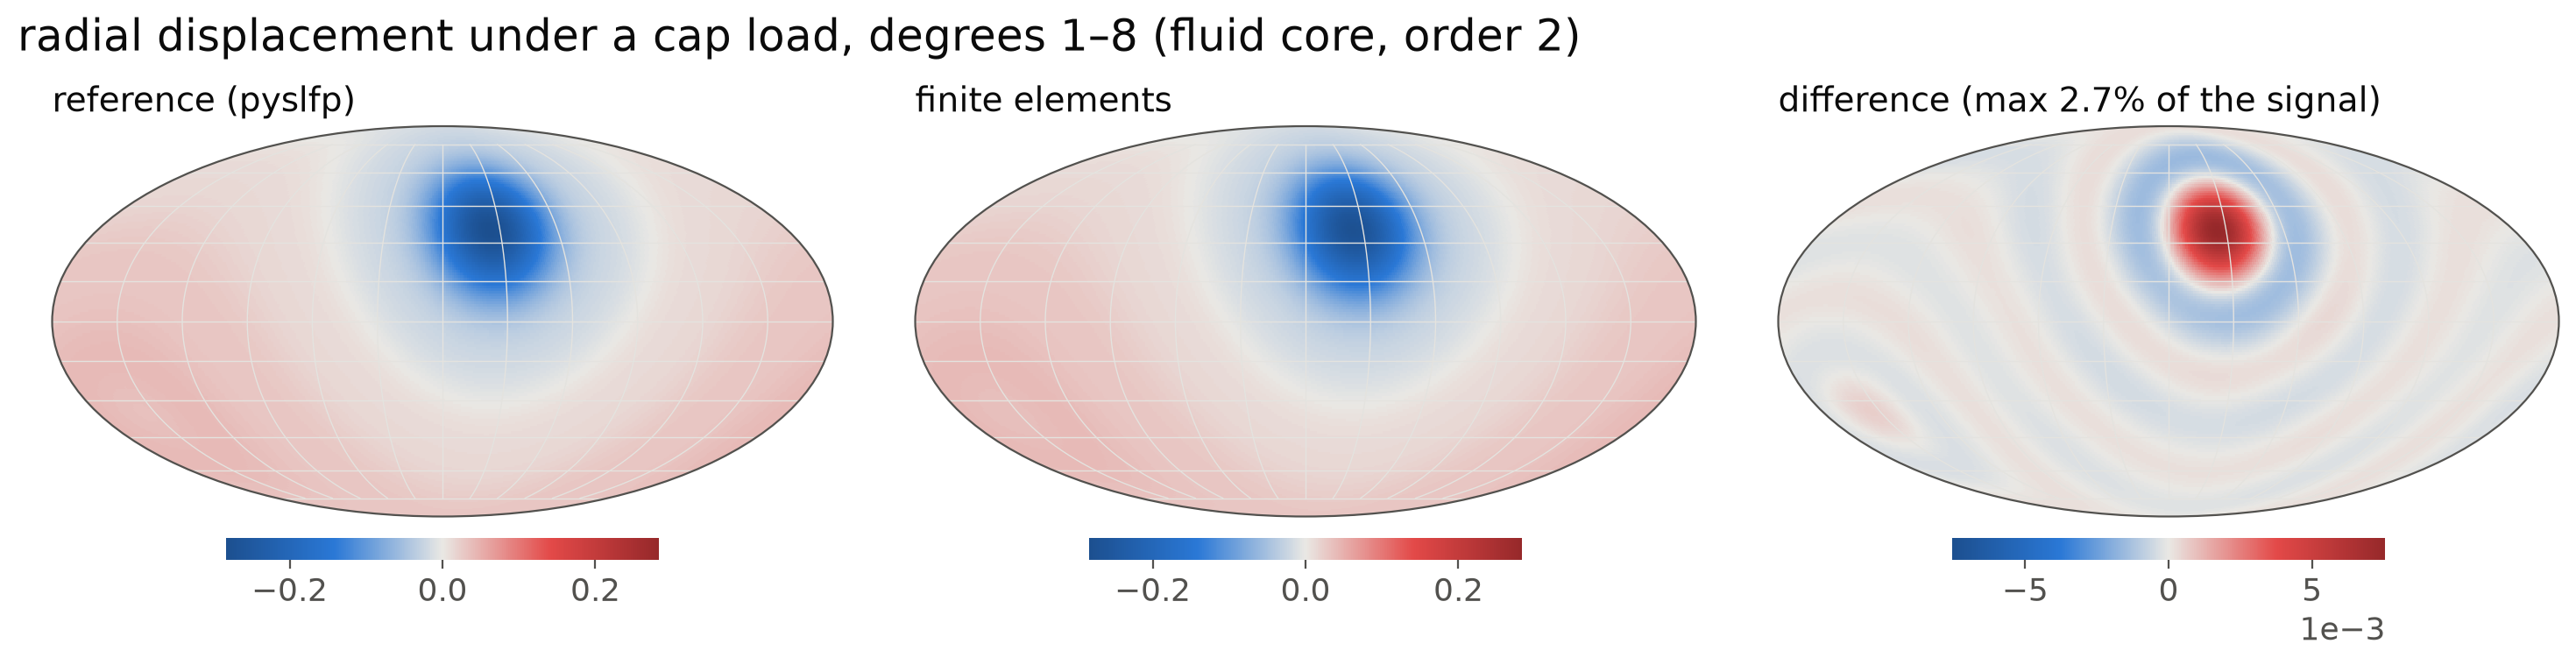
\includegraphics[width=\textwidth]{talk_fieldmap.png}
\caption{Radial displacement on the surface under the cap load
(\code{fluid\_core}, Dahlen, order 2): reference, FE, and their difference
on its own scale.}
\label{fig:fieldmap}
\end{figure}

\begin{figure}[H]
\centering
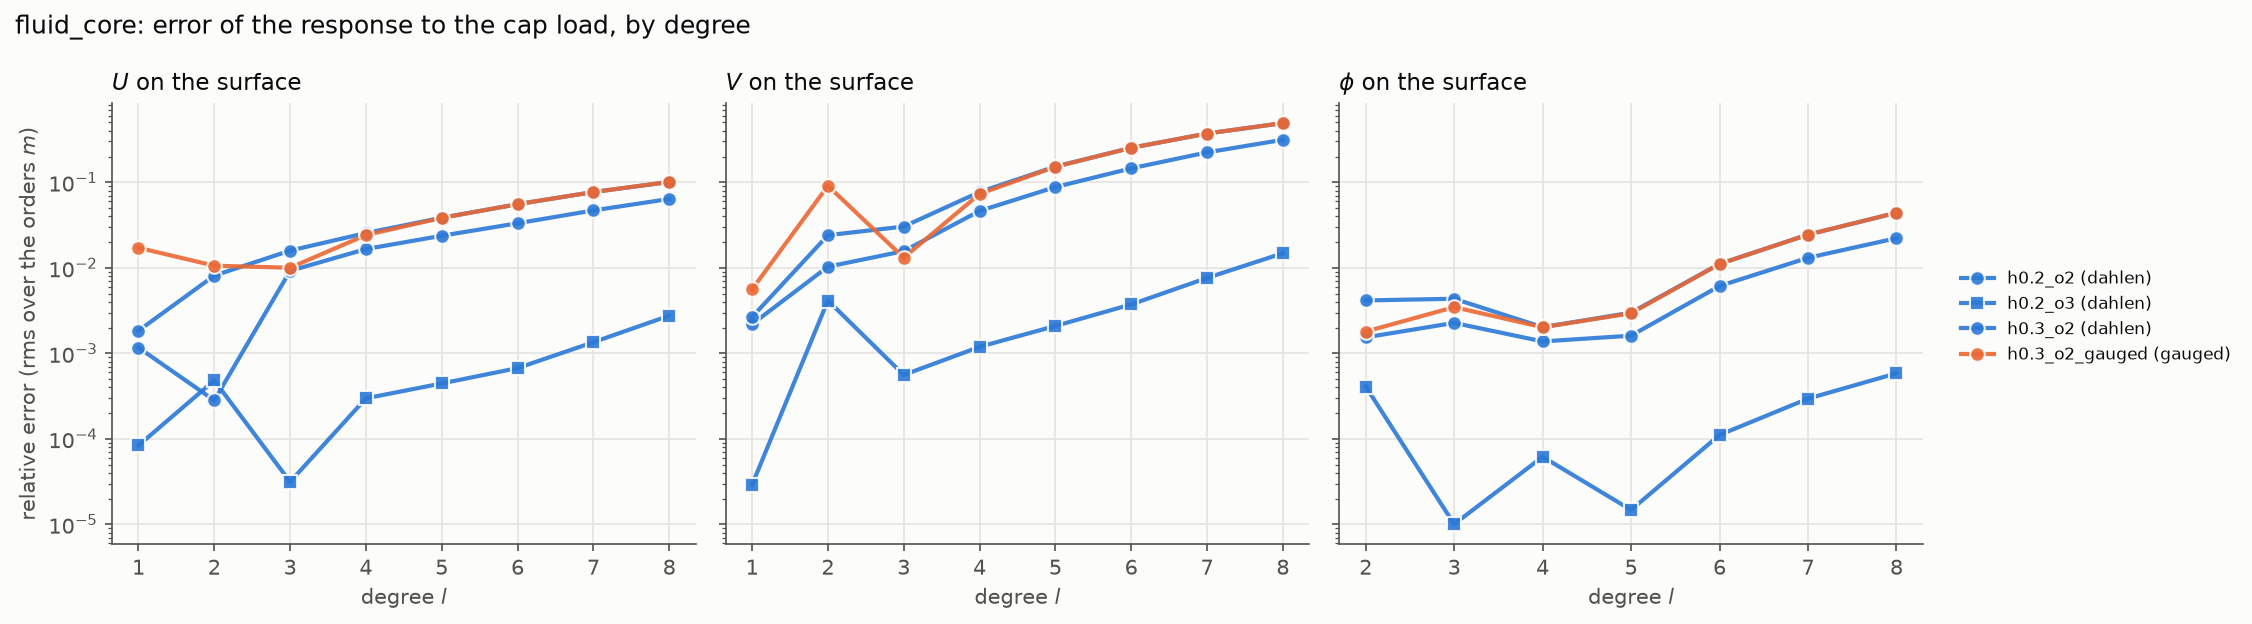
\includegraphics[width=\textwidth]{fc_field_spectrum.png}
\caption{Cap load: root-mean-square relative error of the surface
coefficients by degree. $\phi$ at degree one is omitted because it is
zero in both solutions by the choice of frame.}
\label{fig:spectrum}
\end{figure}

\subsection{The CMB approximations: results}
\label{sec:cmbresults}

On \code{prem\_4\_cmb} ($h=0.2$, order 2), the deviation from the full
treatment, which is the approximation error alone, is:
\begin{center}
\small
\begin{tabular}{@{}lcccccc@{}}
\toprule
 & load $h'_2$ & load $l'_2$ & load $k'_2$ & tidal $h_2$ & tidal $l_2$ & tidal $k_2$ \\
\midrule
\code{nomass}, \code{uniform} & $7.8\times10^{-4}$ & $3.0\times10^{-3}$ & $2.9\times10^{-3}$ & $1.1\times10^{-2}$ & $7.2\times10^{-3}$ & $2.5\times10^{-2}$ \\
\code{winkler} & $7.9\times10^{-2}$ & $0.80$ & $0.14$ & $0.28$ & $3.1\times10^{-2}$ & $0.42$ \\
\bottomrule
\end{tabular}
\end{center}
These approximations are loading-safe at $l\ge 2$: the deviation is below
the discretisation error of the full treatment, about 1\,\% in $k'_2$
here. They are about ten times worse for tides, whose degree-2 response
drives the rotational feedbacks. \code{winkler} (no potential coupling)
is not acceptable for either\review{r:cmbclaim}. On \code{fluid\_core} the
CMB report confirms \code{nomass} $\equiv$ \code{uniform} $\equiv$
\code{full} to $4\times10^{-11}$, with \code{winkler} at 88\,\% in $l'_2$
and 17\,\% in $k'_2$, and \code{winkler} running about 17\,\% fewer
iterations.

\begin{figure}[H]
\centering
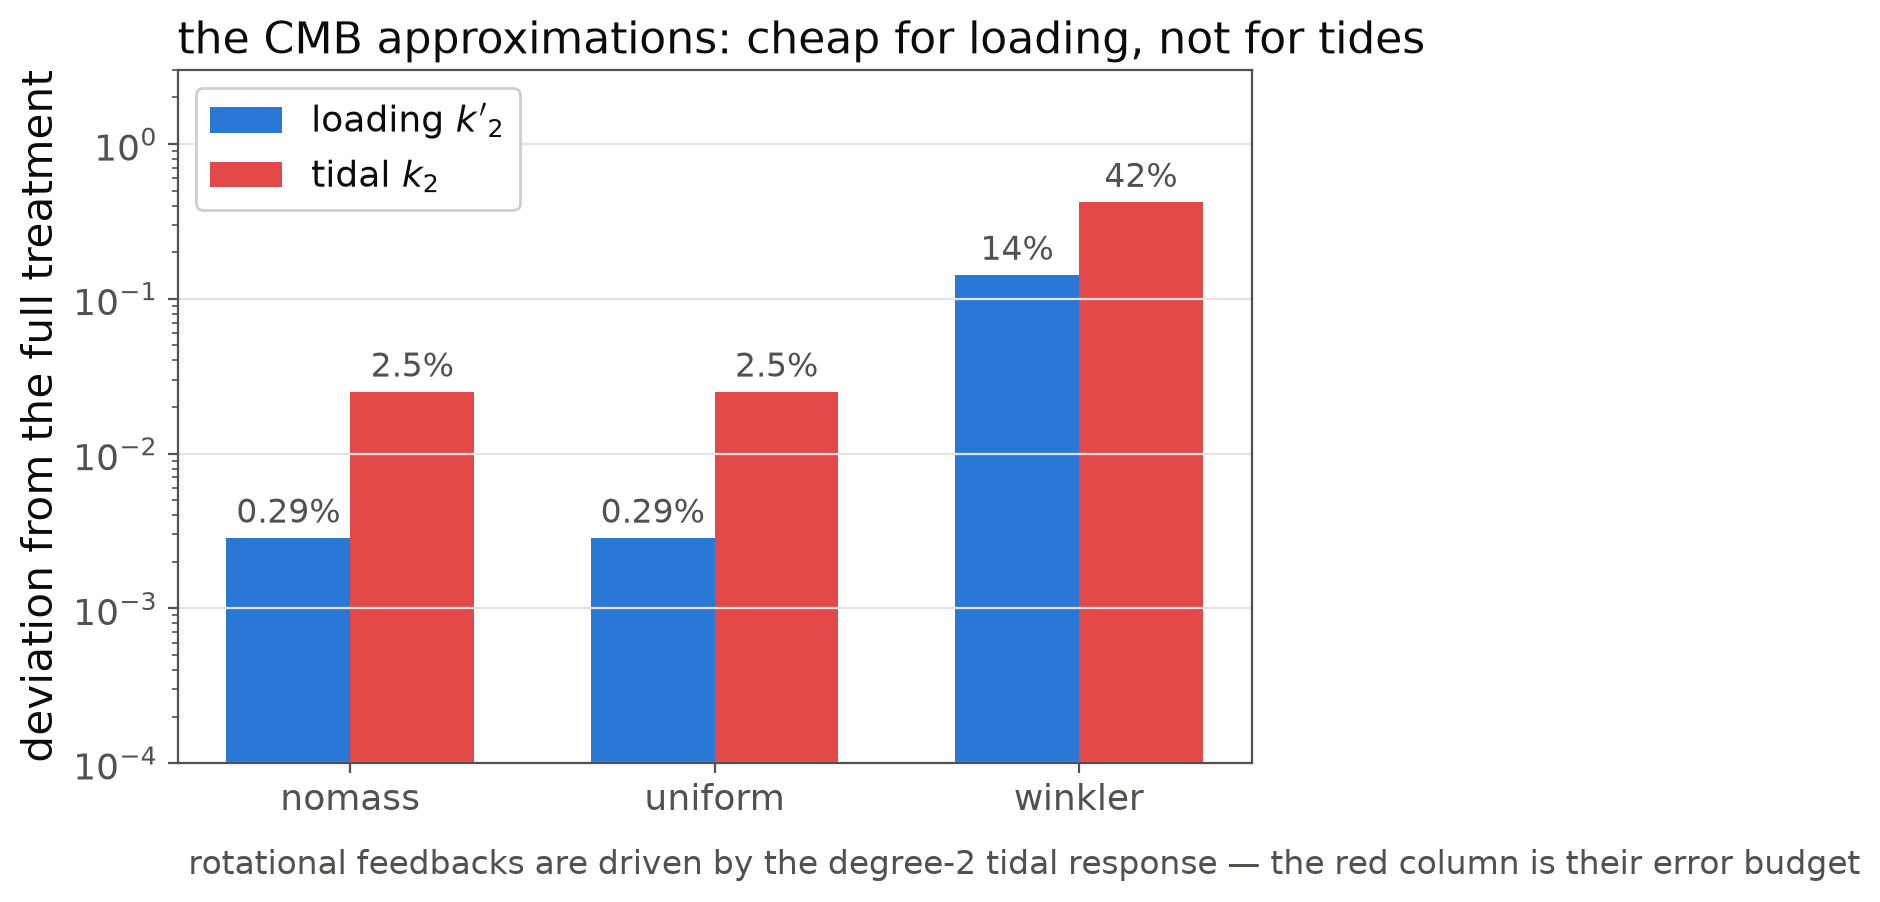
\includegraphics[width=0.7\textwidth]{talk_cmb.png}
\caption{Talk figure: deviation of the CMB approximations from the full
treatment, loading $k'_2$ against tidal $k_2$ (\code{prem\_4}, $h=0.2$,
order 2).}
\end{figure}

%=============================================================================
\section{The relabelling family}
\label{sec:relabel}
%=============================================================================

\subsection{What is tested, and the aim}

The referential classes accept a mapping $\xi$ (a diffeomorphism of the
computational ball onto the physical domain). They assemble every term
pulled back to the reference domain, which is how aspherical bodies and
topography will enter. The relabelling family checks this machinery
\emph{without new physics}, by describing the same spherical problem in
relabelled coordinates. pyslfp then stays an exact reference while every
mapped code path is exercised. With $F=\partial\xi/\partial\vx$ and
$J=\det F$, the pulled-back forms (\code{doc/mappings.md}) are
\begin{equation}
  \int\tilde\nabla\tilde\phi\cdot\tilde\nabla\tilde\phi' \,\mathrm{d}\xi
     = \int J\,C^{-1}\nabla\phi\cdot\nabla\phi'\dV,\quad C=F^TF,
  \qquad
  c'_{iAkB} = J\,c_{ijkl}F^{-1}_{Aj}F^{-1}_{Bl},
\end{equation}
mass-type terms take a factor $J$ (so the density is $\rho J$),
gradient couplings take $F^{-T}$, and boundary terms use Nanson's
relation $\tilde\vm\,\mathrm{d}\tilde S = J F^{-T}\vn\dS$. The coefficients
are the physical fields composed with $\xi$, $\rho(\vx)=\tilde\rho(\xi(\vx))$
and similarly for the others. The family has three legs, which differ in
how $F$ is known and in what is compared.

\subsection{The interior relabelling}

The map of legs A and B is
\begin{equation}
  \xi(\vx) = \vx + A\sum_{i}h_i(r)\,\mathbf{w}(\vx),\qquad
  h_i(r) = \Bigl[\frac{4(r-r_i)(r_{i+1}-r)}{(r_{i+1}-r_i)^2}\Bigr]^2
  \ \ (r_i<r<r_{i+1}),
  \label{eq:relabel}
\end{equation}
\begin{equation*}
  \mathbf{w} = \bigl(\sin\pi y + c\cos\pi z,\ \sin\pi z + c\cos\pi x,\
               \sin\pi x + c\cos\pi y\bigr),\qquad c=\tfrac12 ,
\end{equation*}
with $h_i$ a bump on each body layer $[r_i,r_{i+1}]$ that vanishes with its
first derivative at the layer's boundaries. So $\xi$ is the identity, with
$F=I$, on every interface and on and outside the surface, and it is fully
three-dimensional in between. The physical problem is therefore the
spherical one: interfaces, surface and DtN sphere are untouched, so the
harmonic analysis needs no change. The pulled-back coefficients carry
full lateral variation, and the pulled-back elastic tensor loses its
minor symmetries. The driver checks that the map is the identity on the
outer sphere to $10^{-12}$ and on the interfaces to $10^{-6}$, the facets'
geometric error squared. Benchmark amplitude: $A=0.02$.

\subsection{Leg A: mapped Love numbers (\code{love\_benchmark -map})}

\textbf{Test.} The referential and slip\_broken methods are solved with
the exact analytic $\xi$ and $F$, and with coefficients from the exact
radial profiles composed with $\xi$ (the $L^2$ fields cannot be evaluated
at $|\xi(\vx)|$). The Love numbers must reproduce pyslfp's to the
discretisation level, plus the geometric floor. The single-valued slip
refuses maps by design, and the Eulerian classes are unmapped.
\textbf{Measured} (1 Oct campaign, $h=0.3$): the mapped and unmapped
runs differ by at most $2.4\times10^{-3}$ (\code{homogeneous}),
$3.5\times10^{-2}$ (\code{two\_solid}, in $l'_4$) and $1.5\times10^{-2}$
(\code{fluid\_core}, referential) relative to the reference. These are of
the order of the errors themselves, as expected when exact $F$ changes
the discrete problem by the geometric interpolation error. The
\code{spurious} column is the more sensitive measure. It is unchanged by
the map for the welded referential runs ($2$--$10\times10^{-3}$ either
way), but rises from $3$--$8\times10^{-3}$ to $6\times10^{-2}$ at
$l\ge2$, and to 0.6 at $l=1$, for slip\_broken\review{r:slipleak}.

\subsection{Leg B: the discrete change-of-variables identity (\code{relabelled\_identity})}

\textbf{Test.} If $F$ is the gradient of the nodal interpolant $\xi_h$ of
the map, the mapped assembly on the reference mesh and the standard
assembly on the \emph{image} mesh (nodes moved to $\xi_h$, the same $L^2$
data transplanted) are the same linear system, element by element, when
the same quadrature rules are used. The driver solves the full coupled
problem both ways (side A: reference mesh with the interpolated map; side
B: mapped mesh with the identity map), from the same serial partition so
that the true degrees of freedom coincide, and compares the solutions
entrywise:
\begin{equation}
  \delta_u = \frac{\|U_A-U_B\|_2}{\|U_B\|_2},\qquad
  \delta_\zeta = \frac{\|Z_A-Z_B\|_2}{\|Z_B\|_2}.
\end{equation}
This certifies every assembled term at once: stiffness, equilibrium
stress, gravity couplings, Poisson block, DtN, vacuum extension, loads
and projectors. One term is not identical by construction: the DtN
operator centres on the mesh centroid, which the mapped interior shifts
by $O(A)$. That term contributes about $10^{-7}$ to the solutions and is
superlinear in $A$, whereas an unmapped term would show up linearly.
Operator-action probes and per-attribute differences locate any
mismatch. The pass criterion is $\delta_u,\delta_\zeta<10^{-5}$ for
welded cases; the slipping interface is informational.

\textbf{Measured} ($A=0.02$, $h=0.3$, order 2):
\begin{center}
\begin{tabular}{@{}lcc@{}}
\toprule
case & $\delta_u$ & $\delta_\zeta$ \\
\midrule
\code{homogeneous} & $4.1\times10^{-7}$ & $1.1\times10^{-7}$ \\
\code{two\_solid} & $9.7\times10^{-7}$ & $1.4\times10^{-7}$ \\
\code{fluid\_core}, welded gauged & $1.6\times10^{-7}$ & $4.1\times10^{-8}$ \\
\code{fluid\_core}, slip\_broken (30 Sep, informational) & $1.2\times10^{-2}$ & -- \\
\bottomrule
\end{tabular}
\end{center}
The gauged fluid passes because the gauge penalty is assembled as an
exact pull-back (\code{ElasticTensorIntegrator} with the pulled-back
deviatoric tensor). The gauged run also prints a semi-convergence warning
from the gauge refinement (contraction 0.95)\review{r:identityheader}.

\begin{figure}[H]
\centering
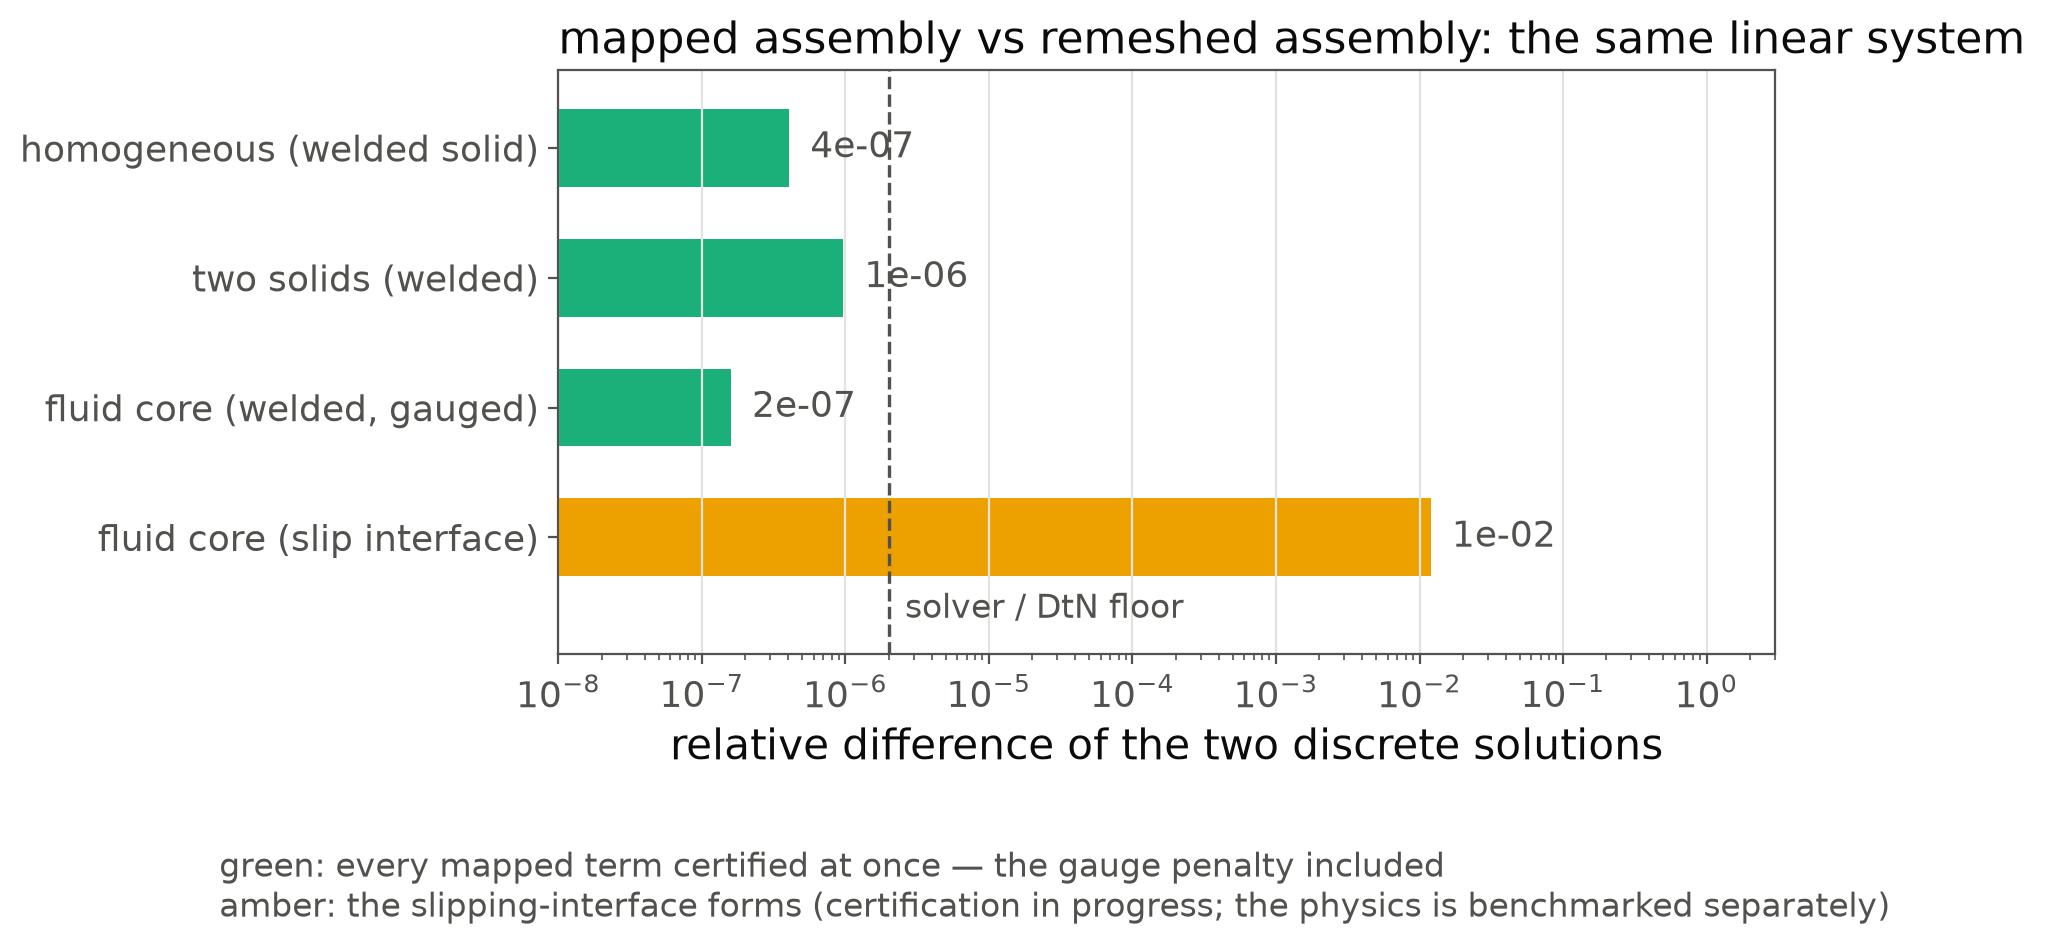
\includegraphics[width=0.75\textwidth]{talk_identity.png}
\caption{Talk figure: the identity per case. The slip value now comes
from the campaign's slip identity log (2 Oct; the script falls back to
the measured constant where no log exists).}
\end{figure}

\subsection{Leg C: an aspherical reference body (\code{aspherical\_reference})}

\textbf{Test.} The mesh is built by \code{meshes/aspherical\_body.py}:
a gmsh mesh of the ball whose nodes are moved by the radial stretch
\begin{equation}
  D(\vx) = (r+h)\,\rhat,\qquad
  h = \begin{cases} \eps\, r\, s(\theta,\varphi), & r\le 1,\\
                    \eps\, s\, q^2,\ q=\dfrac{1+B-r}{B}, & 1\le r\le 1+B,\end{cases}
  \label{eq:stretch}
\end{equation}
with $s = P_2(\cos\theta)+\beta\sin^2\theta\cos2\varphi$, $\beta=0.5$ and $B=0.2$, which is the identity on the DtN sphere. The
mesh is the reference body, and $\xi = D^{-1}$ maps it onto the unit
ball. The inverse is exact pointwise (linear inside, a cancellation-stable
quadratic root in the buffer), and $F=[F_D(\xi(\vy))]^{-1}$, so the run is
in exact-$F$ mode. Here the map is \emph{not} the identity on the surface:
the load is the physical harmonic pulled back with its Nanson area factor
$|J F^{-T}\vn|$. The solution is compared as fields with the pyslfp radial
solutions composed through $\xi$: the relative $L^2$ errors of $\vu$ over
the body and of the Eulerian potential $\phi_1=\zeta_1-\vb\cdot\vu$ for
$l=0,2,3,4$ ($l=1$ is skipped). The model is a single solid layer
(\code{homogeneous}), the gauge-free regime.

\textbf{Measured.} On the stock mesh ($\eps=0.05$), $\|\delta\vu\|$ is
$2.1$--$3.7\times10^{-2}$ and $\|\delta\phi\|$ $1.4\times10^{-3}$--$2.1\times10^{-2}$,
comparable to the spherical campaign at similar resolution. The README
claims the errors are independent of the shape amplitude ($\eps=0.05$ and
$0.02$ identical), but the stored ``$\eps=0.02$'' run was in fact the
$\eps=0.05$ case\review{r:aspherical}. A genuine sweep, made for this note
on meshes with the same gmsh connectivity at $\eps=0,0.02,0.05,0.08$
($\eps=0.1$ folds elements), confirms the claim
(Figure~\ref{fig:aspherical}): at fixed degree the errors vary by at most
4\,\% of themselves across the sweep, e.g.\ $\delta u_2 = 2.40, 2.43, 2.48,
2.49\times10^{-2}$. With elements halved ($\eps=0.05$) the errors drop
by 1.3--3.4 times.

One caveat for the interpretation: the aspherical mesh is the image under
$D$ of a spherical mesh, and $\xi=D^{-1}$ maps it back. Up to the
interpolation error of $D$ on the order-2 geometry, the pulled-back
discrete problem is therefore the spherical problem on the original
connectivity. Amplitude independence is to be expected; the test confirms
that the exact-$F$ volume and Nanson machinery reproduces this, with a
surface map that is not the identity. It is not an independent-mesh test
in the sense of a mesh generated on the aspherical body directly.

\begin{figure}[H]
\centering
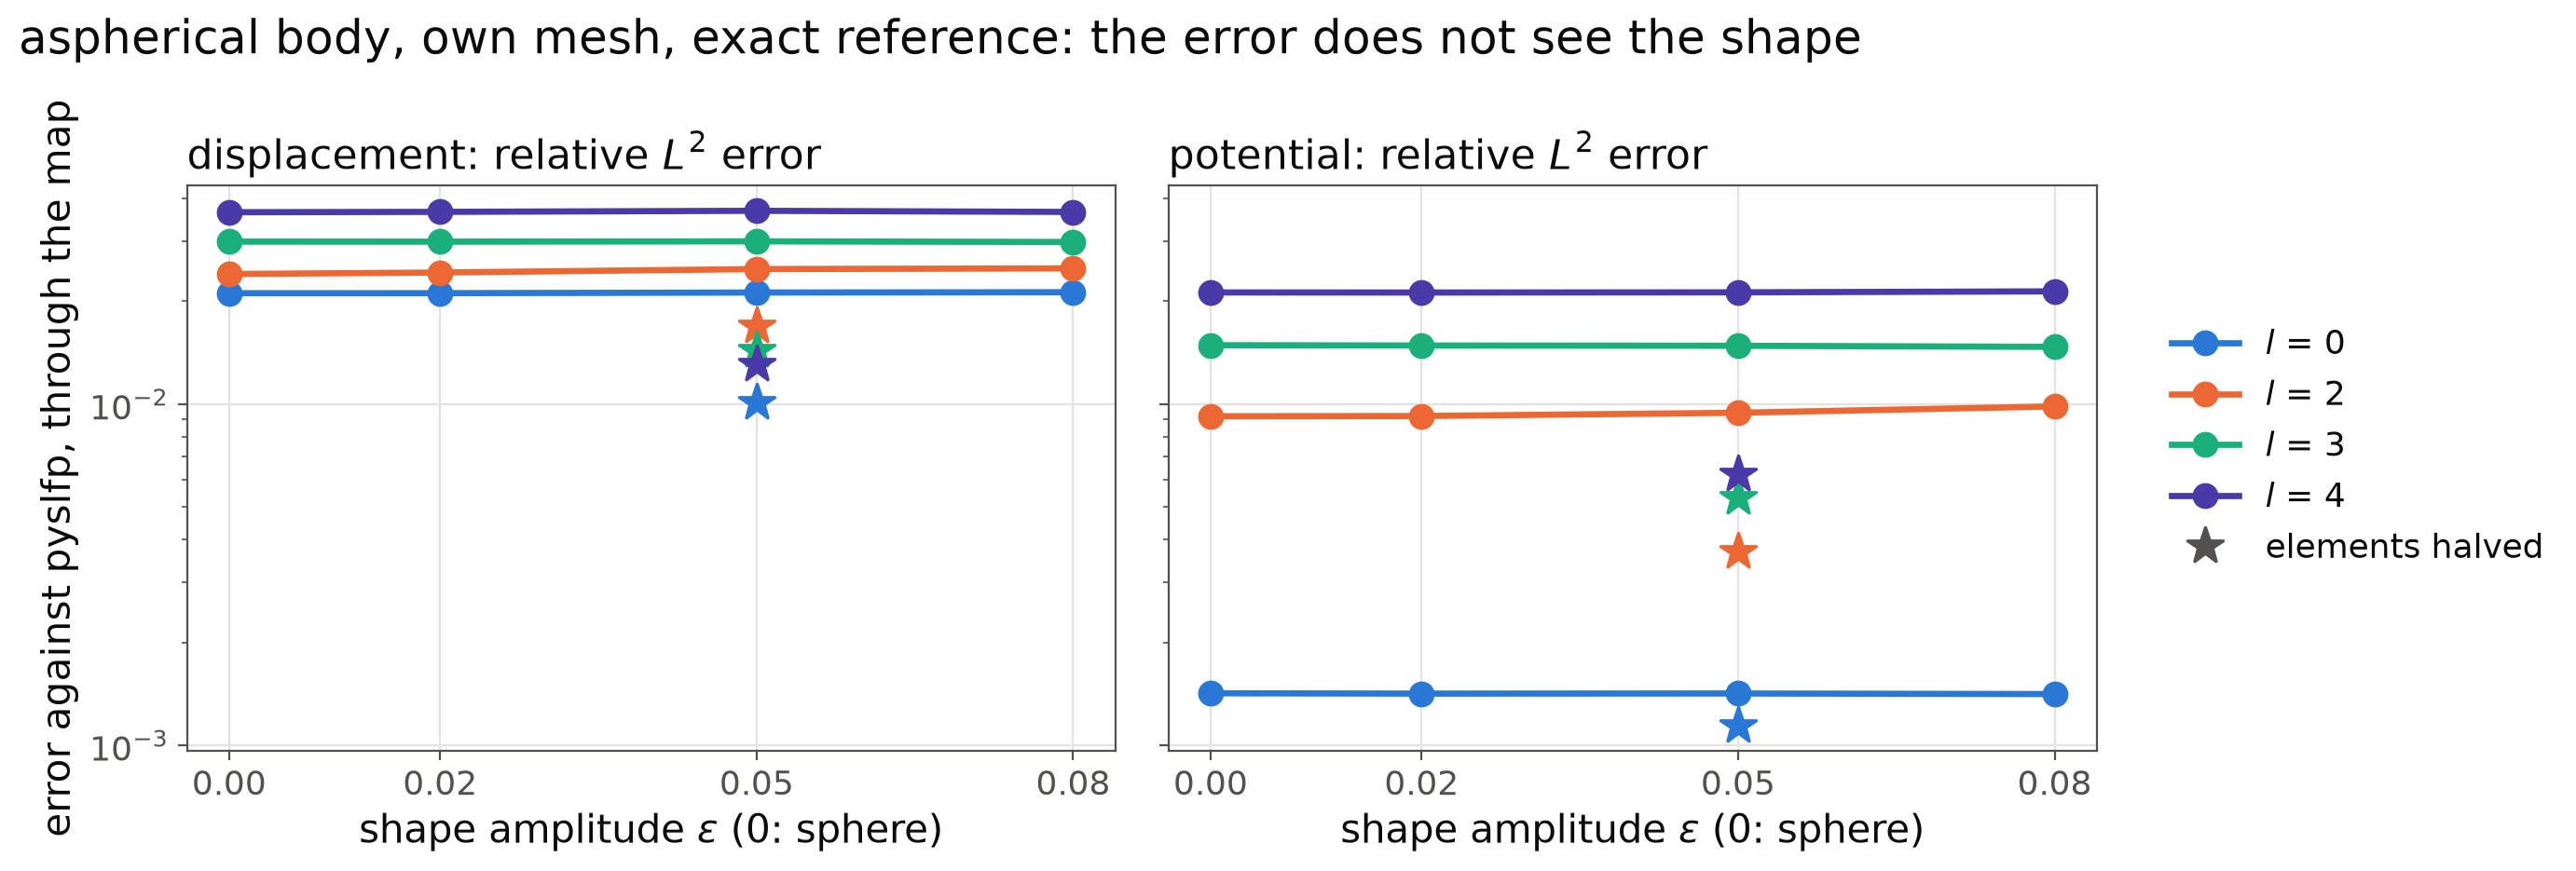
\includegraphics[width=\textwidth]{talk_aspherical.png}
\caption{Aspherical body: relative field errors against pyslfp through
the map, against the shape amplitude (0 is the spherical mesh with the
same connectivity), by degree. Stars: elements halved. Rebuilt from the
new amplitude sweep.}
\label{fig:aspherical}
\end{figure}

%=============================================================================
\section{The perturbation family}
\label{sec:pert}
%=============================================================================

\subsection{What is tested, and the aim}

This family checks \emph{derivatives} of the response with respect to the
model, which is the first step towards adjoint and topography kernels.
Its first member needs no new theory: the radius $r_k$ of one interior
interface is shifted by $\eps$. Every member of the family is still
spherical, so pyslfp solves it exactly. The 3-D solver describes each
member from \emph{one fixed mesh}, through the piecewise-linear radial map
\begin{equation}
  \xi(\vx) = f(r)\,\rhat,\qquad f \text{ affine on each } [b_j,b_{j+1}],\quad
  f(b_j) = b_j + \eps\,\delta_{jk},
  \label{eq:shift}
\end{equation}
\begin{equation*}
  F = f'(r)\,\rhat\rhat^T + \frac{f}{r}\bigl(I-\rhat\rhat^T\bigr),
\end{equation*}
which moves interface $k$ and fixes the centre, the other interfaces and
the surface. $F$ is discontinuous across the interfaces, which the
per-region forms allow. The comparison is between central differences,
\begin{equation}
  D_{3\text{D}} = \frac{R_{3\text{D}}(+\eps)-R_{3\text{D}}(-\eps)}{2\eps}
  \quad\text{vs}\quad
  D_{1\text{D}} = \frac{R_{\text{pyslfp}}(+\eps)-R_{\text{pyslfp}}(-\eps)}{2\eps},
  \label{eq:fd}
\end{equation}
for each load Love number $R$. Both are $\partial R/\partial r_k+O(\eps^2)$.
Because the mesh is fixed, the discretisation bias $R_{3\text{D}}-R$ is a
smooth function of $\eps$ and largely cancels in $D_{3\text{D}}$. The
comparison therefore tests the \emph{derivative}, through the mapped
assembly, at an accuracy better than that of $R_{3\text{D}}$ itself.
Note that $D_{1\text{D}}$ is a finite difference of pyslfp solves, not an
analytic perturbation-theory kernel\review{r:derivlabel}.

\subsection{Assumptions and implementation details}

\begin{itemize}[leftmargin=*]
\item The perturbed model is built by moving the interface in the SI
  model (\code{models.SHIFTABLE}) and is re-scaled with the same outer
  radius. Its mass differs from the base model's at $O(\eps)$,
  $\mathrm{d}M/\mathrm{d}r_k = 4\pi r_k^2[\rho]$. The driver therefore
  takes the mass, the surface gravity and the interface gravities from
  the perturbed model's exact profiles (\code{RadialProfiles::EnclosedMass}),
  not from mesh integrals of the base fields. The Love-number
  normalisation \eqref{eq:loadlove} depends on this: a $2\%$ error in $g$
  at $\eps=0.02$ would otherwise swamp the derivative.
\item Shift runs use the interpolated $F$. The exact map's slope jumps at
  the moving interface, and on curved facets the quadrature points of
  the one-sided interface kernels lie $O(h^2)$ inside the analytic
  radius, so they picked up the fluid-side slope. That was the whole of
  the earlier outward-shift pathology of slip\_broken. The interpolation
  perturbs the model by $O(h^p)$ consistently at both signs, which cancels
  in \eqref{eq:fd}.
\item Every augmented-Lagrangian sweep runs at full tolerance in shift
  runs, so that the endpoints are reproducible.
\item Comparisons: $h'$ at every degree, $l'$ and $k'$ from degree 2,
  degree 1 skipped, near-zero derivatives skipped.
\end{itemize}

\subsection{Results}

Campaign of 1 Oct: $\eps=\pm0.02$, $h=0.3$, order 2, degrees $0$--$3$.
\begin{center}
\small
\begin{tabular}{@{}llP{10cm}@{}}
\toprule
model & method & $|D_{3\text{D}}-D_{1\text{D}}|/|D_{1\text{D}}|$ \\
\midrule
\code{fluid\_core} & referential & $h'_0$ 0.8\,\%, $h'_2$ 6.5\,\%, $l'_2$ 12\,\%, $k'_2$ 1.8\,\%, $h'_3$ 1.9\,\%, $l'_3$ 15\,\%, $k'_3$ 0.9\,\% \\
\code{fluid\_core} & slip\_broken & $h'_0$ 0.8\,\%, $h'_2$ 25\,\%, $l'_2$ 2.8\,\%, $k'_2$ 39\,\%, $h'_3$ 5.1\,\%, $l'_3$ 20\,\%, $k'_3$ 11\,\% \\
\code{two\_solid} & referential & $h'_0$ 2.9\,\%, $h'_2$ 8.3\,\%, $l'_2$ 5.1\,\%, $k'_2$ 12\,\%, $h'_3$ 17\,\%, $l'_3$ 5.1\,\%, $k'_3$ 11\,\% \\
\bottomrule
\end{tabular}
\end{center}
The degree-0 derivative agrees to 0.8\,\% for both methods on
\code{fluid\_core}, and the referential method's $k'$ derivatives agree to
1--2\,\%. The degree-2 and $l'$ entries are worse, and slip\_broken's
degree-2 derivatives are off by 25--40\,\%, which is more than the
README's ``few-percent'' summary suggests\review{r:pertslip}. The absolute
agreement at each $\eps$ (left panels) is flat across the ladder: the
mapped solves track the perturbed models as well as the unmapped solve
tracks the base model. Its degree-2 value, about 17\,\% and set by
$l'_2$, is the same for every $\eps$ and both methods. The README
attributes it to the $O(N^2)$ mismatch of the compressible methods on
this non-neutral core. On \code{two\_solid} the derivatives are small (the
interface lies deep, with modest jumps), and relative discrepancies of
5--17\,\% are within an order of magnitude of the error of the numbers
themselves. A ladder in $\eps$ (0.01, 0.02), as the server profile has,
would separate the $O(\eps^2)$ remainder from discretisation.

\begin{figure}[H]
\centering
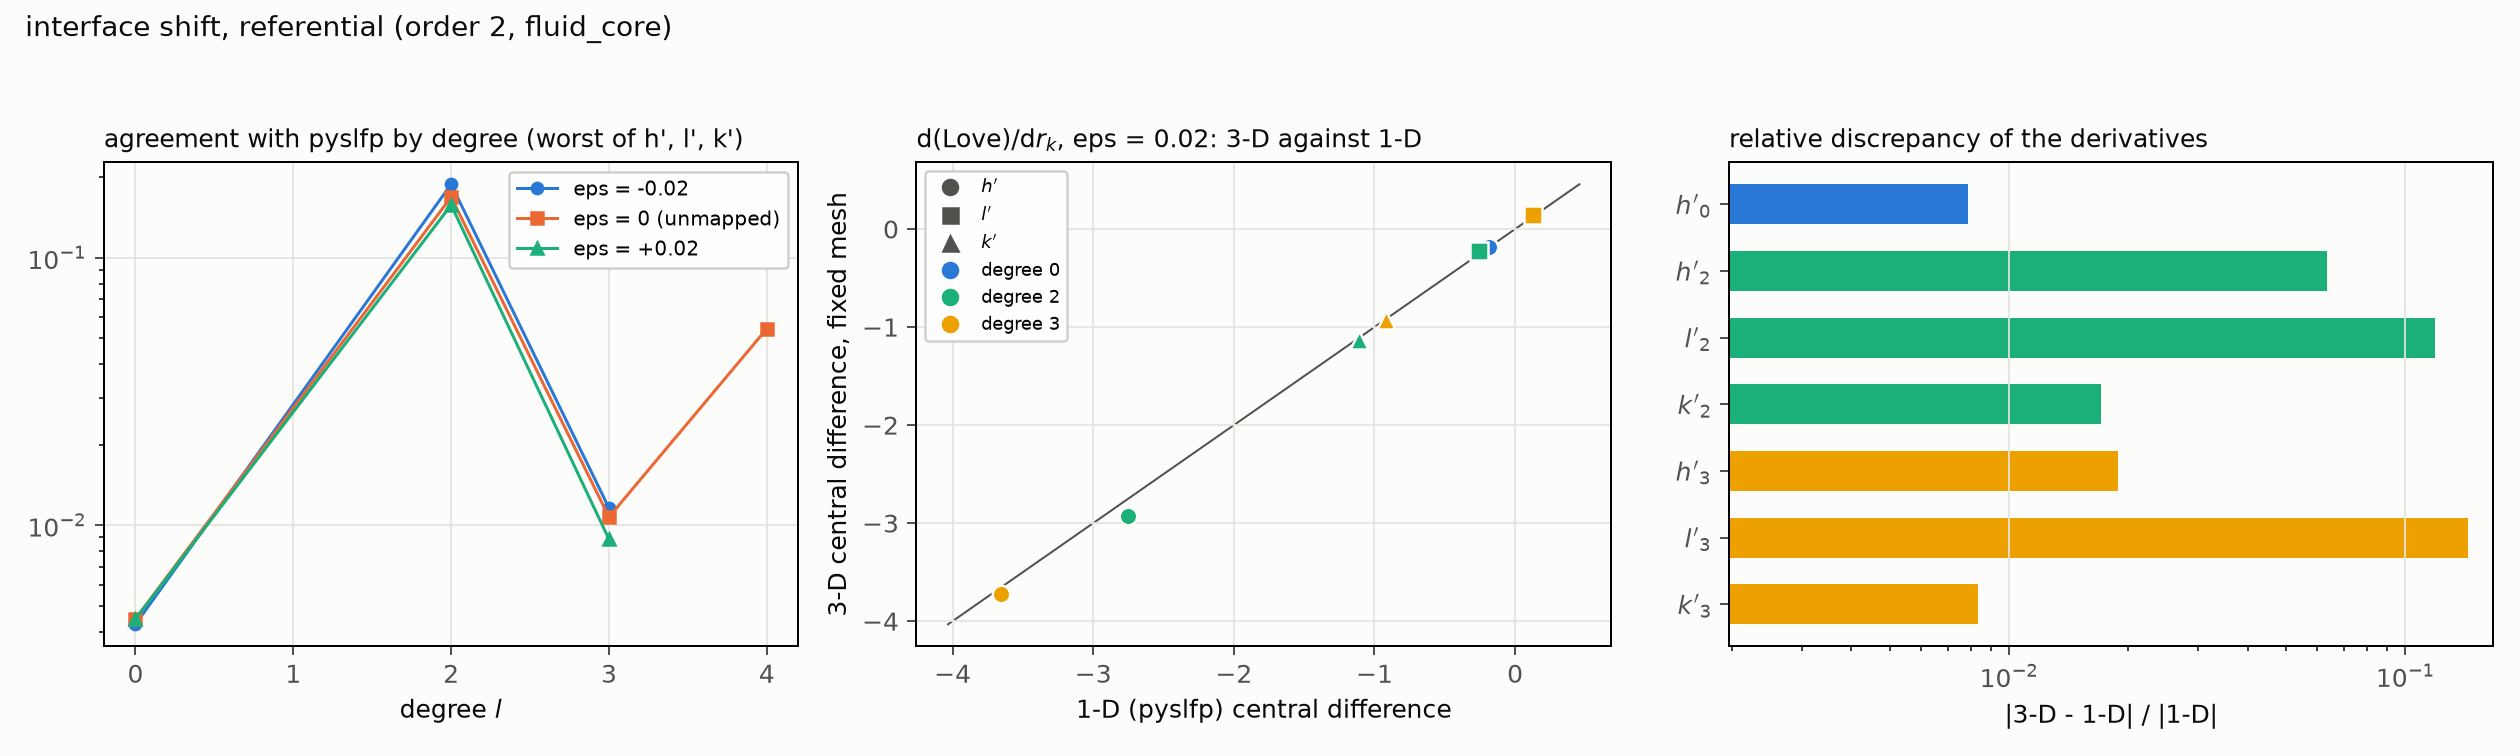
\includegraphics[width=\textwidth]{pert_fc_referential.png}\\[1ex]
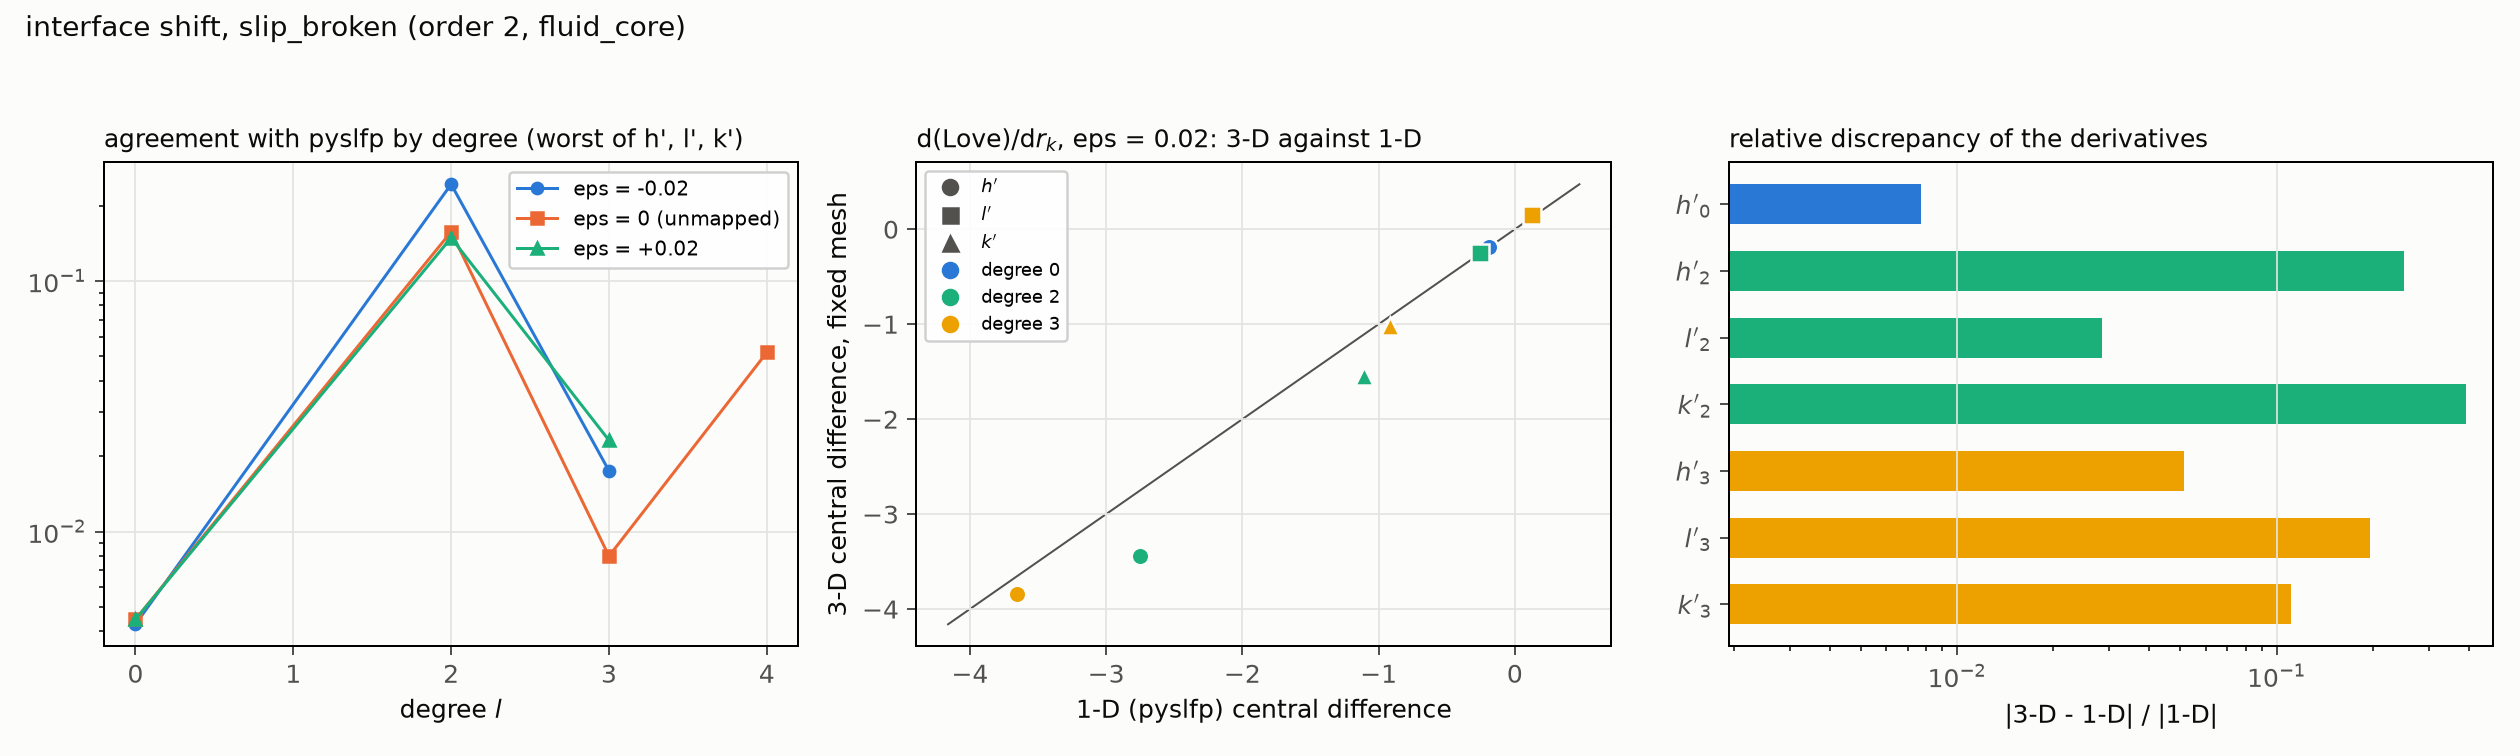
\includegraphics[width=\textwidth]{pert_fc_slip_broken.png}\\[1ex]
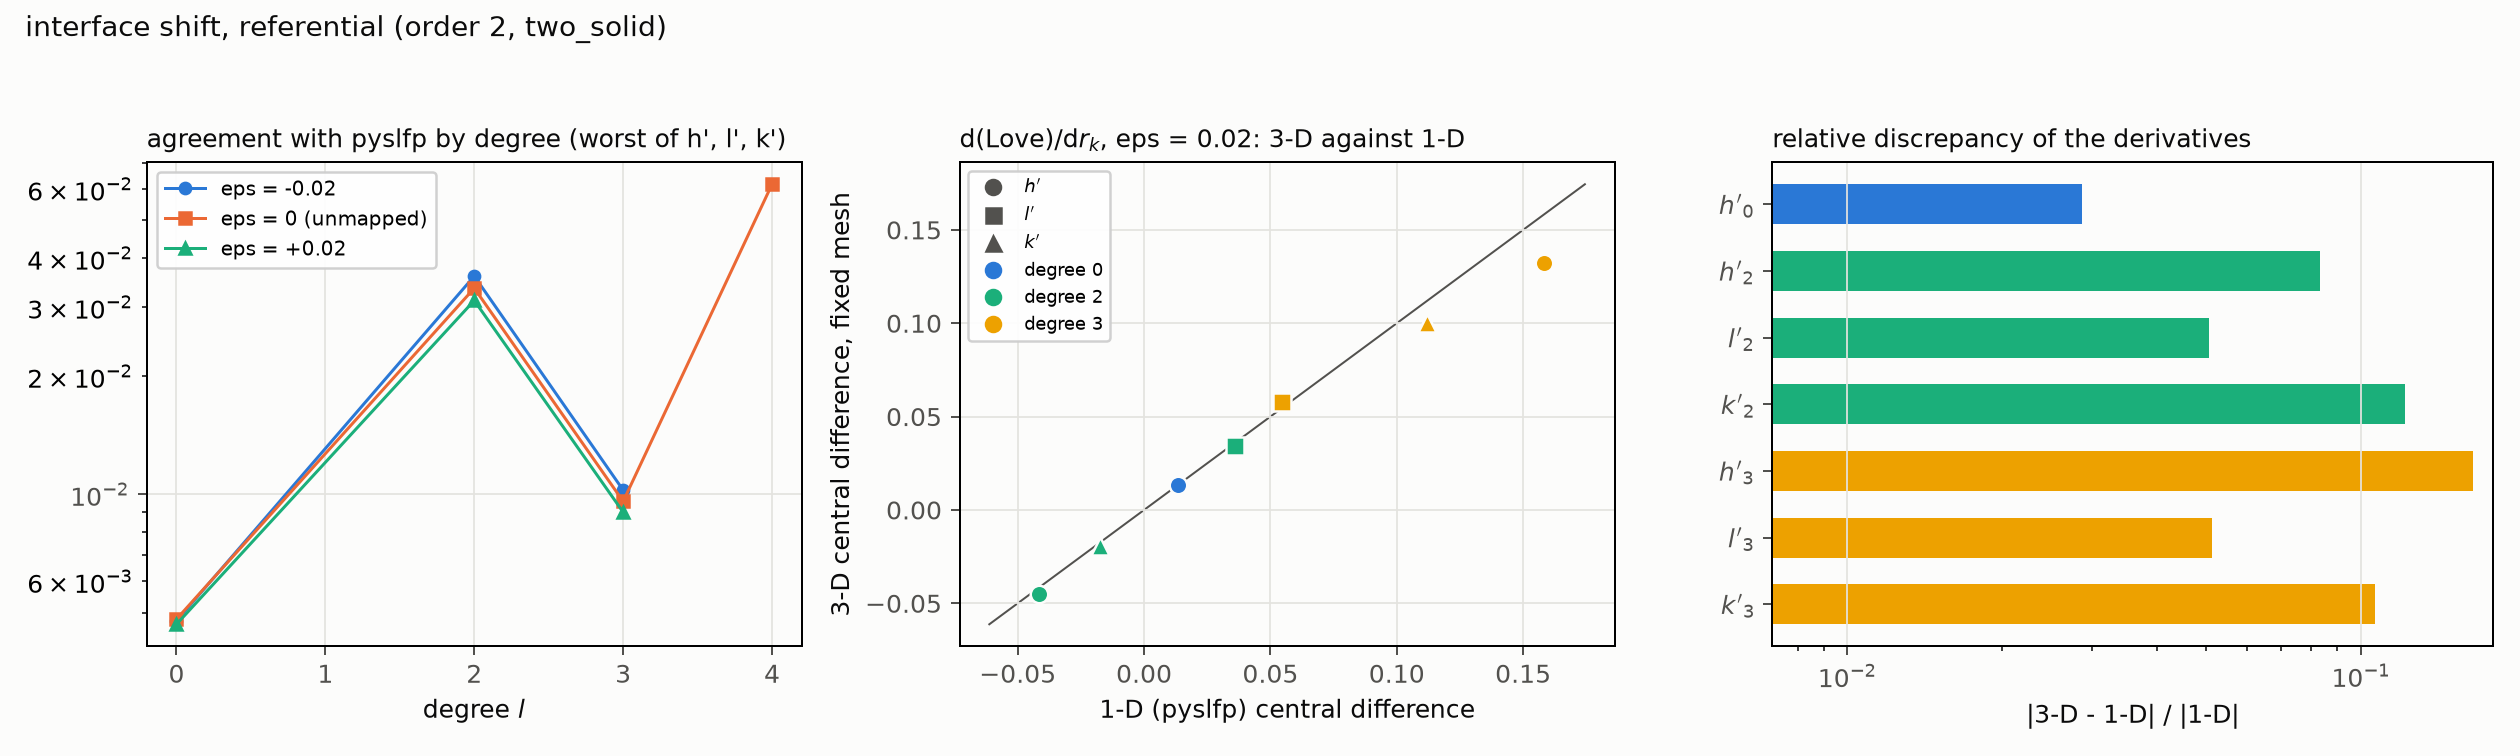
\includegraphics[width=\textwidth]{pert_ts_referential.png}
\caption{Interface-shift check, redrawn: absolute agreement with pyslfp by
degree and shift (left); the 3-D central difference against the 1-D one
(middle; Love number by marker, degree by colour); and the relative
discrepancy of each derivative (right), which the identity plot cannot
resolve for the small derivatives. Top: \code{fluid\_core} referential;
middle: \code{fluid\_core} slip\_broken; bottom: \code{two\_solid}
referential.}
\end{figure}

\begin{figure}[H]
\centering
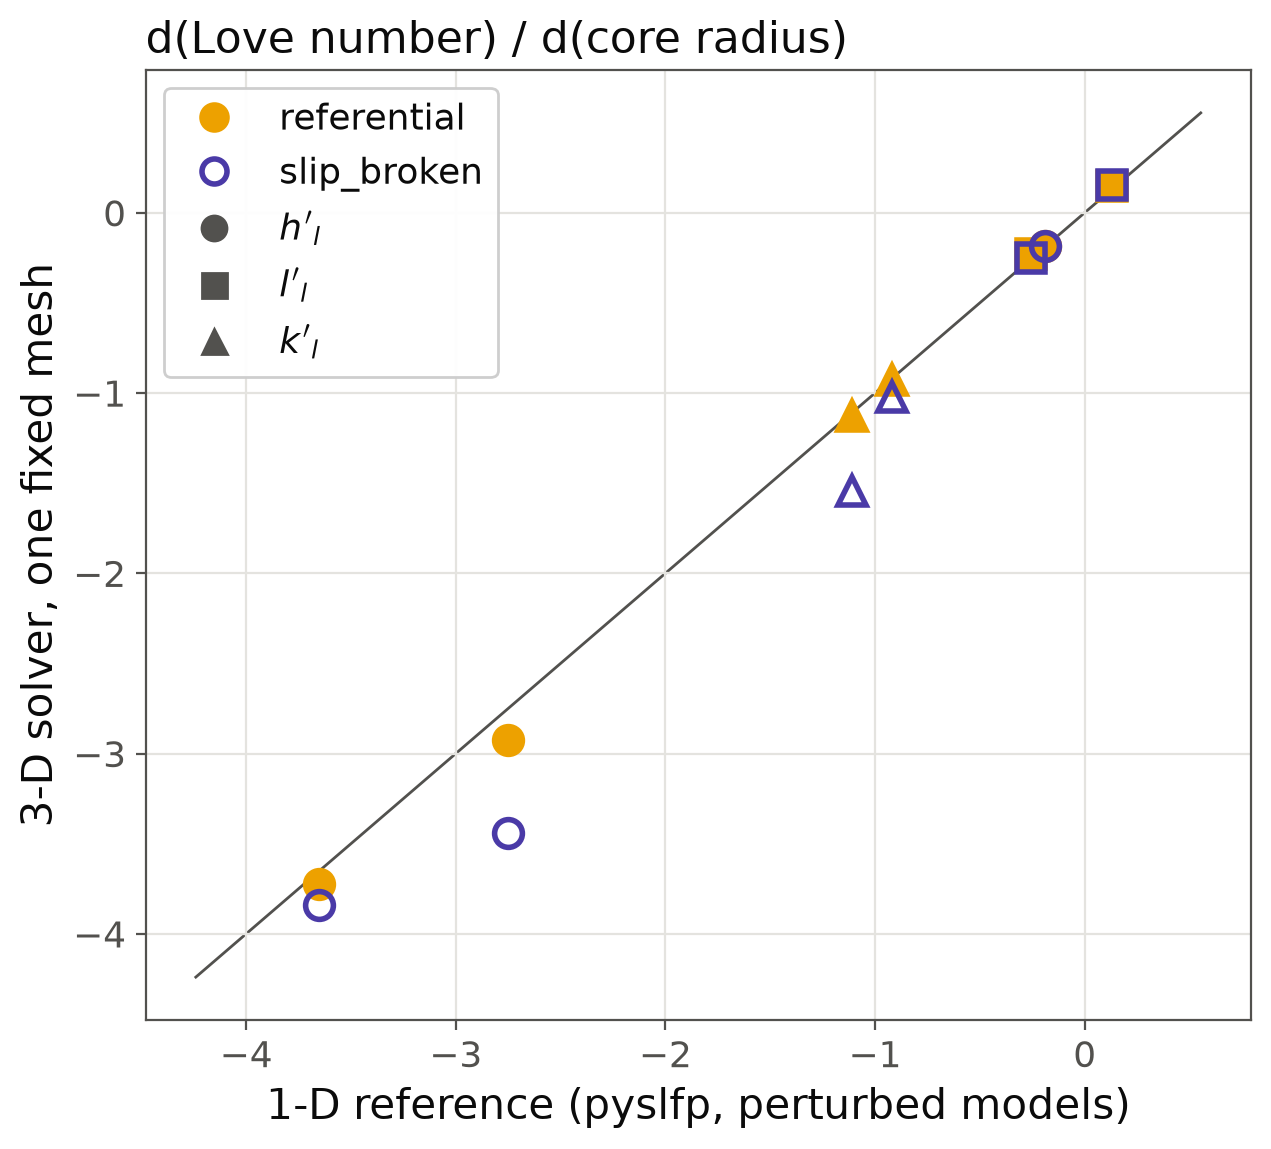
\includegraphics[width=0.5\textwidth]{talk_derivative.png}
\caption{Talk figure: both methods on one identity plot, from the
1 Oct runs. The earlier version read the 30 Sep slip\_broken shift runs,
made before the outward-shift fix.}
\end{figure}

%=============================================================================
\section{The viscoelastic family}
\label{sec:visco}
%=============================================================================

The family tests \code{ViscoelasticOperator}, its integrators and the
rheologies, in four sub-families of \code{benchmarks/viscoelastic/}:
\begin{center}
\small
\begin{tabular}{@{}lP{8.2cm}P{4.2cm}@{}}
\toprule
sub-family & what is tested & reference \\
\midrule
\code{box/} (\S\ref{sec:box}) & non-gravitating, solid-only problems on
rectangular meshes, 2-D and 3-D: homogeneous bodies (the integrators
alone), laterally uniform columns, Fourier-mode loading of layered slabs;
general load histories, multi-branch rheologies, viscosity contrasts to
$10^8$ & exact (closed-form modes and convolutions; AAA and Talbot) \\
\code{sphere/} (\S\ref{sec:sphere}) & non-gravitating layered balls and
discs under surface loads of degree $l$; smooth lateral viscosity
contrasts for the integrators & exact for radial models (Euler-type radial
system, AAA, Talbot); a much smaller step for lateral ones \\
\code{stepping/} (\S\ref{sec:survey}) & the stepper survey on the beam of
\code{examples/viscoelastic\_schemes} & RK4 at a small step \\
\code{love/} (\S\ref{sec:laplace}) & Maxwell load Love-number histories of
gravitating spherical models & pyslfp, correspondence principle,
Gaver--Stehfest \\
\bottomrule
\end{tabular}
\end{center}
The box and sphere sub-families separate the time integration and the
viscoelastic discretisation from gravity and fluids (the box from
spherical geometry as well), which the quasi-static elastic families
test on their own. Its references are exact
to about $10^{-10}$, so any mismatch is the code's. That is what lets it
cover many situations cheaply: every forcing against every scheme, step
ladders, mesh ladders, and contrasts of eight decades. The Love-number
histories remain the integrated test of the self-gravitating machinery.

\subsection{The time integrators}
\label{sec:steppers}

This subsection summarises how each integrator tested below works: what it
computes per step, what it costs, and where its order and stability come
from. The implementation is \code{ViscoelasticOperator}
(\code{src/viscoelastic.cpp}); \code{doc/viscoelasticity.md} has the
design notes.

\paragraph{The semi-discrete system.}
The state is the set of internal variables $m_k$, one per Prony branch,
held at the nodes of an L2 space. The displacement is not a state
variable. It is slaved to $m$ through one quasi-static solve with the
\emph{unrelaxed} stiffness $K_U$:
\begin{equation}
  K_U u = f(t) + \sum_k B_k^{T} C_k m_k,\qquad d = D u,\qquad
  \dot m_k = \frac{d - m_k}{\tau_k},
  \label{eq:ve-semidiscrete}
\end{equation}
where $B$ is the strain coupling, $D$ the strain map (Galerkin projection),
$C_k$ the branch modulus applied pointwise, and $d$ the (deviatoric)
strain at the nodes. Every evaluation of $d$ costs one elastic solve, which
is why cost is counted in solves. Write $h_k=\Delta t/\tau_k$, a nodal field
because $\tau_k$ varies in space. For a linear body,
\eqref{eq:ve-semidiscrete} is a linear ODE $\dot m=-Lm+g(t)$. In a
homogeneous body its decay rates lie between $\mu_\infty/(\mu_U\tau)$
(stress control: the creep or retardation rate, zero for a Maxwell body)
and $1/\tau$ (strain control: relaxation). In general the stiffest rate is
of order $1/\tau_{\min}$, and this is what bounds explicit steps.

\paragraph{Eliminating the end state (effective modulus).}
The implicit and trapezoid schemes need $d^{n+1}$, which depends on
$m^{n+1}$. Every such update has the form
$m_k^{n+1}=a_k + b_k\,d^{n+1}$ with nodal $a_k$ and $b_k$. Substituting it
into \eqref{eq:ve-semidiscrete} at $t_{n+1}$ and using
$B^{T}C_kD=K(C_k)$ (exact when the internal order resolves $\eps(u)$)
removes $m^{n+1}$ and leaves one elastic solve with an \emph{effective
modulus}:
\begin{equation}
  K\Bigl(C_\infty+\sum_k\beta_kC_k\Bigr)\,u^{n+1}
  = f(t_{n+1}) + \sum_k B_k^{T}C_k\,a_k,
  \qquad \beta_k = 1-b_k .
  \label{eq:ve-effective}
\end{equation}
$\beta_k\in(0,1]$ is a nodal weight. It is 1 for $h\to0$ (the unrelaxed
operator) and tends to 0 for $h\to\infty$, where the branch has relaxed
and the operator is the long-term one, $K(C_\infty)$. A change of
$\Delta t$ changes $\beta$, so the operator must be reassembled and,
eventually, the preconditioner rebuilt. With a fixed step the operator is
assembled once.

\paragraph{Explicit Runge--Kutta (RK4).}
\code{Mult} evaluates the rate: one solve with $K_U$ at the stage time,
then $(d-m_k)/\tau_k$ pointwise. Any explicit MFEM solver can drive it. The
tested one is classical RK4: four solves per step and fourth order. The
operator never changes. Its stability interval on the negative real axis
is about $[-2.785,0]$, so $\Delta t\lesssim2.8\,\tau_{\min}$ whatever the
accuracy needed. That is cheap when nothing is stiff and hopeless when
$\tau_{\max}/\tau_{\min}$ is large.

\paragraph{Exponential Euler (ETD1).}
Solve with $K_U$ at $t_n$ for $d^n$, then relax exactly with the strain
frozen over the step:
\begin{equation}
  m_k^{n+1} = e^{-h_k}m_k^{n} + \bigl(1-e^{-h_k}\bigr)\,d^{n}.
\end{equation}
This is the exact solution of $\dot m=(d-m)/\tau$ for constant $d$. The
local error is $O(\Delta t^2\dot d)$, so the scheme is first order. It
takes one solve per step, always with $K_U$ (no reassembly), and has no
step restriction. Under creep ($d$ growing) it lags systematically. It is
also the embedded companion of the adaptive scheme.

\paragraph{Exponential trapezoid (ExpTrap).}
By variation of constants,
\begin{equation}
  m_k(t_{n+1}) = e^{-h_k}m_k^{n}
   + \frac{1}{\tau_k}\int_0^{\Delta t}e^{-(\Delta t-s)/\tau_k}\,d(t_n+s)\,\mathrm{d}s .
\end{equation}
ExpTrap replaces $d$ by its linear interpolant between $d^n$ and $d^{n+1}$
and integrates exactly:
\begin{equation}
  m_k^{n+1} = e^{-h}m_k^{n} + \alpha\,d^{n} + \beta\,d^{n+1},\qquad
  \alpha = \frac{1-e^{-h}}{h}-e^{-h},\quad
  \beta = 1-\frac{1-e^{-h}}{h}
\end{equation}
(series for small $h$). In the form of \eqref{eq:ve-effective},
$a_k=e^{-h}m_k^n+\alpha d^n$ and the weight is
$\beta_k=1-\beta=(1-e^{-h})/h$. It takes one solve per step: $d^n$ is
reused from the previous step's end, which is cached, so only the first
step pays for an extra unrelaxed solve. The load is evaluated at
$t_{n+1}$. Properties:
\begin{itemize}[leftmargin=*]
\item second order, and \emph{exact} whenever the strain is linear in
  time over the step (Maxwell creep under constant stress at any
  $\Delta t$);
\item for $h\to0$, $\alpha,\beta\to h/2$: the ordinary trapezoid rule;
\item for $h\to\infty$, $\alpha\to0$ and $\beta\to1$: $m^{n+1}=d^{n+1}$
  with the long-term operator, which is exactly the relaxed equilibrium.
  The decay factor $e^{-h}$ is exact, so there is no step restriction and
  no oscillation (Crank--Nicolson, by contrast, has amplification
  $\to-1$ there and is deliberately absent);
\item the error is controlled by how far $d$ is from linear over a step,
  i.e.\ by $\Delta t^2\ddot d$. A fast or kinked load costs accuracy, not
  stability.
\end{itemize}

\paragraph{Backward Euler (BE).}
Through MFEM's \code{BackwardEulerSolver}: \code{ImplicitSolve} returns
the rate $k=(m^{n+1}-m^n)/\Delta t$ with
\begin{equation}
  m_k^{n+1} = \frac{m_k^{n} + h_k\,d^{n+1}}{1+h_k},\qquad
  \beta_k = \frac{1}{1+h_k},\quad a_k=\frac{m_k^n}{1+h_k},
\end{equation}
and the load is evaluated at $t_{n+1}$. It takes one solve per step and is
first order and L-stable (amplification $1/(1+h)\to0$). For $h\gg1$ it
returns the relaxed equilibrium like ExpTrap, but its error at moderate
$h$ is $O(\Delta t)$.

\paragraph{SDIRK23 (MFEM \code{SDIRK23Solver(2)}).}
This is a two-stage singly diagonally implicit RK method with
$\gamma=1-1/\sqrt2\approx0.293$:
\begin{equation}
\begin{aligned}
  k_1 &= F\bigl(t_n+\gamma\Delta t,\; m^n+\gamma\Delta t\,k_1\bigr),\\
  k_2 &= F\bigl(t_n+(1-\gamma)\Delta t,\; m^n+(1-2\gamma)\Delta t\,k_1+\gamma\Delta t\,k_2\bigr),\\
  m^{n+1} &= m^n + \tfrac{\Delta t}{2}(k_1+k_2),
\end{aligned}
\qquad
\begin{array}{c|cc}
  \gamma & \gamma & \\
  1-\gamma & 1-2\gamma & \gamma\\ \hline
  & \tfrac12 & \tfrac12
\end{array}
\end{equation}
Each stage is a backward-Euler solve of step $\gamma\Delta t$ (weights
$1/(1+\gamma h)$). Both stages share one effective operator, so it costs
two solves and one assembly per step size. It is second order
($b^{T}c=\tfrac12$; this $\gamma$ is not the third-order one) and
L-stable: $R(\infty)=1-b^{T}A^{-1}\mathbf 1=1-(4\gamma-1)/(2\gamma^2)=0$
exactly for this $\gamma$. It has stage order 1, and the stage loads are
taken at $t_n+\gamma\Delta t$ and $t_n+(1-\gamma)\Delta t$. MFEM's default
\code{SDIRK23Solver()} is the third-order, A- but not L-stable variant;
the drivers use the L-stable one. Note that the displacement left by the
second stage belongs to the stage state, not to $m^{n+1}$, so an
observation between steps costs an extra unrelaxed solve (and a switch
of operator). BE and ExpTrap leave a consistent displacement.

\paragraph{Adaptive exponential trapezoid.}
Each trial step is an ExpTrap step. Its ETD1 companion $\hat m$ (nodal
work only, no solve) gives a free first-order error estimate
\begin{equation}
  \text{err} = \Bigl[\tfrac1N\sum_j\Bigl(\frac{m_j^{n+1}-\hat m_j}
   {\text{atol}+\text{rtol}\max(|m_j^n|,|m_j^{n+1}|)}\Bigr)^2\Bigr]^{1/2},
  \qquad
  \Delta t\leftarrow\Delta t\cdot\min\bigl(4,\max(0.2,\,0.9\,\text{err}^{-1/2})\bigr).
\end{equation}
A step with err $>1$ is rejected and retried. The exponent $1/2$ matches
the $O(\Delta t^2)$ local error of the first-order companion. Because the
estimate belongs to ETD1, it is conservative for the propagated
second-order solution, by a factor of order $\tau/\Delta t$. There is no
stability limit, so adaptivity is purely about accuracy: small steps
where the load or $\tau$ changes quickly, long strides across quiet
periods. The price is that every accepted step has a new $\Delta t$,
hence new weights and a reassembly (the preconditioner is reused while
the iteration count stays within a factor 2 of its count at setup), and
every rejected step costs a solve.

\paragraph{State-dependent relaxation times.}
With a power law, $\tau_k$ depends on the stress. ExpTrap and the implicit
stages then run a predictor--corrector. The first pass uses the times of
the start state. The times are then re-evaluated at the midpoint state
(ExpTrap) or the end state (BE, SDIRK stages) and the step is repeated,
by default once. Each pass is an extra solve with a different effective
operator. ETD1 and the explicit schemes simply use the current times.

\begin{table}[H]
\centering
\small
\begin{tabular}{@{}lccccl@{}}
\toprule
scheme & order & solves/step & operator & stability & exact when \\
\midrule
RK4 & 4 & 4 & $K_U$ & $\Delta t\lesssim2.8\,\tau_{\min}$ & --- \\
ETD1 & 1 & 1 & $K_U$ & unconditional & $d$ constant over the step \\
ExpTrap & 2 & 1 & effective & unconditional & $d$ linear over the step \\
BE & 1 & 1 & effective & L-stable & --- \\
SDIRK23 & 2 & 2 & effective (one per $\Delta t$) & L-stable & --- \\
Adaptive & 2 (est.\ 1) & 1 per trial & effective, new per step & unconditional & as ExpTrap \\
\bottomrule
\end{tabular}
\caption{The tested integrators. ``Operator'' is the stiffness that the
step's solves use; ``effective'' is \eqref{eq:ve-effective}, assembled
once per step size.}
\label{tab:steppers}
\end{table}

\subsection{Box benchmarks: problems and exact references}
\label{sec:box}

\paragraph{What is tested, and the aim.}
The question is whether \code{ViscoelasticOperator} and its integrators
are right, and how accurate and costly they are, over a wide range of
situations: forcings with jumps, kinks and periodic transients, rheologies
with one to four relaxation times, viscosity contrasts up to $10^8$, and
spatially structured responses in 2-D and 3-D. Gravity, fluids and
spherical geometry are left out on purpose, since the elastic families
test them. What remains has exact references, so every error is measured
against the truth, not against another numerical method.

\paragraph{Geometry and loads.}
The body is the box $[0,L_x]\times[0,H]$ (2-D) or
$[0,L_x]\times[0,L_y]\times[0,H]$ (3-D), with $z$ the last coordinate and
horizontal layers stacked from $z=0$. Meshes are Cartesian quadrilaterals
or hexahedra from \code{Mesh::MakeCartesian*}, and a \emph{slab} is made
periodic sideways (\code{Mesh::MakePeriodic}). Every load is an amplitude
times a history $S(t)$:
\begin{itemize}[leftmargin=*]
\item \code{uniaxial\_stress} (box, \code{LinearQuasiStaticTractionProblem}):
  tractions $\pm S(t)\,e_x$ on $x=L_x$ and $x=0$. Uniaxial stress
  $\sigma=S\,e_x\otimes e_x$ is a homogeneous state.
\item \code{uniaxial\_strain} (box, \code{LinearQuasiStaticClampedProblem}):
  the whole boundary prescribed, $u=S(t)\,x\,e_x$: time-dependent
  Dirichlet data, again homogeneous.
\item \code{surface} (slab, clamped base): the normal pressure
  $p(x,t)=S(t)\cos k_xx\cos k_yy$ on $z=H$, with $k_i=2\pi n_i/L_i$. Mode
  $n=0$ is a uniform pressure (the laterally uniform \emph{column}).
\end{itemize}
In the homogeneous problems the finite elements are exact in space at any
order, so every error is the integrator's. The column is exact in space
when layer interfaces lie on element faces and the moduli are constant
in each layer. The Fourier slab has genuine spatial error.

The 2-D problems are the library's two-dimensional continuum
($\lambda=\kappa-\mu$, the 2-D deviator), not plane strain of a 3-D body.
The references use $\lambda=\kappa-2\mu/d$ with $d$ the space dimension,
so each convention is checked on its own terms.

\paragraph{Models.}
All are nondimensional, with $\kappa=5/3$ and shear moduli of order one.
Time is in units of the reference Maxwell time ($\tau=1$).
\begin{center}
\small
\begin{tabular}{@{}lP{11.6cm}@{}}
\toprule
model & definition (layers bottom-up; $H=1$) \\
\midrule
\code{maxwell} & $\mu_\infty=0$, one branch $(\mu,\tau)=(1,1)$ \\
\code{sls} & standard linear solid: $\mu_\infty=0.5$, one branch $(0.5,1)$ \\
\code{burgers} & $\mu_\infty=0$, branches $(0.6,1)$, $(0.4,0.05)$: two relaxation times \\
\code{prony\_wide} & $\mu_\infty=0.1$, four branches $0.225$ at $\tau=10^{-3},10^{-1},10,10^3$: six decades \\
\midrule
\code{maxwell\_slab} & one Maxwell layer: no elastic support, so a non-uniform load makes it \emph{flow} (a pole at $s=0$) \\
\code{lid} & Maxwell $[0,0.8]$, elastic lid $[0.8,1]$ \\
\code{channel} & Maxwell $[0,0.6]$, low-viscosity channel $[0.6,0.8]$ with $\tau=1/C$, elastic lid \\
\code{sls\_stack} & standard linear solids: $(\mu_\infty,\mu_1,\tau)=(0.5,0.5,1)$ below $0.6$, $(0.3,0.7,10)$ above \\
\code{burgers\_lid} & the Burgers mantle $[0,0.8]$ under an elastic lid \\
\code{prony\_lid} & $\mu_\infty=0.1$ and branches $0.3$ at $\tau=10^{-2},1,10^2$, $[0,0.8]$, under an elastic lid \\
\code{contrast} & Maxwell $\tau=1$ $[0,0.4]$, $\tau=1/C$ $[0.4,0.6]$, $\tau=C$ $[0.6,0.8]$, elastic lid: the contrast ladder \\
\code{gradient} & one Maxwell layer $[0,0.8]$ with $\tau$ geometric from $1/C$ at the base to $1$ at its top, elastic lid \\
\bottomrule
\end{tabular}
\end{center}
\emph{The mesh comes first.} Every layer interface is a multiple of
$0.2$, the cell size of the coarsest mesh of the ladders ($n_z=5$), so
every uniform mesh with $n_z$ a multiple of 5 has the material
discontinuities on element faces. The driver refuses a mesh that cuts a
layer, except for the deliberate misfit of the interface study
(\code{-no-conform}, \S\ref{sec:box-slab}).

Without gravity there is no isostatic restoring force. A Maxwell body
with nothing elastic in it therefore has no bounded response to a
non-uniform load (\code{maxwell\_slab} flows), while under a uniform load
it relaxes to its $\kappa$-response. Elastic lids or standard linear
solids give bounded responses.

\paragraph{Load histories.}
A history is a sum of \emph{pieces}, each
\begin{equation}
  w(s) = c_0 + c_1 s + a\cos\omega s + b\sin\omega s,\qquad s=t-t_a,
  \quad t\in[t_a,t_b),
  \label{eq:piece}
\end{equation}
right-continuous and zero before the first piece. The case file carries
the pieces and the breakpoints (piece ends, flagged where $S$ jumps), and
the driver evaluates the same pieces as the reference. The presets are:
\begin{center}
\small
\begin{tabular}{@{}lP{8.2cm}l@{}}
\toprule
history & $S(t)$ & breakpoints \\
\midrule
\code{heaviside} & $1$ & --- \\
\code{ramp} & $t/T$ on $[0,T]$, then $1$; $T=\sqrt2$ & kink \\
\code{smooth\_step} & $\tfrac12(1-\cos\pi t/T)$, then $1$; $T=\sqrt3$ & $C^1$ \\
\code{load\_unload} & $1$ on $[0,T)$, then $0$; $T=2\sqrt2$ (removal, as in deglaciation) & jump \\
\code{sawtooth} & linear growth over $e$, melt over $1/\pi$, two cycles & kinks \\
\code{periodic} & $\sin(2t+0.3)$ from $t=0$: a transient into the periodic state & --- \\
\code{multi\_sine} & $\sum_j A_j\sin(\omega_jt+\varphi_j)$, $\omega=1,2\sqrt2,3\pi$ & --- \\
\code{ramped\_periodic} & $\tfrac12(1-\cos\pi t/T)\sin2t$ on $[0,T)$, then $\sin 2t$; $T=\sqrt5$ & $C^1$ \\
\bottomrule
\end{tabular}
\end{center}
Breakpoints are at irrational times and output times on a uniform grid,
so a rational step never lands on a breakpoint by accident. With
\code{-align} (the default) the step grid includes the breakpoints. With
\code{-no-align} they fall inside steps, which is how the order lost to an
unresolved jump or kink is measured.

\paragraph{The modal form of every reference.}
Each case is linear, and its transfer function is rational in the
Laplace variable $s$ with simple real poles $p_i\le0$ (no gravity, so
nothing unstable). Every observable is therefore
\begin{equation}
  y(t) = R_\infty\,S(t) + \sum_i r_i\int_0^t e^{p_i(t-u)}S(u)\,\mathrm{d}u ,
  \label{eq:modal}
\end{equation}
where $R_\infty$ is the elastic (unrelaxed) response. The convolution of a
piece \eqref{eq:piece} is closed-form. With $\varphi_1(z)=(e^z-1)/z$,
$\varphi_2(z)=(e^z-1-z)/z^2$ (series near $0$),
\begin{equation}
  \int_0^{T}e^{p(T-v)}(c_0+c_1v)\,\mathrm{d}v = c_0T\varphi_1(pT)+c_1T^2\varphi_2(pT),
  \qquad
  \int_0^{T}e^{p(T-v)}e^{\pm i\omega v}\,\mathrm{d}v = \frac{e^{\pm i\omega T}-e^{pT}}{\pm i\omega-p},
\end{equation}
and a piece that has ended is carried on by $e^{p(t-t_b)}$. No
quadrature is involved, and the self-test of \code{histories.py} checks
every preset against adaptive quadrature. What differs between the cases
is how the modes are found.

\paragraph{Homogeneous box.}
Under uniaxial stress $\sigma=s\,e_x\otimes e_x$ the strain is
$\eps=\frac{s}{d^2\kappa}I+\delta P$ with $P=e_x\otimes e_x-I/d$, and the
branch variables are $m_k=q_kP$, where
\begin{equation}
  \delta=\frac{s+\sum_ka_kq_k}{M},\qquad \dot q_k=\frac{\delta-q_k}{\tau_k},
  \qquad a_k=2\mu_k,\quad M=2\mu_U .
  \label{eq:zero-d}
\end{equation}
The system matrix $A=T^{-1}(\mathbf 1a^{T}/M-I)$ ($T=\mathrm{diag}\,\tau_k$)
is $D^{-1}BD$ with $D=\mathrm{diag}\sqrt{a_k\tau_k}$ and $B$ symmetric,
$B_{kj}=\sqrt{a_k/\tau_k}\sqrt{a_j/\tau_j}/M-\delta_{kj}/\tau_k$. A
symmetric eigen-decomposition in 40-digit arithmetic (mpmath) gives the
modes, which stays accurate across six decades of $\tau$. Under strain
control each $q_k$ relaxes on its own:
$q_k=\tau_k^{-1}\int_0^te^{-(t-u)/\tau_k}e_{xx}(u)\,\mathrm{d}u$. The
observables are the mean strain components and branch variables.

\paragraph{Column.}
Under a uniform pressure every depth is in uniaxial strain with
$\sigma_{zz}=-p\,S(t)$, i.e.\ \eqref{eq:zero-d} for $\eps_{zz}$ with
$M=\kappa+2c\mu_U$, $a_k=2c\mu_k$, $c=1-1/d$. The surface displacement is
$W=\int_0^H\eps_{zz}\,\mathrm{d}z$: by layer for constant moduli, and by
48-point Gauss--Legendre quadrature per layer where they vary with depth
(\code{gradient}).

\paragraph{Fourier slab.}
By the correspondence principle the transform of the response is the
elastic response with $\mu\to\mu(s)=\mu_\infty+\sum_k\mu_ks\tau_k/(1+s\tau_k)$
and $\lambda=\kappa-2\mu(s)/d$. With $u_x=U(z)\sin kx$, $u_z=W(z)\cos kx$
and the tractions $\sigma_{xz}=T\sin kx$, $\sigma_{zz}=N\cos kx$,
equilibrium and Hooke's law give
\begin{equation}
  U'=\frac{T}{\mu}+kW,\quad
  W'=\frac{N-\lambda kU}{\lambda+2\mu},\quad
  T'=\frac{4\mu(\lambda+\mu)}{\lambda+2\mu}k^2U+\frac{\lambda k}{\lambda+2\mu}N,\quad
  N'=-kT,
  \label{eq:slab-ode}
\end{equation}
which is propagated through the layers by matrix exponentials, with
$U=W=0$ at the base and $T=0$, $N=-1$ at the top. In 3-D the pattern
$c=\cos k_xx\cos k_yy$ obeys the same system with $k=|k|$ by horizontal
isotropy ($u_z=Wc$, $u_h=-(U/k)\nabla_hc$), so the 3-D runs check the
plane-wave reduction as well. The matrix of \eqref{eq:slab-ode} has
eigenvalues $\pm k$ (double) whatever the moduli. The propagators are
therefore polynomials in the moduli with coefficients depending on $kH$
alone, and the transfer functions $W(H;s)$, $U(H;s)$ are \emph{rational}
in $s$. The AAA algorithm (Nakatsukasa, S\`ete \& Trefethen 2018) recovers the poles and residues from
630 samples in the right half-plane and on rays off the negative real
axis. Two independent checks are stored with every reference:
\begin{itemize}[leftmargin=*]
\item the fit error at fresh complex points: $2$--$4\times10^{-14}$;
\item the Heaviside response by fixed-Talbot inversion (complex $s$,
  $M=32$) against the modal sum: $10^{-12}$--$10^{-10}$.
\end{itemize}
The poles come out real to $10^{-9}$ and non-positive. The flowing slab's
pole is at $|p|<10^{-16}$.

\paragraph{Observables and metrics.}
For the box, the mean strain ($e_{xx}$, $e_{yy}$) and the branch variables
$m_{k,xx}$. For the slab, the surface amplitudes
$W=(u_z,c)/(c,c)$ and $U=(u_h,g)/(g,g)$ on $z=H$, with $g=-\nabla_hc/|k|$
(boundary linear forms). The metrics are those of the Love-number
histories, taken over $t=0^+$ and every output time: the \emph{history}
error $\max_t|f_{\text{FE}}-f_{\text{ref}}|/\max_t|f_{\text{ref}}|$,
reported as the worst over the observables; the \emph{elastic} error at
$t=0^+$; and the \emph{relax} error of $f(t)-f(0^+)$.

\paragraph{The driver and its step grid.}
\code{viscoelastic\_box} reads the case, builds the mesh (element
attribute: the layer of the element's centre) and a
\code{CompositeRheology} with one region per layer. With
\code{-rheology pointwise} it builds instead one
\code{IsotropicMaxwellRheology} whose coefficients look the layer up at
every point. The step grid is the output times plus, aligned, the
breakpoints. Every interval is divided into
$\max(\text{\code{-min-steps}},\lceil\ell/\Delta t\rceil)$ equal steps, and
a step equal to the previous one up to rounding \emph{is} the previous
one, so that a fixed $\Delta t$ keeps a single effective operator. Two
details turned out to matter:
\begin{itemize}[leftmargin=*]
\item \emph{Jumps.} The step that ends at a jump must see the load's left
  limit, and the next must start from the right limit. The history
  evaluates the left limit at the flagged time, and
  \code{ViscoelasticOperator::InvalidateDisplacement()} (new) drops the
  displacement cached for the pre-jump load. The evaluation must also
  snap the stepped time to the jump time. Rounding can put it an ulp past
  the jump, outside the piece that ends there, and the first stepper
  sweep found exactly that: an $O(\Delta t)$ error at isolated step sizes.
\item \emph{The observation cache.} The stepped time equals the output
  time only up to rounding, and the driver must not reset it, or the
  operator's displacement cache (keyed on $(m,t)$) misses. Each output
  would then cost an extra solve and two reassemblies.
\end{itemize}
The cost is recorded per output time: stepping solves (observation solves
apart), assemblies, preconditioner setups, CG iterations, seconds.

\subsection{Box: the integrators on a homogeneous body}
\label{sec:box-steppers}

\paragraph{The sweep.}
\code{study.py steppers} runs one element (2-D, order 1: the state is
homogeneous, so the mesh is irrelevant). It covers the four bodies
\code{maxwell}, \code{sls}, \code{burgers} and \code{prony\_wide}, both
loads (stress and strain control), all eight histories and the six
schemes. Fixed steps run from $\Delta t=1/2$ (the output spacing; 16
outputs to $t=8$) down to $1/1024$, and the adaptive trapezoid runs at
$\text{rtol}=10^{-1},\dots,10^{-7}$. Every history with breakpoints is
run both aligned and unaligned. That makes 5933 runs, about 15 minutes on
ten cores. The cost is every elastic solve a run makes, stepping and
observation together, because the two do not separate: ETD1 reuses an
observation solve as the start of its next step, and SDIRK23 pays an
extra one per output (\S\ref{sec:steppers}).

\paragraph{Orders.}
Observed orders are the least-squares slope of the history error against
$\Delta t$ over errors in $(10^{-11},10^{-2})$.
\begin{center}
\small
\begin{tabular}{@{}llccccc@{}}
\toprule
body & load & ETD1 & BE & ExpTrap & SDIRK23 & RK4 \\
\midrule
\code{maxwell} & stress, periodic & 1.00 & 1.00 & 2.00 & 2.00 & 4.01 \\
\code{sls} & stress, periodic & 1.00 & 1.00 & 2.00 & 2.00 & 4.02 \\
\code{burgers} & stress, periodic & 1.00 & 1.00 & 2.00 & 2.01 & 4.16 \\
\code{prony\_wide} & stress, periodic & 1.16 & 1.00 & \textbf{1.52} & 2.08 & unstable \\
\code{prony\_wide} & stress, Heaviside & 1.10 & 1.01 & \textbf{1.48} & 2.01 & unstable \\
\code{prony\_wide} & strain, periodic & 1.20 & 1.00 & 2.00 & 2.10 & unstable \\
\code{prony\_wide} & strain, Heaviside & exact & 1.04 & exact & 1.98 & unstable \\
\bottomrule
\end{tabular}
\end{center}
Every scheme has its design order on every body it is stable on, and
exactness appears where the theory of \S\ref{sec:steppers} predicts it:
\begin{itemize}[leftmargin=*]
\item Under strain control the strain is prescribed. ExpTrap is then
  exact ($10^{-13}$--$10^{-16}$) for every piecewise-linear history
  (Heaviside, ramp, load\_unload, sawtooth), and ETD1 for every
  piecewise-constant one (Figure~\ref{fig:box-dt}, right).
\item Maxwell creep under a constant stress is linear in time, so
  every scheme of order at least one except ETD1 is exact. Under a ramp
  it is quadratic, and SDIRK23 and RK4 remain exact.
\item \code{prony\_wide} has $\tau_{\min}=10^{-3}$, and RK4 is unstable on
  the whole ladder ($\Delta t\ge 2^{-10}>2.8\tau_{\min}$, 170 runs).
\end{itemize}
One result is not in the theory of \S\ref{sec:steppers}: \textbf{ExpTrap
loses half an order on the stiff multi-branch body under stress control}
(1.5 against SDIRK23's 2.0, Figure~\ref{fig:box-dt}, middle). At
$\Delta t=2^{-10}$ its error is $4\times10^{-6}$ against SDIRK23's
$2\times10^{-7}$, while under strain control the same body gives it
order 2 or exactness. The likely cause is the coupling. Under stress
control the strain $\delta$ depends on all branch variables
\eqref{eq:zero-d}, so the stiff branches ($\tau\ll\Delta t$) put
components into $\delta(t)$ that vary on their own time scale inside a
step. ExpTrap's linear interpolation of $\delta$ misses them, whereas
SDIRK23's L-stable stages damp them. This is a stiff order reduction of
the familiar kind, but it has not been analysed here.

\begin{figure}[H]
\centering
\includegraphics[width=0.94\textwidth]{box_steppers_dt_burgers_uniaxial_stress.png}\\[1ex]
\includegraphics[width=0.94\textwidth]{box_steppers_dt_prony_wide_uniaxial_stress.png}\\[1ex]
\includegraphics[width=0.94\textwidth]{box_steppers_dt_maxwell_uniaxial_strain.png}
\caption{History error against the step, breakpoints aligned. Top:
Burgers body under stress control (two relaxation times), every scheme
at its design order. Middle: \code{prony\_wide} (six decades of
$\tau$): RK4 unstable throughout, and ExpTrap at order 1.5. Bottom:
Maxwell body under strain control: ExpTrap exact for piecewise-linear
strain, ETD1 for piecewise-constant.}
\label{fig:box-dt}
\end{figure}

\paragraph{Jumps and kinks off the step grid.}
With the breakpoints unaligned (Figure~\ref{fig:box-align}):
\begin{itemize}[leftmargin=*]
\item a \emph{jump} (load\_unload) costs every scheme its order. The
  second-order schemes fall to $0.2$--$0.7$, erratically, because the
  jump sits at a different fraction of a step for each $\Delta t$, and
  RK4 falls to $1.3$. The errors stall at $10^{-4}$, against $10^{-7}$
  aligned;
\item a \emph{kink} (ramp, sawtooth) costs a second-order scheme nothing,
  since one local error of $O(\Delta t^2)$ leaves the global error
  second order. It caps RK4 at order 2 (ramp 2.03, sawtooth 2.06,
  against 3.7--4.3 aligned);
\item a $C^1$ breakpoint (smooth\_step, ramped\_periodic) costs nothing.
\end{itemize}
A production driver should therefore put every load jump on the step
grid, and it is what the box driver does by default. This is also how
the driver bug of \S\ref{sec:box} was found: an $O(\Delta t)$ error at
isolated step sizes with the jumps aligned.

\begin{figure}[H]
\centering
\includegraphics[width=\textwidth]{box_steppers_alignment.png}
\caption{Burgers body, stress control: breakpoints on the step grid
(solid) or inside steps (dotted). Only the jump (load\_unload) matters
for the second-order schemes.}
\label{fig:box-align}
\end{figure}

\paragraph{Cost.}
Elastic solves to reach a history error of $10^{-3}$ and $10^{-5}$
(stress control, aligned; --- means not reached on the ladder):
\begin{center}
\small
\begin{tabular}{@{}llrrrrrr@{}}
\toprule
target & body, history & ETD1 & BE & ExpTrap & SDIRK23 & RK4 & Adaptive \\
\midrule
$10^{-3}$ & \code{sls}, Heaviside & 1025 & 1025 & 33 & 49 & 81 & 38 \\
 & \code{burgers}, load\_unload & 8194 & 4098 & 259 & 531 & 533 & 228 \\
 & \code{burgers}, periodic & --- & 8194 & 257 & 273 & 529 & 1437 \\
 & \code{prony\_wide}, Heaviside & 4097 & 4097 & 257 & 273 & 16401 & 78 \\
 & \code{prony\_wide}, load\_unload & 8194 & --- & 2051 & 531 & 16405 & 155 \\
 & \code{prony\_wide}, periodic & --- & 8193 & 513 & 529 & 16401 & 6456 \\
\midrule
$10^{-5}$ & \code{sls}, periodic & --- & --- & 2049 & 2065 & 273 & 4422 \\
 & \code{burgers}, Heaviside & --- & 8193 & 1025 & 529 & 529 & 349 \\
 & \code{burgers}, periodic & --- & --- & 4097 & 4113 & 1041 & 13008 \\
 & \code{prony\_wide}, Heaviside & --- & --- & 8193 & 4113 & 16401 & 1456 \\
 & \code{prony\_wide}, load\_unload & --- & --- & --- & 8211 & 16405 & 3087 \\
\bottomrule
\end{tabular}
\end{center}
The regime decides the winner (Figure~\ref{fig:box-cost}):
\begin{itemize}[leftmargin=*]
\item \emph{Relaxation after a step load} (Heaviside, load\_unload):
  the adaptive trapezoid is cheapest, by a factor of 3--5 on the stiff
  bodies. It takes small steps through each transient and strides once
  the response is quiet. Its error is far below rtol there, because the
  ETD1 estimate is conservative.
\item \emph{Sustained periodic forcing}: adaptivity is the worst choice
  (1400--23000 solves), since the conservative estimate keeps every
  step small for the whole run. On non-stiff bodies RK4 wins at tight
  targets (273 solves for $10^{-5}$ on \code{sls}), but on a stiff one it
  is bound by stability (16401 on \code{prony\_wide} whatever the
  target).
\item \emph{ExpTrap and SDIRK23} are the robust fixed-step choices. They
  cost about the same per unit accuracy (ExpTrap has one solve per step,
  SDIRK23 two but a smaller error constant). ExpTrap wins when the strain
  is close to linear over a step, and SDIRK23 on the stiff multi-branch
  body, where ExpTrap's order drops.
\item The first-order schemes are never competitive beyond $10^{-3}$.
\end{itemize}
Solves are not the whole cost. The adaptive trapezoid reassembles the
effective operator at every accepted step (assemblies equal solves in
these runs), a fixed-step implicit scheme assembles once per step size,
and RK4 never reassembles. On a problem where assembly and preconditioner
setup dominate, adaptivity pays that price at every step.

\begin{figure}[H]
\centering
\includegraphics[width=\textwidth]{box_steppers_cost_load_unload.png}\\[1ex]
\includegraphics[width=\textwidth]{box_steppers_cost_periodic.png}
\caption{History error against elastic solves (stress control, aligned):
a load applied and removed (top), and a periodic load (bottom).}
\label{fig:box-cost}
\end{figure}

\paragraph{The periodic transient.}
A standard linear solid under $\sigma=0.5+\sin(2t+0.3)$ from $t=0$ (240
outputs to $t=12$, $\Delta t=1/8$) relaxes from its elastic start into the
periodic state on the retardation time $\tau\mu_U/\mu_\infty=2$
(Figure~\ref{fig:box-transient}). The errors appear within the first step
and then settle into the periodic state with no secular growth. Every
scheme carries its error through the transient unchanged, ordered as
expected: RK4 $\sim10^{-9}$, SDIRK23 and ExpTrap $\sim10^{-5}$, BE and
ETD1 $\sim10^{-3}$.

\begin{figure}[H]
\centering
\includegraphics[width=0.75\textwidth]{box_steppers_transient.png}
\caption{A periodic load switched on: the exact history (line) and the
schemes at $\Delta t=1/8$ (every sixth output marked), and the pointwise
error.}
\label{fig:box-transient}
\end{figure}

\subsection{Box: Gaver--Stehfest against exact histories}
\label{sec:box-stehfest}

\paragraph{What is tested.}
The Love-number histories (\S\ref{sec:laplace}) rest on Gaver--Stehfest
inversion of pyslfp's transform values. The slabs supply exact transfer
functions and exact histories, so the inversion can be tested on its own.
For six slab models at $n=1,2,4$, the Heaviside histories of $W$ and $U$
(40 times to $t=8$) were inverted by Stehfest at orders $8$--$18$ and by
fixed Talbot, and compared with the modal sums. The noise amplification
was then measured by multiplying the exact transform by
$1+\epsilon\xi$, with $\xi$ standard normal and independent at each
sample.

\paragraph{Results.}
\begin{itemize}[leftmargin=*]
\item Talbot agrees with the modal histories to $6\times10^{-12}$--$2\times10^{-9}$,
  so the references are consistent with each other.
\item Stehfest at $n=12$ with exact values is accurate to
  $1.4\times10^{-7}$--$1.6\times10^{-4}$ in both $W$ and $U$, and $n=16$
  is no better ($2\times10^{-7}$--$1.2\times10^{-4}$), because double
  precision round-off, amplified by $\sum|V_k|/k$, takes over
  (Figure~\ref{fig:box-stehfest}).
\item With noise, the amplification dominates: on the channel model's
  $U$ at $n=4$, relative noise of $10^{-10}$ costs $3\times10^{-4}$ at
  $n=12$ and $0.1$ at $n=16$; noise of $10^{-8}$ costs $3\%$ at $n=12$.
\end{itemize}

\paragraph{What it says about the gravitating mismatches.}
The Love-number histories differ from the FE by $10^{-2}$ in $h'$ and $k'$
and by up to $0.46$ in $l'_4$. Stehfest's own error is $10^{-4}$ or below
on smooth relaxation spectra, so the inversion \emph{as such} cannot
explain those differences. Noise in pyslfp's transform values could, if
it were $10^{-8}$ or more relative. The existing check bounds it: raising
the order from 12 to 16 moved the pyslfp reference by less than
$5\times10^{-4}$ (\code{love/README.md}), and order 16 amplifies random
noise about 400 times more than order 12, which puts the noise in the
$10^{-12}$ range. On that evidence the reference side is unlikely to be
the main cause, at least as random noise. Smooth systematic errors in
$R(s)$, e.g.\ from a radial discretisation tolerance, are amplified less,
and are not excluded by this argument. Two caveats about the comparison
itself. Here no $U$ history changes sign, unlike the spherical $l'$, and
the slabs have no buoyancy modes. A direct test would re-evaluate a few
pyslfp transform values at tighter solver tolerances.

\begin{figure}[H]
\centering
\includegraphics[width=\textwidth]{box_stehfest_orders.png}\\[1ex]
\includegraphics[width=0.48\textwidth]{box_stehfest_example.png}\hfill
\includegraphics[width=0.48\textwidth]{box_stehfest_noise.png}
\caption{Gaver--Stehfest on exact transforms. Top: history error against
the order for every slab case. Bottom left: the worst case of order 12.
Bottom right: the error of order $n$ against random relative noise in the
transform values.}
\label{fig:box-stehfest}
\end{figure}

\subsection{Box: Fourier slabs and spatial convergence}
\label{sec:box-slab}

\paragraph{The sweep.}
\code{study.py slab} runs six 2-D slab models (\code{lid}, \code{channel}
with $C=100$, \code{sls\_stack}, \code{burgers\_lid}, \code{prony\_lid},
\code{maxwell\_slab}) at modes $n=1,2,4$ ($k=\pi n$; width 2, height 1)
under the Heaviside load. Each runs on the mesh ladder $n_z=5,10,20,40$
at order 1 and $n_z=5,10,20$ at order 2, with $n_x=2n_z$ (square
elements, $h=1/n_z$). The time error is kept small with ExpTrap at
$\Delta t=1/40$. Two further sets complete it: the \code{lid} slab under
the periodic load, and 3-D boxes under the plane wave $(1,0)$ and the
checkerboard $(1,1)$ at the local profile's sizes (order 1, $n_z=5,10$;
order 2, $n_z=5$). Every layer interface lies on element faces
(\S\ref{sec:box}).

\paragraph{Results (Figure~\ref{fig:box-slab}).}
\begin{itemize}[leftmargin=*]
\item \emph{Rates.} Order-1 elements converge at second order and
  order-2 elements at third to fourth order in the surface amplitudes,
  for every model: elastic lids, standard linear solids, Burgers and
  Prony mantles, and the flowing Maxwell slab alike. Example: \code{lid}
  at $n=1$, $p=2$, $4.3\times10^{-3}\to2.9\times10^{-4}\to1.9\times10^{-5}$.
  The relaxation is resolved no worse than the elastic response. The
  rheology does not change the rate, only the constant.
\item \emph{Wavenumber.} The error at fixed mesh grows roughly as
  $k^2$--$k^3$: $n=4$ costs about a factor 100 against $n=1$. This is the
  Cartesian counterpart of the degree dependence of the spherical
  benchmarks.
\item \emph{The low-viscosity channel} is the hardest model. Its channel
  ($\tau=0.01$, $0.2$ thick) carries the large strain gradients, so at
  $n_z=5$ (one element across it) the error is $0.25$--$0.6$, and it
  converges from $n_z=10$ on ($8.5\times10^{-2}\to8.9\times10^{-3}$ at
  $n=1$, $p=2$). Weak layers need elements across them, as one would
  expect.
\item \emph{3-D.} The plane wave and the checkerboard behave as their
  2-D counterparts, which checks the horizontal-isotropy reduction of the
  reference. At $p=1$, $0.19\to0.054$ from $n_z=5$ to $10$; at $p=2$,
  $n_z=5$, $4.5\times10^{-3}$ (plane wave) and $1.2\times10^{-2}$
  (checkerboard, $k=\sqrt2\pi$). The $p=2$, $n_z=10$ runs (106k
  unknowns, over 1.5 h each on 4 ranks) belong to the server profile.
\end{itemize}
\paragraph{Two floors that are time error.}
Two order-2 ladders level off near $10^{-4}$ at $n_z=20$: \code{prony\_lid}
($1.8\times10^{-4}$, Figure~\ref{fig:box-slab}) and the \code{lid} slab
under the periodic load ($9.1\times10^{-5}$). Both are the time step,
not the mesh. At $\Delta t/4$ they drop to $1.7\times10^{-5}$ and
$1.2\times10^{-5}$. SDIRK23 at the original step gives $1.1\times10^{-5}$
and $1.7\times10^{-5}$. On \code{prony\_lid} SDIRK23 is therefore 16 times
more accurate than ExpTrap at the same step. This is the stiff
multi-branch order reduction of \S\ref{sec:box-steppers} (the $\tau=0.01$
branch), now in a spatially structured problem.

\paragraph{Interfaces inside elements.}
On uniform meshes that do \emph{not} follow the layers
(\code{-no-conform}; $n_z=8,16,32$ against the interfaces at $0.6$ and
$0.8$, Figure~\ref{fig:box-slab}, right), the composite rheology
(element attribute from the element's centre) staircases the interface,
and its error stalls: \code{lid} $0.12\to0.027\to0.027$. The pointwise
rheology resolves the interface at the quadrature points and the
internal-variable nodes, but converges only at first order
($0.047\to0.014\to6.8\times10^{-3}$), against $p=2$ conforming errors of
$10^{-4}$--$10^{-5}$ on fewer elements. The error is invisible at $t=0^+$,
because an elastic lid and an unrelaxed Maxwell mantle are elastically
alike, and appears only as the mantle relaxes. A layer interface inside
elements costs a large factor in accuracy, at any order. This is why
every mesh of these benchmarks is built first, with the material
parameters fitted to it, and why material discontinuities belong on
element faces in general.

\begin{figure}[H]
\centering
\includegraphics[width=\textwidth]{box_slab_convergence.png}\\[1ex]
\includegraphics[width=0.55\textwidth]{box_slab_interfaces.png}
\caption{Fourier slabs (2-D, Heaviside). Top: history error of $W$ and
$U$ against $h=1/n_z$, modes $n=1,2,4$, orders 1 (dotted) and 2 (solid).
Bottom: interfaces inside elements, composite (staircase) and pointwise
rheology, against the same models on conforming meshes (dotted, squares).}
\label{fig:box-slab}
\end{figure}

\subsection{Box: viscosity contrasts}
\label{sec:box-contrast}

\paragraph{The sweep.}
The \code{contrast} model (Maxwell $\tau=1$ below $0.4$, a weak layer
$\tau=1/C$ on $[0.4,0.6]$, a stiff layer $\tau=C$ on $[0.6,0.8]$, elastic
lid) runs as a column ($n=0$) and as a slab ($n=1$) for
$C=1,10^2,10^4,10^6,10^8$. Every scheme runs on $\Delta t=1,\dots,1/128$
and the adaptive one at $\text{rtol}=10^{-1}$--$10^{-4}$; order 2,
$n_z=10$, Heaviside load. Alongside, the \code{gradient} column has
$\tau$ varying geometrically over $C$ with depth. This is 488 runs in
about two hours on ten cores.

\paragraph{The reference at large contrasts.}
At $C\ge10^4$ the relaxation rates span up to 16 decades, and AAA can no
longer resolve the slab's transfer function from its samples: fit errors
of $10^{-8}$--$10^{-2}$, spurious complex poles, positive poles and an
overflowing modal sum at $C=10^8$. The slab reference therefore checks
itself. When the modal form fails its checks (fit error above $10^{-9}$,
a positive pole, or disagreement with Talbot above $10^{-7}$) and the load
is a Heaviside, it takes the history from fixed-Talbot inversion, which
evaluates the transfer function exactly at moderate complex $s$ and never
needs the extreme rates resolved. Other histories are flagged
unreliable. The two agree where both work: at $C=10^4$, the modal and the
Talbot $W(8)$ differ by $10^{-6}$. The first sweep had scored the FE
against the broken modal sums. With the corrected references every
$C\ge10^4$ slab settles at the $n_z=10$ spatial error ($4.5\times10^{-4}$),
like $C=1$ ($2.9\times10^{-4}$).

\paragraph{Results (Figures~\ref{fig:box-contrast-col}, \ref{fig:box-contrast-slab}).}
\begin{itemize}[leftmargin=*]
\item \emph{The time accuracy of the L-stable and exponential schemes does
  not depend on the contrast.} On the column, ExpTrap reaches $10^{-3}$
  in 17 solves and $10^{-5}$ in 129 at every $C$ from 1 to $10^8$, and
  SDIRK23 in 49 and 273. On the slab, BE, ExpTrap, SDIRK23 and the
  adaptive trapezoid reach the spatial floor in 17--145 solves at every
  $C\ge10^4$. The weak layer relaxes within the first step, the stiff one
  does not move, and both schemes get that right without resolving
  either time scale.
\item \emph{The cost moves into the linear solver.} The effective
  modulus $C_\infty+\sum_k\beta_kC_k$ has $\beta_k\to\tau_k/\Delta t$ in
  the weak layer, so its shear stiffness there collapses and the elastic
  operator becomes badly conditioned. CG iterations per solve rise from
  about 55 at $C=1$ to 150--225 (column) and 230--340 (slab) at
  $C\ge10^4$. They fall as $\Delta t$ shrinks, because the effective
  modulus approaches the unrelaxed one. On the graded column, with $\tau$
  varying smoothly over $C$, they reach 500--2500 at $C\ge10^6$. ETD1
  and RK4 solve with the unrelaxed operator and stay at about 50--65 at
  every contrast. The preconditioner (BoomerAMG on the effective
  operator) is the place to act, e.g.\ by elasticity-aware AMG options
  or by deflating the near-null space of the relaxed region.
\item \emph{RK4} is bound by $\Delta t\lesssim2.8/C$ and is not run beyond
  $C=100$.
\item \emph{ETD1 does not converge at large contrast on the slab.} Its
  error stays at $0.5$--$0.8$ over the whole ladder for $C\ge10^4$. On the
  column it converges at first order at every $C$. ETD1 relaxes the
  internal variable to the strain at the \emph{start} of the step. When
  $\Delta t\gg\tau$ in the weak layer, each step carries the weak layer to
  the previous step's strain, and in the slab that strain is still being
  redistributed by the slow layers. The error is then set by $\Delta t$
  against the slow time scale and by the stress the weak layer should
  not carry, and only goes away once $\Delta t\lesssim\tau_{\min}$.
\item \emph{The adaptive trapezoid at $C=10^8$} (column) takes 35000
  solves to reach rtol $10^{-1}$. Its error estimate follows the
  $\tau=10^{-8}$ branch through its initial transient, which the fixed-step
  L-stable schemes simply step over with no loss of accuracy. With
  extreme $\tau_{\min}$, adaptivity needs a lower bound on the step, or
  an estimate that weights branches by their effect on the observables.
\item \emph{$C=100$ is the spatially hardest slab.} Every scheme stalls
  at $2.8\times10^{-2}$ at $n_z=10$. Refinement gives $2.3\times10^{-3}$
  at $n_z=20$ and $1.8\times10^{-4}$ at $n_z=40$ (order $\approx3.6$), so
  this is resolution: at this contrast the weak and stiff
  layers relax on comparable time scales within the window. At
  $C\ge10^4$ one is instantly relaxed and the other frozen, which is
  easier to resolve.
\end{itemize}

\begin{figure}[H]
\centering
\includegraphics[width=\textwidth]{box_contrast_n0.png}
\caption{The contrast ladder, column ($n=0$): history error (top) and CG
iterations per solve (bottom) against elastic solves.}
\label{fig:box-contrast-col}
\end{figure}

\begin{figure}[H]
\centering
\includegraphics[width=\textwidth]{box_contrast_n1.png}
\caption{The contrast ladder, slab ($n=1$), against the corrected
references: every scheme but ETD1 reaches the spatial floor of
$n_z=10$; at $C=100$ that floor is high (resolution, see text).}
\label{fig:box-contrast-slab}
\end{figure}

\subsection{Sphere benchmarks: problems and exact references}
\label{sec:sphere}

\paragraph{What is tested, and the aim.}
The sphere sub-family (\code{benchmarks/viscoelastic/sphere}) moves the
box's question onto the geometry of the Love-number problems, still
without gravity and fluids. It covers curved, spherically layered meshes,
surface loads of degree $l$, the same rheologies and histories as the
box, and viscosity that varies \emph{laterally}. Radial models have exact
references. Laterally varying ones do not, and there the question is the
integrators' alone: each run is compared with a much smaller step on the
same mesh, so the spatial error cancels.

\paragraph{The problem.}
The body is a ball (3-D) or a disc (2-D) of radius 1, layered radially,
with no buffer shell (no gravity, so nothing outside). The load is the
normal pressure $p=S(t)\,Y_l(\hat x)$ on the surface, with $Y_l$ the real
orthonormal harmonic of degree $l$ and order 0 (3-D, polar axis $z$) or
$\cos l\theta/\sqrt\pi$ (2-D, the library's \code{SurfaceHarmonics}). The
body is free: \code{LinearQuasiStaticTractionProblem} projects out the
rigid modes, and $l\ge2$ puts no net force or torque on it. The
observables are the surface coefficients
$u=\sum_d U_dY_d\hat x+V_d\nabla_1Y_d$ for every degree $d\le l_{\max}$,
from \code{BoundaryHarmonicCoefficients}. A radial model answers at
$d=l$ only; a laterally varying one couples the degrees.

\paragraph{Meshes: the mesh comes first.}
\code{meshes.py} builds the meshes with planetmodel, uniform in size $h$,
curved of order 2, every layer radius a surface of the mesh (interface
error $\sim10^{-16}$), and caches them in the build tree. The model radii
are multiples of $0.2$.

\paragraph{Models.}
They mirror the slabs: \code{maxwell\_ball} (flows), \code{lid} (Maxwell
$[0,0.8]$, elastic lid), \code{core\_lid} (elastic core $[0,0.4]$,
Maxwell mantle, elastic lid: bounded relaxation), \code{channel} (core,
mantle $\tau=1$ $[0.4,0.6]$, channel $\tau=1/C$ $[0.6,0.8]$, lid),
\code{burgers\_lid} and \code{prony\_lid} (multi-branch mantles under a
lid). \code{lateral} is \code{core\_lid} with the mantle's relaxation
time varying sideways,
\begin{equation}
  \tau(x) = C^{\,(1+\tanh(x_a/w))/2},\qquad w=0.15,
\end{equation}
from $1$ on one side to $C$ on the other across the polar axis $x_a$
($z$ in 3-D, $x$ in 2-D, so that the order-0 or cosine loads stay
symmetric). The variation is smooth, so there is no interface for the
mesh to follow. Contrasts $C=1,10^2,10^4$ are used.

\paragraph{The exact reference.}
For $u=U(r)Y\hat x+V(r)\nabla_1Y$ in a layer of constant moduli, with
the tractions $\sigma_{rr}=RY$ and $\sigma_{r\theta}=S\,\partial_\theta Y$,
the static, non-gravitating equations take Euler form in the scaled
variables $\mathbf Y=(U,V,rR,rS)$:
\begin{equation}
  r\frac{\mathrm d\mathbf Y}{\mathrm dr}=M(\lambda,\mu,l)\,\mathbf Y,
  \qquad
  M_{3\text{-D}}=\begin{pmatrix}
  -\frac{2\lambda}{\lambda+2\mu} & \frac{L\lambda}{\lambda+2\mu} & \frac1{\lambda+2\mu} & 0\\
  -1 & 1 & 0 & \frac1\mu\\
  \frac{4\mu(3\lambda+2\mu)}{\lambda+2\mu} & -\frac{2L\mu(3\lambda+2\mu)}{\lambda+2\mu} & \frac{\lambda-2\mu}{\lambda+2\mu} & L\\
  -\frac{2\mu(3\lambda+2\mu)}{\lambda+2\mu} & \frac{2\mu(2L(\lambda+\mu)-\lambda-2\mu)}{\lambda+2\mu} & -\frac{\lambda}{\lambda+2\mu} & -2
  \end{pmatrix},
\end{equation}
with $L=l(l+1)$. The 2-D matrix is analogous with $L=l^2$
(\code{reference.py}). \code{derive\_euler.py} derives both with sympy
from Navier's equations in spherical and polar coordinates (Legendre's
equation eliminating $P''$), and checks the hand-coded matrices against
the derivation to round-off. The eigenvalues of $M$ are
$l-1,\,l+1,\,-l,\,-l-2$ (3-D) and $l\pm1,\,-l\pm1$ (2-D) \emph{whatever
the moduli}. Hence:
\begin{itemize}[leftmargin=*]
\item the solutions regular at the centre are the eigenvectors of
  $l\pm1$ times $r^{l\pm1}$;
\item across a layer the propagator is exactly
  $(r_2/r_1)^M=\exp(M\ln(r_2/r_1))$;
\item $U(a)$ and $V(a)$ per unit pressure ($R(a)=-1$, $S(a)=0$) are
  rational in the moduli, hence, by the correspondence principle,
  rational in $s$.
\end{itemize}
The modes then come from AAA, and the histories from the exact
convolutions of \S\ref{sec:box}, exactly as for the slabs. The stored
checks give fit errors of $10^{-14}$ and Talbot against the modal sum
of $10^{-11}$.

\subsection{Sphere: spatial convergence of radial models}
\label{sec:sphere-radial}

\paragraph{The sweep.}
\code{study.py radial} (local profile) runs the six radial models on
discs at degrees $l=2,4$. The meshes are $h=0.1,0.05$ at order 1 and
$h=0.2,0.1,0.05$ at order 2 (geometry of order 2 throughout). Two models,
\code{core\_lid} and \code{burgers\_lid}, also run on balls at $l=2$
with $h=0.25,0.18$, order 2. All runs use ExpTrap at $\Delta t=1/40$ and
the Heaviside load, 16 outputs to $t=8$. That is 64 runs in about 15
minutes; the 3-D runs take 2--6 minutes each on 4 ranks, and finer balls
belong to the server profile. Every reference passed its checks (AAA
fit $\sim10^{-14}$, Talbot against modal $\sim10^{-11}$).

\paragraph{Results (Figure~\ref{fig:sphere-radial}).}
\begin{itemize}[leftmargin=*]
\item \emph{Rates on curved meshes.} Order 2 converges at about fourth
  order in the surface coefficients and order 1 at second, as on the
  slabs. For example, \code{maxwell\_ball} at $l=2$ gives
  $2.0\times10^{-4}\to1.1\times10^{-5}\to6.5\times10^{-7}$, and \code{lid}
  gives $6.5\times10^{-4}\to2.5\times10^{-5}\to3.3\times10^{-6}$.
  Degree 4 costs a factor 10--100 over degree 2, as the wavenumber does
  on the slab.
\item \emph{The low-viscosity channel} again needs resolution: $0.66$ at
  $h=0.2$, then $4.5\times10^{-2}$, $5.1\times10^{-3}$.
\item \emph{Time floors.} \code{prony\_lid} ($3\times10^{-4}$ at $l=2$)
  and \code{burgers\_lid} ($5\times10^{-5}$) level off at order 2. These
  are the ExpTrap order reduction of the stiff branches ($\tau=0.01$,
  $0.05$) at $\Delta t=1/40$, as on the slab (\S\ref{sec:box-slab}), not
  the mesh.
\item \emph{Balls.} \code{core\_lid} gives $3.9\times10^{-2}\to1.0\times10^{-2}$
  from $h=0.25$ to $0.18$, roughly fourth order, on meshes with one or two
  elements across the mantle. \code{burgers\_lid} gives
  $2.3\times10^{-3}\to1.6\times10^{-3}$, approaching its time floor. The
  elastic ($t=0^+$) errors are $4\times10^{-4}$ and below. Most of the
  error on a coarse ball is in the relaxation, so the relaxation needs
  resolving, not just the elastic response.
\end{itemize}

\begin{figure}[H]
\centering
\includegraphics[width=\textwidth]{sphere_radial_2d.png}
\caption{Discs: history error of the surface coefficients $U_l$, $V_l$
against the exact histories, degrees 2 and 4, orders 1 (dotted) and 2
(solid).}
\label{fig:sphere-radial}
\end{figure}

\subsection{Sphere: the integrators with lateral viscosity variations}
\label{sec:sphere-lateral}

\paragraph{The sweep.}
\code{study.py lateral} (local profile: discs, $h=0.1$, order 2, $l=2$,
analysis to degree 6) runs every scheme on $\Delta t=1/2,\dots,1/64$ and
the adaptive trapezoid at rtol $10^{-2}$--$10^{-4}$. Two models are used:
\begin{itemize}[leftmargin=*]
\item \code{lateral}: the mantle's $\tau$ goes from $1$ to $C$ across the
  polar axis (a slow region), with $C=1,10^2,10^4$ under the Heaviside,
  load\_unload and periodic loads;
\item \code{lateral\_weak}: $\tau$ goes from $1/C$ to $1$ (a weak region,
  so the problem is stiff), with $C=10^2,10^4$ under the Heaviside and
  periodic loads.
\end{itemize}
The reference for each case is SDIRK23 at $\Delta t=1/256$ on the same
mesh. ExpTrap at the same step measures that reference's error:
$5\times10^{-8}$--$2.5\times10^{-7}$ (Heaviside, load\_unload) and
$5$--$7\times10^{-6}$ (periodic). Errors are taken over all degrees
together, relative to the largest coefficient of the family ($U$ or
$V$). A per-degree scale would divide the numerical leakage into the
uncoupled degrees by itself.

\paragraph{The coupling.}
A laterally varying viscosity couples the degrees. The largest
coefficient of a degree other than the load's, relative to the load's
degree, is $3\times10^{-3}$ at $C=1$ (the mesh's own asymmetry), and
$0.09$--$0.34$ at $C=10^2$ and $10^4$. The relaxation genuinely
redistributes the response over degrees, which no radial benchmark can
test.

\paragraph{Results: a slow region (Figure~\ref{fig:sphere-lateral}).}
Every scheme keeps its order and its cost whatever $C$, because
$\tau_{\min}=1$ for every $C$, so the slow region does not make the
problem stiff. ExpTrap reaches $10^{-3}$ in 33--35 solves under the step
loads (257 periodic), SDIRK23 in 49--51 (145--273), RK4 in 81--85 at every
contrast. RK4 reaches the reference's own error floor
($10^{-7}$--$10^{-6}$), and is the cheapest at tight targets, as on the
non-stiff homogeneous bodies (\S\ref{sec:box-steppers}). Under periodic
loading ETD1 and BE need about $10^4$ solves for $10^{-2}$. The
adaptive trapezoid costs 165--175 solves for $10^{-3}$ after a step load
and 1200--1550 under the periodic one, the same pattern as on the box.
CG needs 90--125 iterations per solve on these curved discs whatever the
scheme.

\paragraph{Results: a weak region (Figure~\ref{fig:sphere-lateral-weak}).}
\code{lateral\_weak} has $\tau$ from $1/C$ to $1$, so $\tau_{\min}=1/C$
and the problem is stiff. Its mantle is a standard linear solid
($\mu_\infty=0.1$, one branch $0.9$). The first version had a Maxwell
mantle, and its response diverged at $C=10^4$: every degree grew by a
factor of about 30 between $t=4$ and $8$, degree 1 reached about 300
against an elastic response of $0.4$, and the step reference disagreed
with itself by 99\%. With a mantle that relaxes completely, the elastic
core of this free, non-gravitating body is held by nothing. Its motion
relative to the lid is a zero-stiffness mode that the whole-body rigid
projection does not remove, and the odd lateral variation forces it
(through degree 1). With $\mu_\infty=0.1$ the response is bounded and
SDIRK23 and ExpTrap agree to $6\times10^{-5}$ at $\Delta t=1/64$. This
is a hazard of non-gravitating free-body tests with relaxing shells
around elastic cores, not of the integrators. The step reference is now
good to $6\times10^{-5}$--$10^{-4}$, which sets the floor. The coupling
into other degrees is $0.21$--$0.32$. The adaptive trapezoid is not run
here: its estimate follows the $\tau=1/C$ transient, as on the box
column, and its runs took over an hour each on a disc.
\begin{itemize}[leftmargin=*]
\item ExpTrap and SDIRK23 reach $10^{-3}$ in 129--529 solves at both
  contrasts, Heaviside and periodic alike. Their errors stay near the
  reference's floor for $\Delta t\le1/16$, i.e.\ $\Delta t/\tau_{\min}$
  up to $600$.
\item BE converges at first order (best $7\times10^{-4}$--$4\times10^{-3}$
  at $\Delta t=1/64$). ETD1 does not reach $10^{-2}$ before
  $\Delta t=1/64$: as on the high-contrast slab
  (\S\ref{sec:box-contrast}), its frozen-strain update needs
  $\Delta t\lesssim\tau_{\min}$.
\item RK4 is bound by $\Delta t<2.8/C$. At $C=100$ only $\Delta t=1/64$ is
  stable (2065 solves), and at $C=10^4$ nothing on the ladder is.
\item CG needs 105--180 iterations per solve, against 90--125 for the
  slow region. The effective operator of the weak side carries the
  conditioning penalty of \S\ref{sec:box-contrast}.
\end{itemize}

\begin{figure}[H]
\centering
\includegraphics[width=0.9\textwidth]{sphere_lateral_weak_dt_2d.png}
\caption{\code{lateral\_weak} (a weak region, $\tau_{\min}=1/C$): error
against the step; the floor near $10^{-4}$ is the reference's own
accuracy.}
\label{fig:sphere-lateral-weak}
\end{figure}

\begin{figure}[H]
\centering
\includegraphics[width=0.9\textwidth]{sphere_lateral_dt_2d.png}
\caption{\code{lateral} (a slow region): error against the step for
every scheme, by history and contrast; the reference is SDIRK23 at
$\Delta t=1/256$ on the same mesh.}
\label{fig:sphere-lateral}
\end{figure}

\subsection{The stepping survey}
\label{sec:survey}

\paragraph{What is tested, and the aim.}
The question is which time integrator of \code{ViscoelasticOperator} is
worth using, and where. Cost is counted in \emph{elastic solves}, the unit
that transfers to the 3-D self-gravitating problems, where one solve is
one quasi-static system. \code{survey.py} drives
\code{examples/viscoelastic\_schemes} on a clamped beam
(\code{data/beam-quad.mesh}, order 2, 330 unknowns) with a Maxwell body
under the pull $p(t)=p_0[1+\tfrac12\sin(2\pi t/T_p+\varphi)]$. For each
scheme it finds the coarsest step (halving from one step per $\tau$), or
the loosest adaptive tolerance, that reaches a target relative error of
the displacement. The error is measured over the \emph{history}, the
worst of $t_{\text{final}}=4$ and four interior checkpoints, against RK4
at a very small step. The schemes are ETD1 (exponential Euler), ExpTrap
(exponential trapezoid), BE (backward Euler), SDIRK23 (L-stable, two
solves per step), RK4 (explicit, stable for $\Delta t\lesssim2.8\tau_{\min}$)
and the adaptive exponential trapezoid. Two axes are swept:
\begin{itemize}[leftmargin=*]
\item \emph{stiffness}: a second Maxwell branch with $\tau/r$,
  $r=\tau_{\max}/\tau_{\min}\in\{1,10,100,1000\}$, standing in for
  laterally varying viscosity;
\item \emph{regime}: the load period $T_p/\tau\in\{0.13,\dots,42\}$ (a
  Deborah number), with a phase offset and periods incommensurate with
  the checkpoints, so that no scheme can score stroboscopically.
\end{itemize}

\paragraph{Results (Figure~\ref{fig:survey}).}
At a target of $10^{-3}$: RK4 is cheapest when nothing is stiff (17
solves), but its cost follows the stability limit (1025 at $r=100$, 8193
at $r=1000$). SDIRK23 stays at 33--65 solves across the whole stiffness
axis, and the adaptive trapezoid at 94--157. ExpTrap grows from 30 to 510.
BE needs 250--510 and ETD1 2000--8000. Along the regime axis, fast loads
make every scheme pay to resolve the forcing, and slow loads leave
relaxation in control, where the A-stable schemes win (ExpTrap 2 solves
at $T_p=42\tau$). ETD1's flat 2046 is genuine (reached at
$\Delta t=1/512$): it is first order. Every point reached its target, so
the stiffness figure's caption about arrows for unreached targets
described nothing; it now appears only when there are arrows.

\begin{figure}[H]
\centering
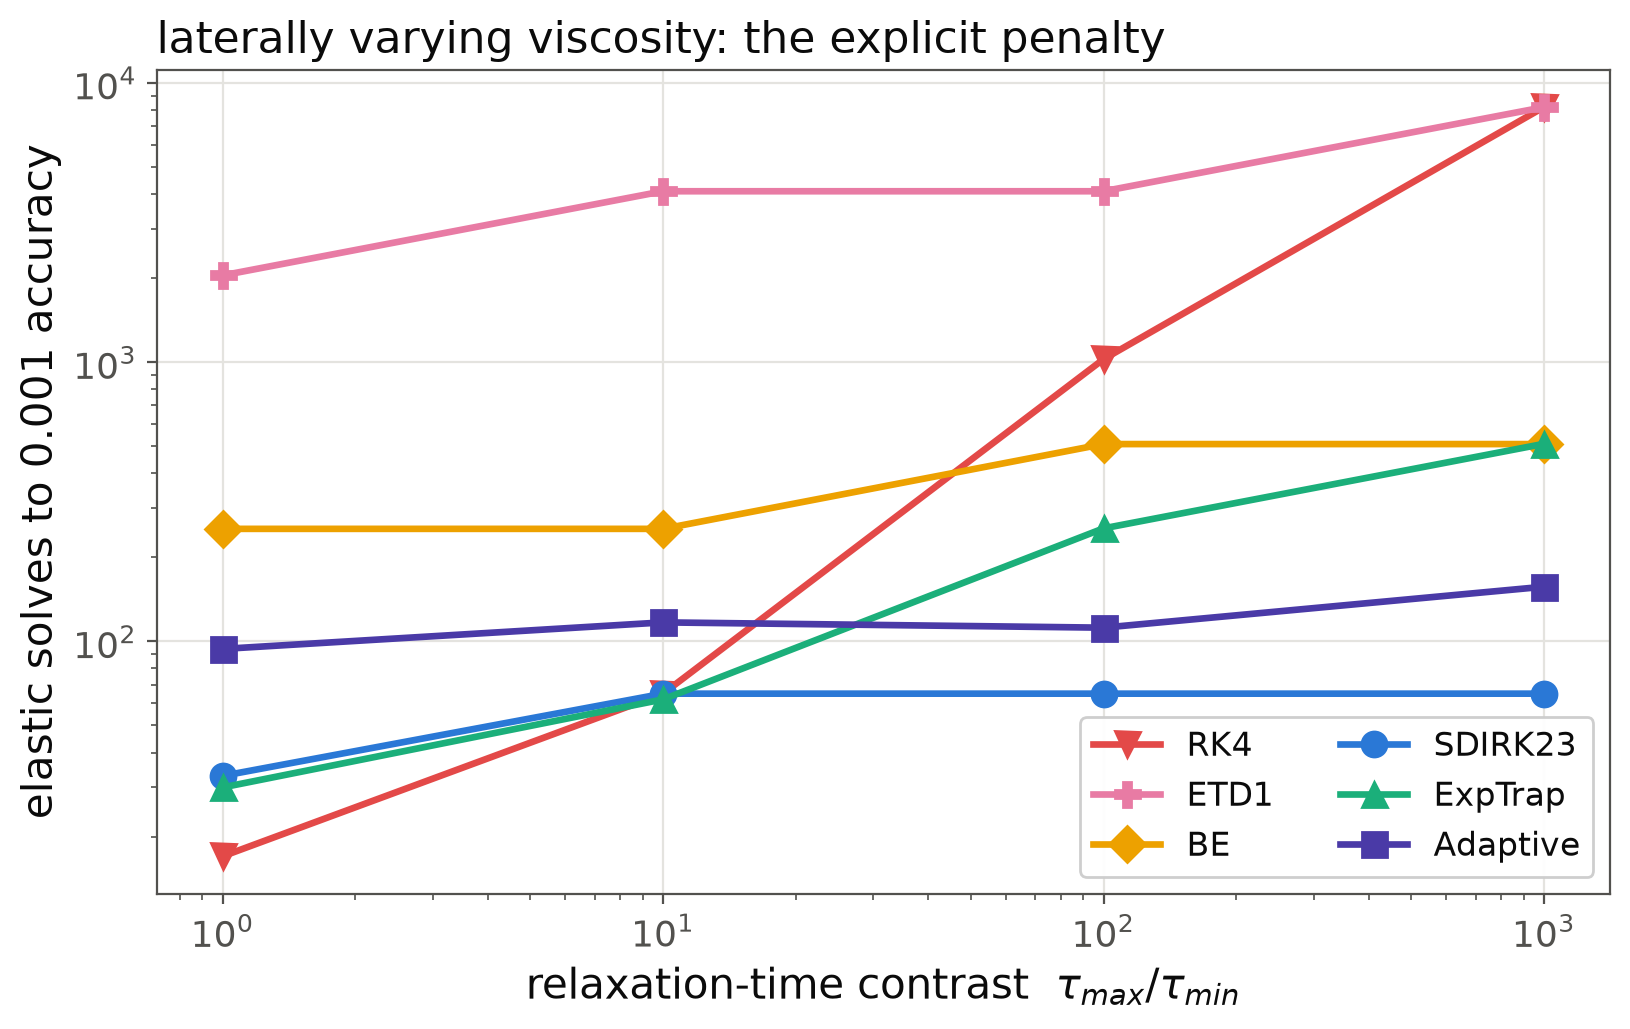
\includegraphics[width=0.48\textwidth]{ve_stiffness.png}\hfill
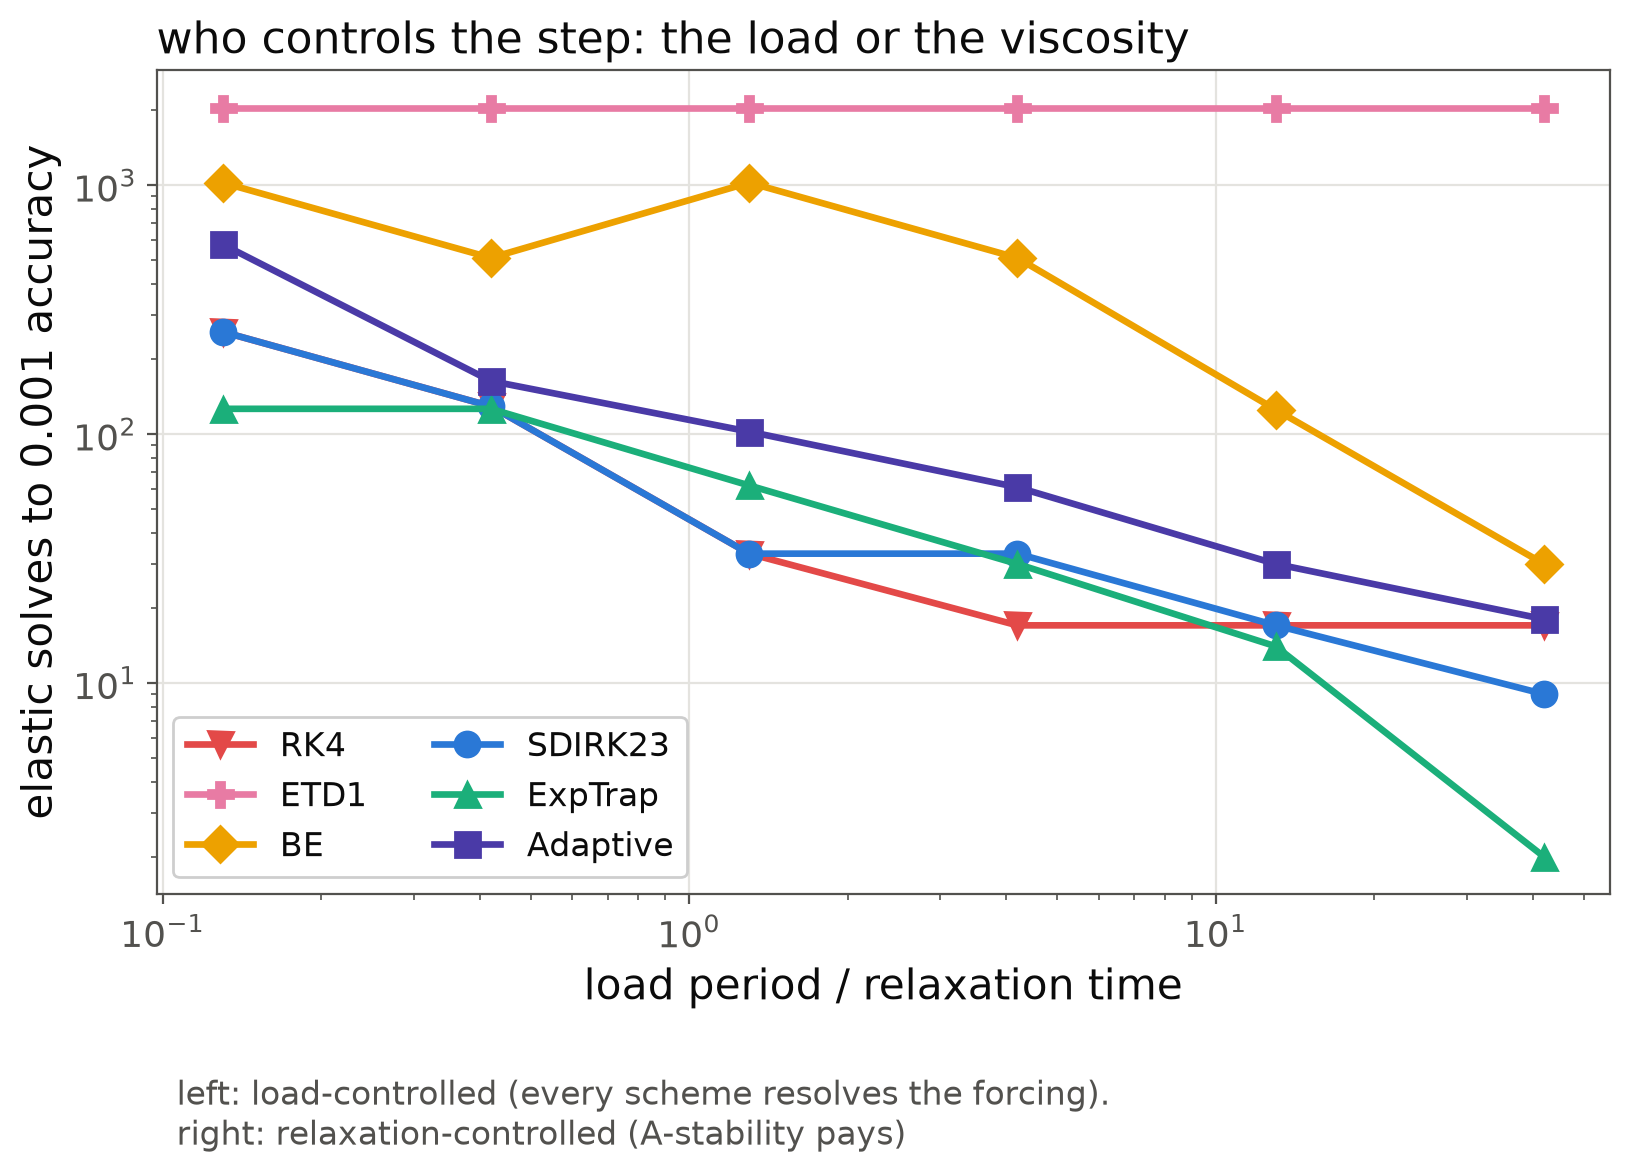
\includegraphics[width=0.5\textwidth]{ve_regimes.png}
\caption{Stepper survey: elastic solves to reach $10^{-3}$ against the
relaxation-time contrast (left) and against the load period (right).}
\label{fig:survey}
\end{figure}

\subsection{The Laplace-domain reference}
\label{sec:laplace}

\paragraph{What is computed.}
The reference gives the \emph{history} $f(t)$ of a Love number (any of
$h'_l,l'_l,k'_l$, and the tidal $h_l,l_l,k_l$) of a layered body whose
solid layers are Maxwell bodies (deviatoric relaxation, elastic in bulk,
relaxation time $\tau_j=\eta_j/\mu_j$), when the load is switched on at
$t=0$ and held: $f(0^+)$ is the elastic Love number, and $f(t)$ then
relaxes. pyslfp solves only \emph{elastic} problems, and only with real
moduli. The method below turns the viscoelastic history into a set of
elastic solves of modified models, then reassembles the history from them.

\paragraph{The correspondence principle.}
Write $F(s)=\int_0^\infty e^{-st}f(t)\,\mathrm{d}t$ for the Laplace
transform of the history. A Maxwell layer obeys
$\dot\sigma_d/(2\mu_j)+\sigma_d/(2\eta_j)=\dot\eps_d$ for the deviatoric
stress and strain. Its transform, for a body at rest at $t=0$, is
$\hat\sigma_d=2\mu_j(s)\hat\eps_d$ with
\begin{equation}
  \mu_j(s) = \mu_j\,\frac{s\tau_j}{1+s\tau_j},
  \label{eq:correspondence}
\end{equation}
which is Hooke's law with a modified shear modulus. Every other equation
(equilibrium, gravity, the boundary and interface conditions) is linear
with time-independent coefficients, so it transforms term by term,
unchanged. Bulk moduli, densities and fluid layers keep their values.
Hence, at each $s$, the transformed problem is an \emph{elastic} problem
for the body with the moduli \eqref{eq:correspondence}. Write $R(s)$ for
its Love number, the response to a unit load at that $s$. The load is the
Heaviside function, whose transform is $1/s$, so
\begin{equation}
  F(s) = \frac{R(s)}{s} .
  \label{eq:FR}
\end{equation}
For real $s>0$, $\mu_j(s)$ is real and lies in $(0,\mu_j)$. Each value
$R(s)$ is therefore an ordinary pyslfp elastic solve of a modified model.
The seismic velocities are rebuilt from the modified moduli, which
restricts the reference to models with uniform layers. The limits are
$R(\infty)=f(0^+)$, the elastic number, and, where it exists,
$R(0)=f(\infty)$, the fully relaxed one.

\paragraph{Why Gaver--Stehfest.}
It remains to invert the transform, recovering $f(t)$ from values of
$F$. The general inversion formula (the Bromwich integral) and its
accurate numerical versions (Talbot's contour, used in the box
sub-family, \S\ref{sec:box}) need $F$ at complex $s$, i.e.\ elastic
solves with complex moduli, which pyslfp does not provide. The
Gaver--Stehfest method needs $F$ on the positive real axis only, which is
why it is used.

\paragraph{How the inversion works.}
Fix $t$ and put $a=\ln 2/t$. Gaver's idea is to average $f$ against a
kernel that is concentrated at $u=t$ and whose average can be written in
terms of $F$. For an integer $m\ge1$ take
\begin{equation}
  f_m(t) = \int_0^\infty K_m(t,u)\,f(u)\,\mathrm{d}u,\qquad
  K_m(t,u) = a\,\frac{(2m)!}{m!\,(m-1)!}\,
             \bigl(1-e^{-au}\bigr)^m e^{-mau}.
\end{equation}
$K_m$ integrates to one in $u$, and it peaks where $e^{-au}=\tfrac12$,
i.e.\ at $u=\ln2/a=t$. This is the reason for the $\ln2$. Its width
shrinks like $1/\sqrt m$, so $f_m(t)\to f(t)$ as $m\to\infty$ for
continuous $f$. Expanding $(1-e^{-au})^m$ by the binomial theorem turns
each term into a Laplace transform:
\begin{equation}
  f_m(t) = a\,\frac{(2m)!}{m!\,(m-1)!}\sum_{j=0}^{m}(-1)^j\binom mj
           F\bigl((m+j)a\bigr).
\end{equation}
Each $f_m$ uses $F$ at the real points $s=(m+j)\ln2/t$ only. But
$f_m-f=O(1/m)$, which converges far too slowly. Stehfest accelerates the
sequence $f_1,\dots,f_{n/2}$ by a Richardson-type (Salzer) extrapolation
that eliminates the error terms in $1/m,1/m^2,\dots$. The combined
formula, with $n$ even the total number of transform values, is
\begin{equation}
  f(t) \approx a\sum_{k=1}^{n}V_k\,F(ka)
  \;\overset{\eqref{eq:FR}}{=}\;
  \sum_{k=1}^{n}\frac{V_k}{k}\,R\!\Bigl(\frac{k\ln 2}{t}\Bigr),
  \qquad a=\frac{\ln2}{t},
  \label{eq:stehfest}
\end{equation}
\begin{equation}
  V_k = (-1)^{k+n/2}\sum_{j=\lfloor (k+1)/2\rfloor}^{\min(k,n/2)}
   \frac{j^{n/2}(2j)!}{(n/2-j)!\,j!\,(j-1)!\,(k-j)!\,(2j-k)!}.
\end{equation}
The weights $V_k$ are fixed numbers once $n$ is chosen. The reference
uses $n=12$: twelve elastic solves per output time, at
$s=\ln2/t,\,2\ln2/t,\dots,12\ln2/t$, from which every Love number at
every degree is read.

\paragraph{Accuracy, and what limits it.}
Two errors compete.
\begin{itemize}[leftmargin=*]
\item \emph{Truncation.} The extrapolation is exact only in the limit.
  For smooth, non-oscillatory histories (sums of decaying exponentials,
  as here) $n=12$ gives four to six significant figures.
\item \emph{Amplification of errors in $R$.} The $V_k$ alternate in sign
  and grow rapidly with $n$, and the sum \eqref{eq:stehfest} cancels them
  almost entirely. A relative error $\delta$ in the values $R(s_k)$
  reaches $f$ multiplied by up to $\sum_k|V_k|/k$: $9.8\times10^3$
  ($n=8$), $3.4\times10^6$ ($n=12$), $1.3\times10^9$ ($n=16$). A larger
  $n$ therefore helps only if $R$ is correspondingly more accurate, and in
  double precision nothing is gained beyond $n\approx12$--$14$.
\end{itemize}
Both were measured on the box slabs against exact histories
(\S\ref{sec:box-stehfest}): with exact transform values, $n=12$ is
accurate to $10^{-6}$--$1.6\times10^{-4}$, and $n=16$ is no better. With
random relative noise of $10^{-10}$ in the transform, $n=12$ degrades a
small horizontal amplitude to $3\times10^{-4}$, and noise of $10^{-8}$
degrades it to $3\%$. The method also fails outright when $f$ grows
exponentially, since $F$ then has a pole at some real $s_p>0$; this is
the next paragraph.

\paragraph{The instability horizon.}
A compressible layer of uniform density has $N^2<0$. While its shear holds
it is stable, but once the shear relaxes, buoyancy is unopposed. The
transform then has poles on the positive real axis, the growth rates
$s_p$ of Rayleigh--Taylor-like modes. Stehfest's samples
$s_k=k\ln2/t\ge\ln 2/t$ are honest Laplace integrals of the (growing)
history only while $\ln2/t>s_p$. The script scans the real axis
(log grid, then a dense grid where the horizon is decided). A pole is a
bracket where $h'$ and $l'$ both change sign through large values. It
marks every time beyond $t_h=\ln2/\max s_p$ invalid. Measured ($\tau=1$):
\code{homogeneous} $s_p=0.0199$ ($t_h=35\tau$); \code{homogeneous\_lithosphere}
$0.0051$ ($136\tau$); \code{fluid\_core} $0.0085$ ($82\tau$). The default
output times, $0.011\cdot2^{5k/6}\tau$ for $k=0,\dots,12$ (to $11.3\tau$),
lie inside all three. The finite-element run carries the same growing
modes.

\paragraph{The relaxed limit is not $t\to\infty$.}
With no elastic layer the body relaxes to a fluid ball, and pyslfp
(rightly) refuses the relaxed solve. With an elastic layer, the
``relaxed'' solve (Maxwell layers at $\mu=0$) is pyslfp's \emph{static,
neutral} fluid. A non-neutral compressible Maxwell layer relaxes towards
its $\kappa$-response instead, and here towards no equilibrium at all.
The relaxed value is therefore a label, not a target: on
\code{homogeneous\_lithosphere}, $h'_2$ crosses it at about $7\tau$ and
keeps going (Figure~\ref{fig:series}).

\paragraph{Sanity checks.}
These are stored with the reference. The inversion at $t_0=10^{-6}\tau$
against the elastic numbers agrees to $10^{-6}$--$4\times10^{-6}$ (this is
the inversion's accuracy). Every $h',k',h,k$ history is monotone over the
valid times, with wiggles below ten times that accuracy forgiven. Where a
relaxed value exists, the script reports the fraction of the way to it,
as information only.

\subsection{The finite-element histories}

\paragraph{The driver.}
\code{viscoelastic\_love} loads a case exactly as \code{love\_benchmark}
does and gives each solid layer an \code{IsotropicMaxwellRheology}
(generalised Maxwell with $\mu_\infty=0$, one branch, $\kappa$ elastic) of
the case's own moduli, or keeps it elastic ($\tau=\infty$), through a
\code{CompositeRheology}. The problem is the Eulerian Dahlen class (or the
gauged one). At $t=0$ the loads $Y_{l0}$, $l_{\min}\le l\le l_{\max}$, are
switched on together, so one evolution serves every degree, and
\code{ViscoelasticOperator} advances the internal variables:
\begin{equation}
  \sigma = \kappa\,\mathrm{tr}\,\varepsilon\,I + 2\mu(d-m),\qquad
  \dot m = (d-m)/\tau,\quad d=\mathrm{dev}\,\varepsilon,\ m(0)=0 .
\end{equation}
The Love numbers are read at each output time by
\eqref{eq:loadlove}. Fixed-step schemes take, between consecutive output
times, the same number of equal steps: at least \code{-steps} (4) and
more if needed to keep $\Delta t\le0.25\tau_{\min}$. Output times are hit
exactly and are not tied to a step grid. SDIRK23 is the default.

\paragraph{The comparison metrics (\code{compare.py}).}
For each number $f$ and degree, over the valid output times together
with $t=0^+$:
\begin{align}
  \text{history} &= \frac{\max_t|f_{\text{FE}}(t)-f_{\text{ref}}(t)|}{\max_t|f_{\text{ref}}(t)|}, &
  \text{elastic} &= \frac{|f_{\text{FE}}(0^+)-f_{\text{ref}}(0)|}{|f_{\text{ref}}(0)|}, \\
  \text{relax} &= \frac{\max_t|\Delta f_{\text{FE}}(t)-\Delta f_{\text{ref}}(t)|}{\max_t|\Delta f_{\text{ref}}(t)|},
    & \Delta f(t) &= f(t)-f(0).
\end{align}
The history metric takes the worst time, not the final time alone, so
that a step that is right at one time and wrong at others cannot hide.
The \code{elastic} metric isolates the spatial error, and \code{relax}
isolates the error of the relaxation itself, which is what the stepping
answers for.

\paragraph{Results.}
Campaign (\code{fluid\_core}, $h=0.3$, order 2, $\tau_{\text{mantle}}=1$,
degrees 2--4, SDIRK23, 79 steps, 158 solves, 93\,s): the history errors
are $5\times10^{-3}$--$1.1\times10^{-2}$ in $h'$, $6\times10^{-3}$--$1.3\times10^{-2}$
in $k'$, and $1.5\times10^{-2}$, $6.3\times10^{-2}$, $0.46$ in $l'_{2,3,4}$.
The README records the stepping as not the limit: halving the step moves
$h',k'$ by about $2\times10^{-5}$. The errors are spatial and fall with
$h$ (\code{homogeneous} $h'_2$: $2.2\times10^{-2}\to1.0\times10^{-2}$ from
$h=0.3$ to $0.2$). $l'_4$ is the worst resolved. It is small, changes
sign, and its error grows late, where the buoyancy modes start to matter.
The new dense runs reproduce these numbers ($h'_2$ history
$1.09\times10^{-2}$ against $1.06\times10^{-2}$). The lithosphere model,
with its elastic lid, does better in $h'$ and $k'$ ($3\times10^{-3}$--$1.5\times10^{-2}$)
and in $l'_4$ (0.10).

\begin{figure}[H]
\centering
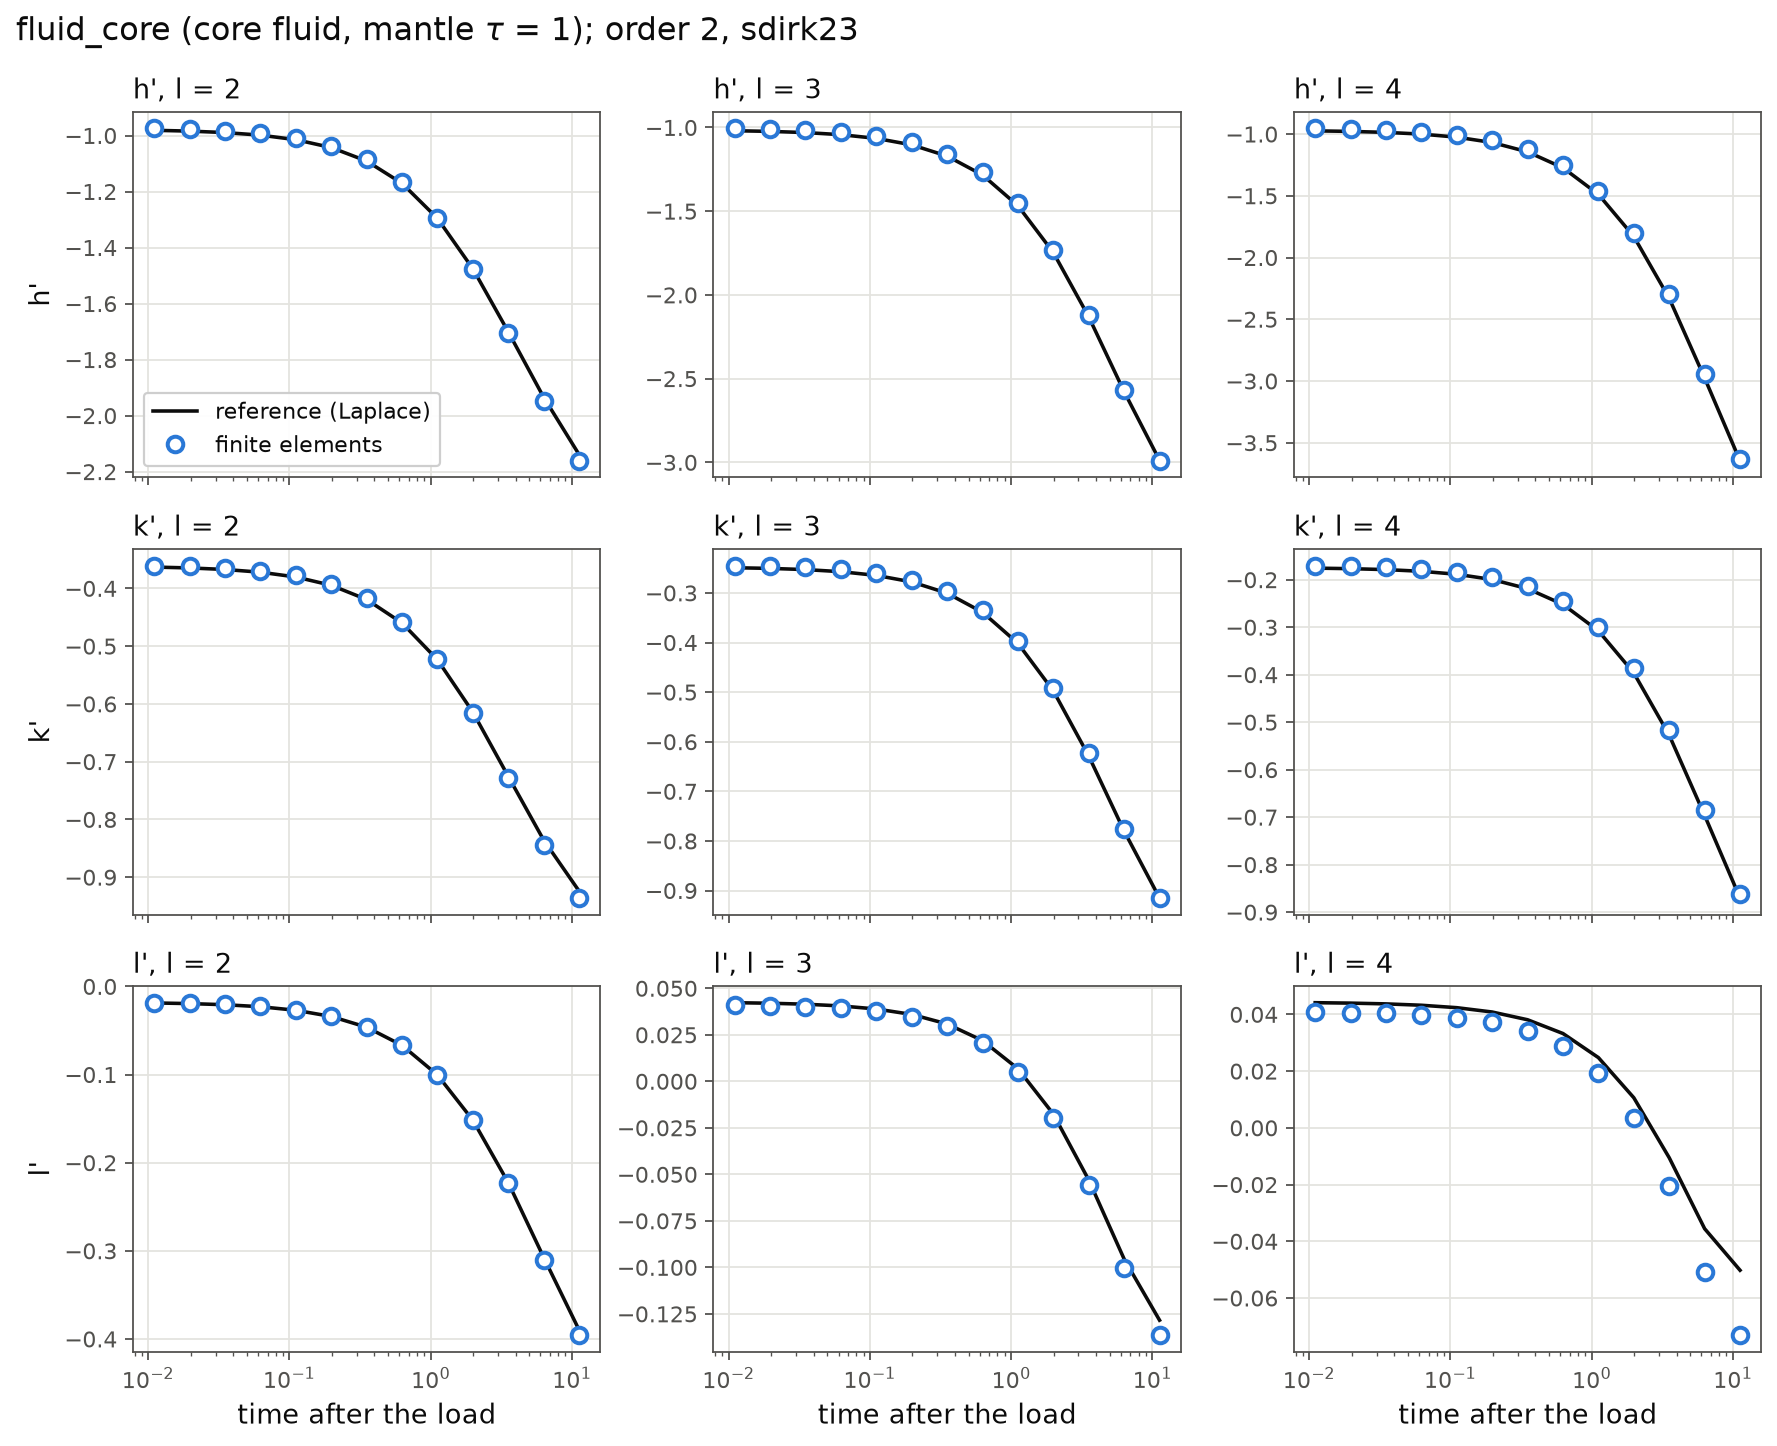
\includegraphics[width=0.75\textwidth]{ve_fc_history.png}
\caption{Campaign histories on a logarithmic time axis (\code{fluid\_core}):
reference (line) and FE (markers) at the 13 default times.}
\end{figure}

\begin{figure}[H]
\centering
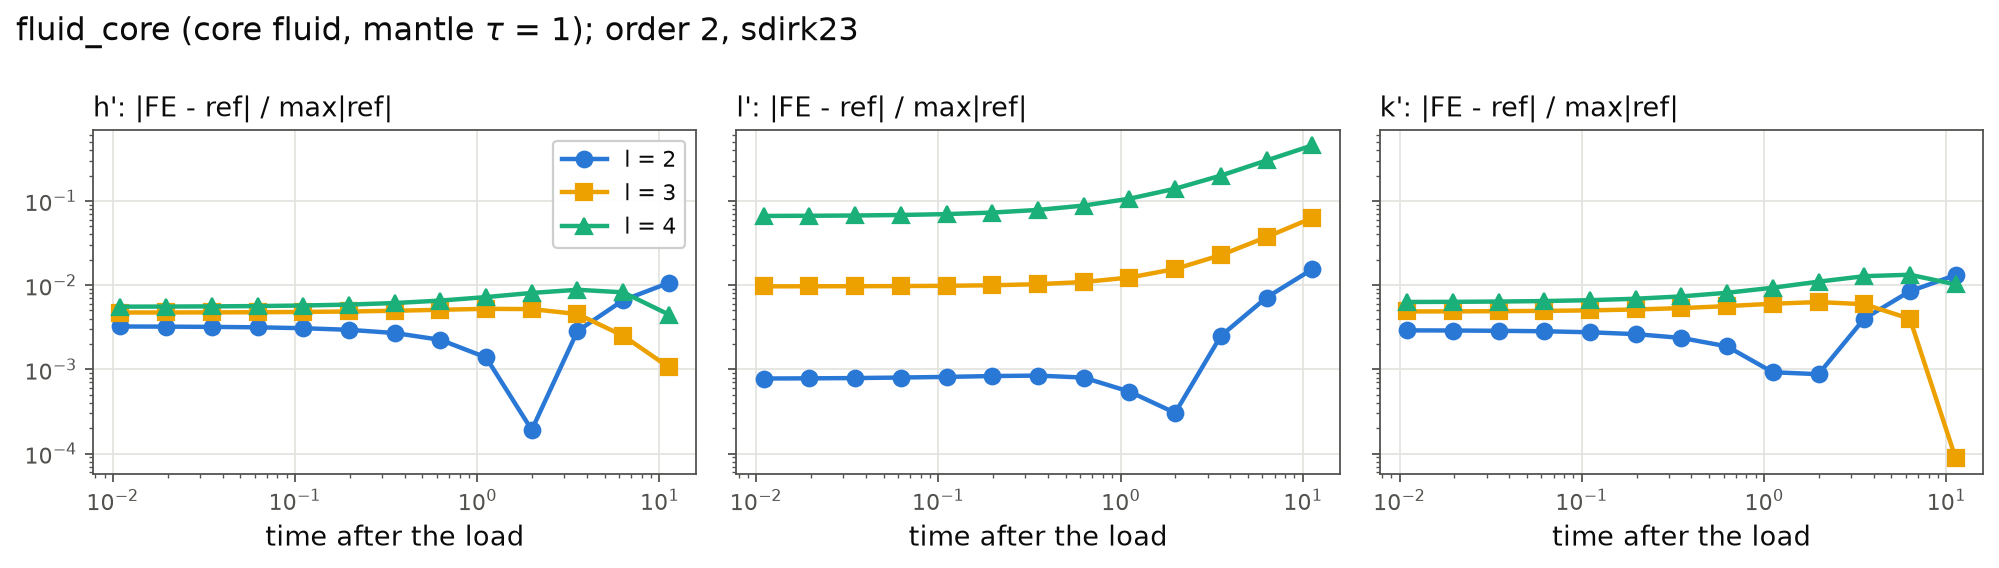
\includegraphics[width=0.85\textwidth]{ve_fc_error.png}
\caption{Pointwise error over the history, relative to the largest
reference value. The dip of $h'_2$ through zero near $t=2$ is why a
single-time check would mislead: it scores $2\times10^{-4}$ there against
a history error of $10^{-2}$.}
\end{figure}

\paragraph{Time series (new, Figure~\ref{fig:series}).}
For exposition, the histories are rerun at 48 equally spaced times
($0.25$--$12\tau$) on \code{fluid\_core} (Maxwell mantle) and on
\code{homogeneous\_lithosphere} (Maxwell interior under an elastic
$\approx670$\,km lid), with the reference at the same times
(pole scan off; both horizons are beyond $80\tau$). \code{compare.py}
draws them on a linear time axis when a run has 20 or more output times.
The figures show the shape of the relaxation that the logarithmic plots
hide: the immediate elastic jump, the roughly exponential approach on the
Maxwell scale, the faster relaxation of higher degrees, and on the
lithosphere model the overshoot of the static-fluid level, which is the
instability caveat of \S\ref{sec:laplace} made visible. Cost: 192 steps,
384 solves, about 400\,s each.

\begin{figure}[H]
\centering
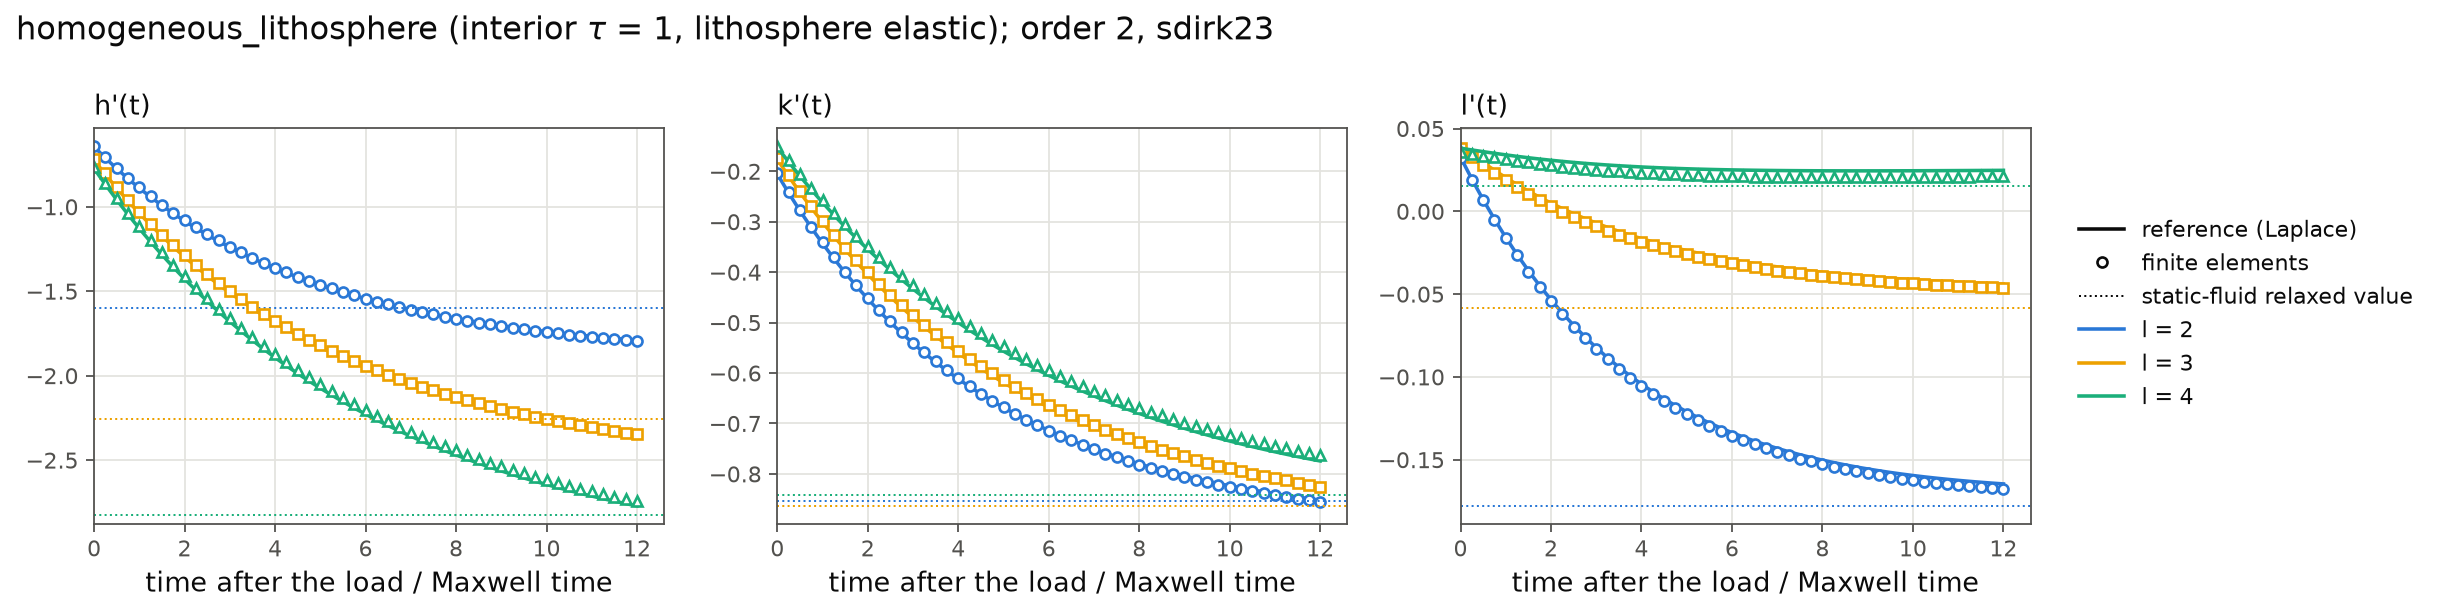
\includegraphics[width=\textwidth]{ve_hl_series.png}\\[1ex]
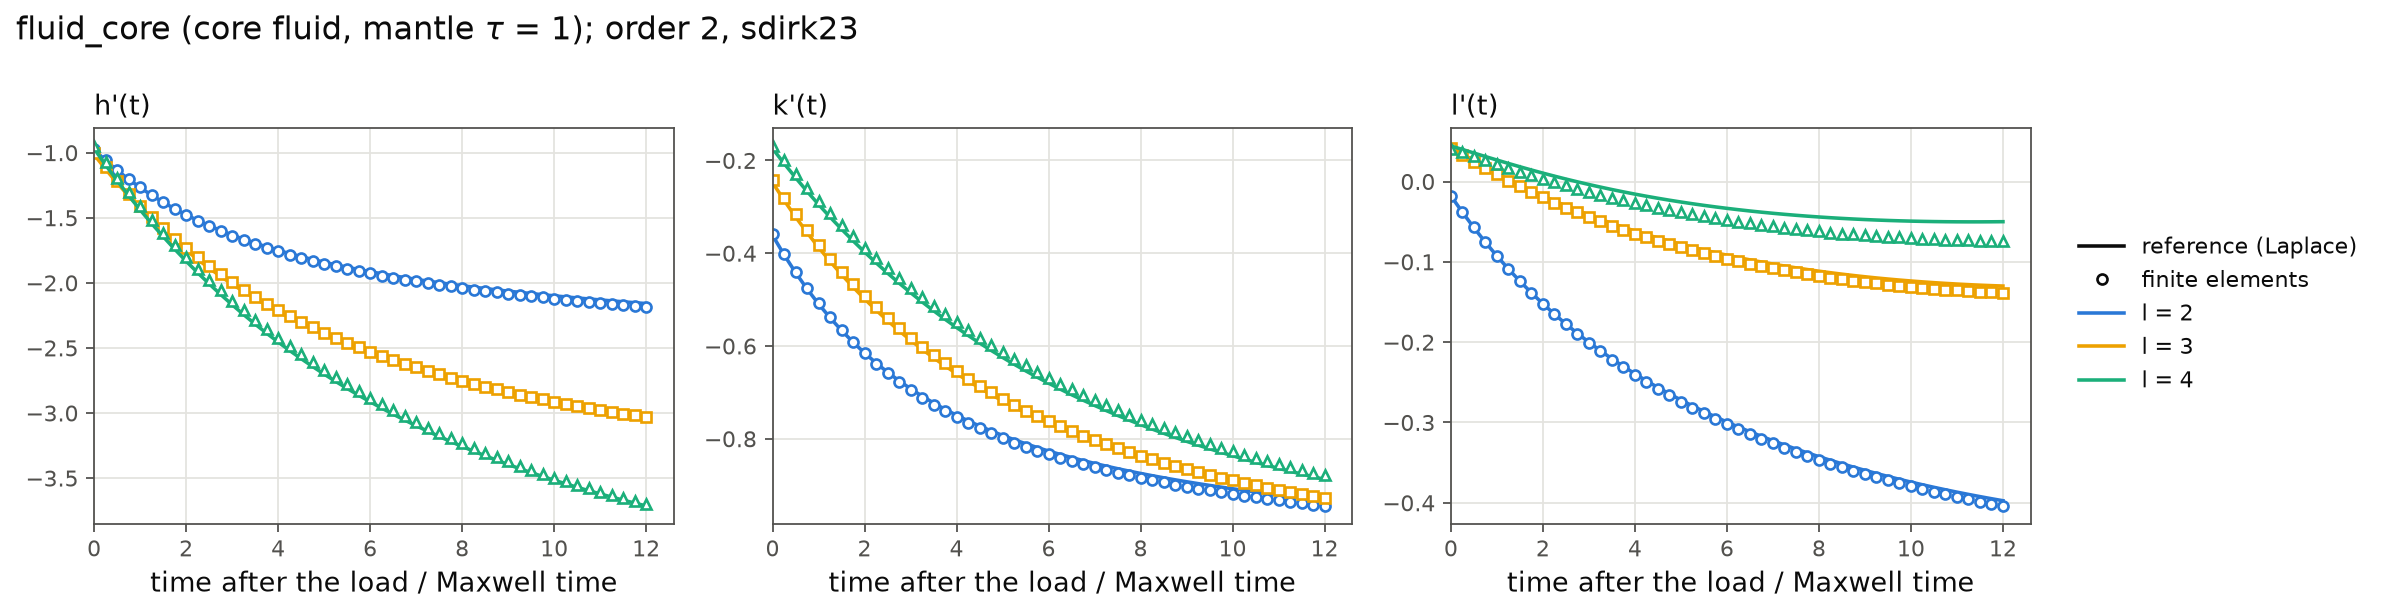
\includegraphics[width=\textwidth]{ve_fc_series.png}
\caption{Maxwell Love numbers in time, linear axis: reference (lines),
FE (markers, every other time), and the static-fluid relaxed value where
one exists (dotted). Top: \code{homogeneous\_lithosphere} (interior
$\tau=1$, elastic lithosphere); bottom: \code{fluid\_core} (mantle
$\tau=1$).}
\label{fig:series}
\end{figure}

\begin{figure}[H]
\centering
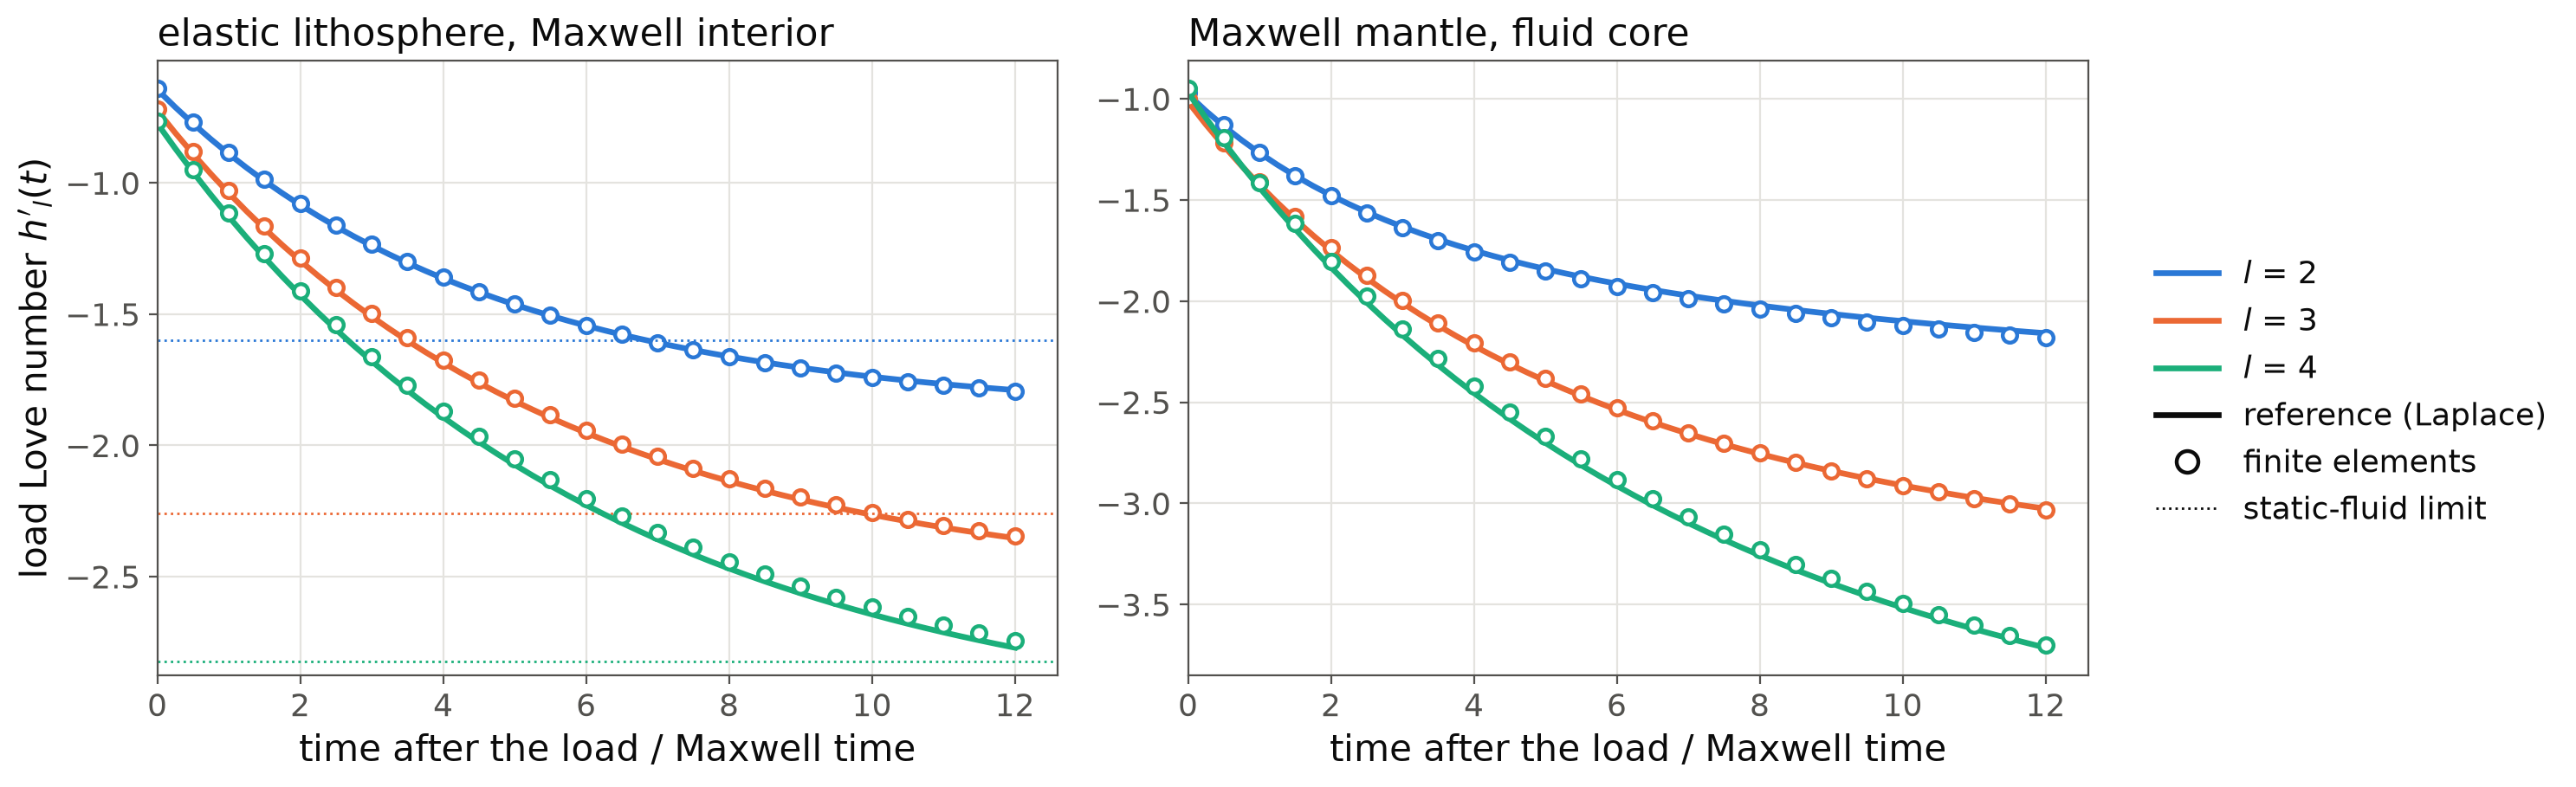
\includegraphics[width=\textwidth]{talk_viscoelastic.png}
\caption{Talk figure: $h'_l(t)$ for both models.}
\end{figure}

%=============================================================================
\section{Figure review}
\label{sec:figures}
%=============================================================================

\subsection{Changes made to the plotting scripts}

\begin{description}[leftmargin=1.5em,style=nextline]
\item[\code{love\_numbers/plot.py}]
  \begin{itemize}
  \item \emph{Bug}: field runs of different formulations shared one key
    (\code{h0.3\_o2}). The gauged field map overwrote the Dahlen one, the
    spectrum legend showed two identical labels, and
    \code{summary.md} attributed the gauged run's field errors (0.40) to
    the Dahlen row. Keys now carry the method. Maps are written per
    method, and titles name it.
  \item \emph{Bug}: the $h$-ladder grouped runs by order alone, so on a
    single-$h$ cross-method tree it fitted ``rates'' across formulations
    at one $h$ (vertical lines labelled $p=2.0$ etc.). Ladders are now
    per order and variant. A tree without a ladder draws no convergence
    figure and removes a stale one.
  \item \emph{Bug}: the convergence plot asked for the largest degree of
    any run, which only some rungs reached, so the second degree was
    silently dropped. It now uses the degrees every rung solved.
  \item \emph{Clarity}: colours were cycled from an 8-colour list, so
    with ten series two colours repeated, and colours changed between
    figures. Each formulation and CMB treatment now has one fixed colour,
    shared with \code{talk\_figures.py}. Order is shown by marker, the map
    by hollow markers, the Schur solver dotted, combined runs dashed, and
    the mesh size by lightness. \code{nomass}/\code{uniform} are drawn thin
    so that the full treatment shows through where they coincide.
  \item \emph{Clarity}: legends with up to ten entries sat on the data.
    They are now outside the panels. Element-size axes had no tick labels
    (a ladder spans less than a decade); they are now labelled at the
    sizes run, with near-coincident labels thinned. Fitted rates are
    printed beside the lines with a guide of slope $\text{order}+1$. The
    potential at degree one (zero by the choice of frame) is dropped
    from the field spectrum. Iterations are on a logarithmic axis, so the
    Dahlen and gauged costs are not flattened against the slipping ones.
  \end{itemize}
\item[\code{perturbation/plot.py}] Annotations overprinted each other
  ($h'_0$ and $l'_2$). Markers now encode the Love number and colours
  the degree. A third panel shows the relative discrepancy of each
  derivative, which is the actual result and was invisible on the
  identity plot for the small derivatives. The unmapped base run is
  labelled ``eps = 0 (unmapped)'' instead of ``eps = +0''.
\item[\code{viscoelastic/love/compare.py}] New \code{\_series.png}: linear-time
  histories with the elastic value at $t=0$ and the relaxed level. Layer
  labels read ``mantle $\tau=1$'' and ``lithosphere elastic'' instead of
  ``mantle 1''.
\item[\code{viscoelastic/stepping/survey.py}] The ``arrows'' caption is drawn only
  when an arrow is drawn, the stability limit quoted matches the code
  ($2.8\tau_{\min}$), and the regime caption wraps.
\item[\code{talk\_figures.py}] \code{aspherical.png} is rebuilt as error
  against amplitude from the genuine sweep; it had been labelling an
  $\eps=0.05$ run as $0.02$ and its halved-element run as $0.02$.
  \code{derivative.png} shows both methods from the 1 Oct runs (it had
  read the pre-fix 30 Sep slip\_broken runs), uses a legend instead of
  overprinting labels, and labels the axis as the 1-D reference, not
  ``perturbation theory''. New: \code{ladder.png}, \code{models.png},
  \code{viscoelastic.png}, \code{fieldmap.png}.
\end{description}

\subsection{Further suggestions (not done)}

\begin{itemize}[leftmargin=*]
\item \code{field3d.png} (ParaView) is a faceted half-ball with an
  unlabelled colour bar and much white space; \code{fieldmap.png}
  carries the same message more legibly. A better 3-D render would
  colour the whole sphere by $U$ with a diverging map and add the
  displacement arrows.
\item An accuracy--cost scatter (error against seconds per solve, one
  point per method and mesh) would summarise the methods comparison in
  one panel once a cross-method ladder exists.
\item \code{identity.png} hard-codes the slip value. A slip\_broken
  identity run in the campaign would let it read a log like the others.
\item A figure of the CMB report on a stratified core across $h$ (the
  deviation from full against the full treatment's own error) would show
  when the approximation becomes the bottleneck, which is the question
  the report asks.
\end{itemize}

%=============================================================================
\section{Points for review}
\label{sec:review}
%=============================================================================

These are things that look wrong, inconsistent or unexplained. They are
recorded, not fixed.

\begin{enumerate}[label=R\arabic*,leftmargin=*]
\item \label{r:gaugedfield} \textbf{Gauged field errors include the
  fluid.} \code{field\_benchmark} measures $\|\vu-\vu_{\text{ref}}\|$ over
  the whole displacement SubMesh, which for the gauged method includes
  the fluid core. There the reference displacement is written as zero,
  while the gauged displacement is a genuine (gauge-dependent) field.
  The 0.40 error of the gauged \code{fluid\_core} run is this artefact.
  The norm should be restricted to the solid attributes, or the fluid
  excluded from the comparison.
  \emph{Status 2 Oct:} fixed — \code{field\_benchmark} now takes the
  $u$ error over the solid elements alone and writes the fluid's norm
  separately (\code{u\_fluid\_norm}, a gauge diagnostic). Measured on
  \code{fluid\_core} h\,0.3/o2: gauged $u$ (solid) $1.9\times10^{-2}$
  (dahlen $1.3\times10^{-2}$), fluid gauge norm $0.046$ — the artefact
  explanation is confirmed.
\item \label{r:aspherical} \textbf{The stored amplitude comparison was
  not one.} \code{talk\_data/aspherical\_eps0.02\_o2.json} records
  $\eps=0.05$ and the stock mesh (built at the default
  $\eps=0.05$). It is the same problem as the $\eps=0.05$ run, which is
  why the two agreed to seven digits. The ``elements halved'' run is also
  at $\eps=0.05$, not $0.02$. The README's conclusion holds on the
  genuine sweep (\S\ref{sec:relabel}), but the README and the old talk
  figure state it on the wrong evidence. The driver's default
  \code{-eps 0.05} must match the mesh's $\eps$ by hand; nothing checks
  this (the mesh manifest could carry it).
  \emph{Status 2 Oct:} the mislabelled JSON is deleted;
  \code{aspherical\_body.py} now records $\eps$, $\beta$ and the buffer
  in the mesh manifest's \code{meta} block, and
  \code{aspherical\_reference} adopts them (a contradicting flag
  aborts). The driver also had, since commit \code{eac0b91}, a
  geometric seatbelt (the pulled-back surface must land on the unit
  sphere to $10^{-2}$) that would have refused a mismatched invocation
  — though not a misnamed output file, which is what actually happened.
\item \label{r:slipleak} \textbf{Lateral leakage in mapped slip\_broken.}
  Mapped slip\_broken runs have \code{spurious} 0.6 at $l=1$ and
  $6\times10^{-2}$ at $l\ge2$, against $3$--$8\times10^{-3}$ unmapped and
  unchanged for the welded referential. This fits the slipping-interface
  forms not being covariant (identity $1.2\times10^{-2}$), but the README
  describes the mapped runs as reproducing the unmapped ones without
  this caveat.
  \emph{Status 2 Oct:} the README now carries the caveat, and the code
  narrows the suspects: the $\varphi_e=\mathrm{id}$ mismatch-piece
  limitation documented in \code{referential\_problem.hpp} belongs to
  the \emph{single-valued} organisation, which refuses maps outright,
  while the broken-$\zeta$ organisation that slip\_broken uses is
  intended fully mapped — so some term of it is non-covariant in a way
  its own documentation does not know.
  \emph{Further, same day:} the identity driver now probes the sixteen
  broken-$\zeta$ blocks and the stored constraint kernels. Every
  $\zeta$--$\zeta$ block agrees to machine precision; every
  $u$-involving block differs at $1$--$2.5\times10^{-4}$; the kernels
  are exonerated ($B_n$ at $2\times10^{-16}$ — the Nanson
  $\nu=\mathrm{adj}(F)^T n$ is invariant under face-fixing shears of
  $F$ — and $P_b$, $K_{vz}$ at $10^{-7}$), and the base rows are
  welded-certified, so by elimination the non-covariant content sits in
  $B_\Sigma$/$G_\Sigma$ themselves: the $P_T F^{-1}$ slot and the
  gravity $\mathbf{A}$-vector are not invariant under those shears,
  which the interpolated $F$ carries on the interface (MFEM evaluates
  $F$ from the adjacent volume element). The identity residual
  \emph{anti-converges} ($u$ $1.2\times10^{-2}$ at $h=0.3$,
  $4.5\times10^{-2}$ at $h=0.2$), a genuine defect rather than
  interpolation noise. Two further probes of the exact-$F$ benchmark
  leakage: (i) $G_\Sigma$ cannot be scaled out differentially — at
  \code{-gs-scale 0.5} even the \emph{unmapped} degree-1 spurious blows
  up to $0.46$ (and the mapped solve diverges), so $G_\Sigma$ sits
  inside a razor-sharp degree-1 cancellation and the mapped leakage is
  plausibly a small relative perturbation of it, hugely amplified;
  (ii) the slip rigid null-pair residuals (now printed by
  \code{love\_benchmark -diag}) survive the map essentially unchanged
  (translations $2.4$ vs $2.6\times10^{-3}$, rotations doubled at
  $\sim10^{-3}$), so the null-pair structure itself is not broken.
  Settling the exact-$F$ mechanism needs either a $B_\Sigma$
  counterpart of the scale hook, a difference-field map of the
  mapped-vs-unmapped solutions, or a theory pass on the mapped
  $B_\Sigma$/$G_\Sigma$ derivation (doc/slip\_interface.tex) — the
  degree-1 cancellation identifies exactly which combination must be
  preserved by the mapped assembly.
\item \label{r:pertslip} \textbf{slip\_broken degree-2 derivatives.} The
  README says the slip\_broken derivatives agree ``at the few-percent
  level'' for degrees 3--4. The 1 Oct data give $h'_2$ 25\,\%, $k'_2$
  39\,\%, $k'_3$ 11\,\%, against 6.5\,\%, 1.8\,\% and 0.9\,\% for
  referential on the same mesh. The two methods share the shift map and
  the reference, so the difference sits in the slipping forms under a
  moving interface. Possibly the same non-covariance as
  \ref{r:slipleak}. \emph{Status 2 Oct:} open; see \ref{r:slipleak}'s
  status — the same scheduled diagnostic covers both.
\item \label{r:cmbclaim} \textbf{``Loading-safe, $\le0.1\,\%$''.} The top-level
  README states the CMB approximations are within 0.1\,\% for loading at
  $l\ge2$. That holds for $h'$ (the table in \code{cmb\_conditions.md} is
  $h'$ only). $l'_2$ and $k'_2$ deviate by about 0.3\,\%, and the talk
  figure shows $k'_2$ at 0.29\,\%. Still below the mesh error, but the
  sentence should say which number.
  \emph{Status 2 Oct:} fixed — the README names $h'$ and the
  $\sim0.3\,\%$ of $l'_2$, $k'_2$.
\item \label{r:ladder} \textbf{The \code{fluid\_core} ladder is not
  asymptotic.} Order 3 is flat from $h=0.3$ to $0.15$ and then drops by
  10--100$\times$ at $0.12$ alone, and the geometry-order-3 ladder is
  less accurate than geometry order 2 and does not drop. The angular cap
  holds the CMB elements at $0.165$ for $h\ge0.165$, which explains some
  of the flatness (half the ladder does not refine the CMB) but not the
  drop. Candidates: a cancellation at $0.12$, a floor from the DtN
  degree (16) or the reference, or the geometry. The fitted rates of
  this ladder should not be quoted as convergence orders.
  \emph{Status 2 Oct:} the cap arithmetic is confirmed in planetmodel
  ($\min(h, 0.3r)$ with $r_{\text{cmb}}=0.549\to0.165$); an uncapped
  ladder (\code{--angular 1.0}, every rung refining the CMB) now lives
  in \code{runs\_campaign/ladder}. On it the order-3 flat-then-cliff is
  gone: the degree-2 scaled error falls monotonically-ish
  ($7.7\times10^{-3}\to2.5\times10^{-5}$ over $h=0.3\to0.12$, one
  non-monotone rung at $0.15$), and the field errors fall throughout —
  but the implied degree-2 rate ($\sim6$) is superconvergent, so the
  Love-number columns still carry cancellation and fitted rates should
  still not be quoted; the field-error rates are the quotable ones.
\item \label{r:gaugedprofile} \textbf{Gauged $\phi_1$ inside the core.}
  In \code{profiles.png} the gauged method's degree-1 potential leaves the
  reference inside the fluid core ($r\lesssim0.5$) while matching at the
  interfaces. It may be the degree-one frame correction (applied with the
  background gravity of the profile layer) or the gauge, but it is
  unexplained.
  \emph{Status 2 Oct:} measured and sharpened — it is the formulation,
  not the plot. The degree-1 $\phi$ profile's relative RMS deviation
  from the reference is, for the gauged method, $0.119$ in the core and
  $0.053$ in the mantle at $h=0.3$, and $0.120$/$0.056$ at $h=0.2$ —
  flat in $h$ — while dahlen's falls with refinement
  ($0.013\to0.010$ core). It is also flat in the gauge
  $\eps\in[10^{-2},10^{-1}]$ and in the refinement count, and $\phi$ is
  gauge-invariant under exact relabellings, so this is a systematic
  $\sim12\,\%$ defect of the gauged formulation's degree-1 interior
  response (its surface values stay at the 1\,\% level). The gauged
  formulation's degree-1 terms need review before the method is used
  for interior fields.
\item \label{r:identityheader} \textbf{Stale header in
  \code{relabelled\_identity.cpp}.} The header comment still says that the
  gauge penalty is ``the one non-covariant assembly piece'' and that the
  identity is informational where gauge machinery runs. The code (strict
  for every welded case) and the README (covariant penalty, $1.6\times10^{-7}$)
  say otherwise. The same run prints a gauge semi-convergence warning
  (contraction 0.95 at $\eps=10^{-2}$), which does not affect the identity
  but says the gauge refinement is not contracting on that mesh.
  \emph{Status 2 Oct:} the header is rewritten to match the code (strict
  on every welded case; the slip leg informational with the
  non-covariant term unlocalised). The semi-convergence itself remains
  open — the gauged field run on \code{fluid\_core} h\,0.3 prints
  contraction $1.013$, and the gauged solid field error is insensitive
  to $\eps\in[10^{-2},1]$ and to the refinement count.
\item \label{r:worst} \textbf{``Worst error'' columns are $l'$ columns.}
  The summaries' worst-of-six error at degree 2 is nearly always $l'_2$,
  a small number (e.g.\ $-0.0175$ on \code{fluid\_core}), so the column
  reads 17\,\% for methods whose $h'$, $k'$ are at 1\,\%. A relative error
  against $\max(|x_{\text{ref}}|,\text{scale})$, or per-number columns,
  would be more informative.
  \emph{Status 2 Oct:} fixed — the summary columns now use a scaled
  error (each quantity against its own largest reference value over the
  degrees) and are headed ``worst scaled error''; \code{fluid\_core}
  degree 2 reads $1$--$2\times10^{-2}$ across the methods.
\item \label{r:derivlabel} \textbf{``Perturbation theory'' label.} The
  1-D side of the derivative check is a central difference of pyslfp
  solves, not a perturbation-theory kernel. The old talk figure's axis
  said ``perturbation theory (1-D reference)''. Relabelled; worth
  keeping distinct until the adjoint kernels exist.
\item \textbf{Survey stability statement.} \code{survey.py}'s caption
  said $\Delta t\lesssim\tau_{\min}$ while the code, the example and the
  README say $2.8\tau_{\min}$ (RK4). Corrected in the caption.
\item \textbf{Mixed-vintage data in the summaries.} \code{love\_numbers/runs}
  (28 Sep) predates later solver changes (gauge penalty, AL tolerances),
  and \code{runs\_methods} (30 Sep) contains slip\_broken shift runs
  made before the outward-shift fix. The talk figures read from both.
  Before any external use the methods and model sweeps should be rerun
  on the current code; the campaign script can do this unattended.
  \emph{Status 2 Oct:} done — \code{runs\_campaign}'s stale results
  (its slip rows, 30 Sep, predated the 1 Oct slip fix) were moved to
  \code{runs\_campaign\_stale\_20261002} and the local campaign, the
  model sweep (h\,0.2, orders 2 and 3, eight models), the prem\_4 CMB
  variants and the uncapped ladder were rerun on the current code (all
  stages ok); \code{talk\_figures.py}'s defaults now read
  \code{runs\_campaign} throughout and all nine talk figures are
  regenerated, retiring \code{love\_numbers/runs} and
  \code{runs\_methods}. On the current code the mapped slip\_broken
  leakage persists at about half strength (\code{spurious} 0.36 at
  $l=1$, $6$--$9\times10^{-2}$ at $l\ge2$).
\end{enumerate}

\end{document}
